\documentclass{article}

% Formatting
\usepackage[utf8]{inputenc}
\usepackage[margin=1in]{geometry}
\usepackage[titletoc,title]{appendix}
\usepackage[spanish]{babel}
\usepackage{amsmath,amsfonts,amssymb,mathtools}
\usepackage{graphicx,float}
\usepackage[ruled,vlined]{algorithm2e}
\usepackage{algorithmic}
\usepackage{minted}
\usemintedstyle{borland}
\usepackage{subcaption}
\usepackage{multicol}
\usepackage{listings}
\usepackage{xcolor}
\usepackage{biblatex}
\addbibresource{ref.bib}
\usepackage{minted}



% Title content
\title{Práctica 8 modelo de urnas}
\author{Denisse Leyva}
\date{Abril 21, 2021}

\begin{document}

\maketitle


\section{Introducción}
La octava práctica es sobre fenómenos de coalescencia y fragmentación, donde partículas se unen para formar cúmulos y estos cúmulos se pueden volver a descomponer en fragmentos menores. Esto es relevante en muchos campos de química, como por ejemplo en el filtrado de aguas residuales, donde solamente los cúmulos de suficiente tamaño serán capturadas por el filtro y hay que buscar formas para facilitar que crezcan los cúmulos de residuos para lograr su filtrado adecuado.

Vamos a suponer que tenemos una cantidad total de $n$ partículas y que al inicio el tamaño de los $k$ cúmulos existentes sigue la distribución normal. Para lograr esto, vamos a crear $k$ valores de la distribución normal estándar (media cero, desviación estándar uno) y luego normalizarlos para convertirlos en enteros positivos que sumen a $n$ \cite{Satu_Elisa_Schaeffer}.

\section{Objetivo}
Supongamos que cúmulos con $c$ o más partículas (haciendo referencia al tamaño crítico c) son suficientemente grandes para filtrar. Gráfica $k=1000, n \in {16k,32k, 64k, 128k}$ en cada iteración $t$ el porcentaje de las partículas que se logra filtrar \cite{Satu_Elisa_Schaeffer}.

\section{Código}
\renewcommand{\listingscaption}{Código}
\begin{listing}[H]
  \begin{minted}[linenos,mathescape,texcl]{clojure}
  def filtro(cumulos, c, n):
    cum = []
    for valor in cumulos:
        if valor >= c:
            cum.append(valor)
    porcentaje = (sum(cum)*100)/n
    return porcentaje
      \end{minted}
  \label{lst:fibo}
  \caption{Obtener el porcentaje del valor filtrado.}
\end{listing}

\section{Resultados}
Para obtener las gráficas se realizaron 50 réplicas con una duración de 50 pasos, por lo tanto nos muestran el porcentaje filtrado mayor o igual al valor crítico. El código completo se encuentra en GitHub \cite{Denisse_Leyva}. El código base se obtuvo de Schaeffer \cite{Elisa_Schaeffer}.

\begin{figure}[H]
\centering
\begin{subfigure}[b]{0.40\linewidth}
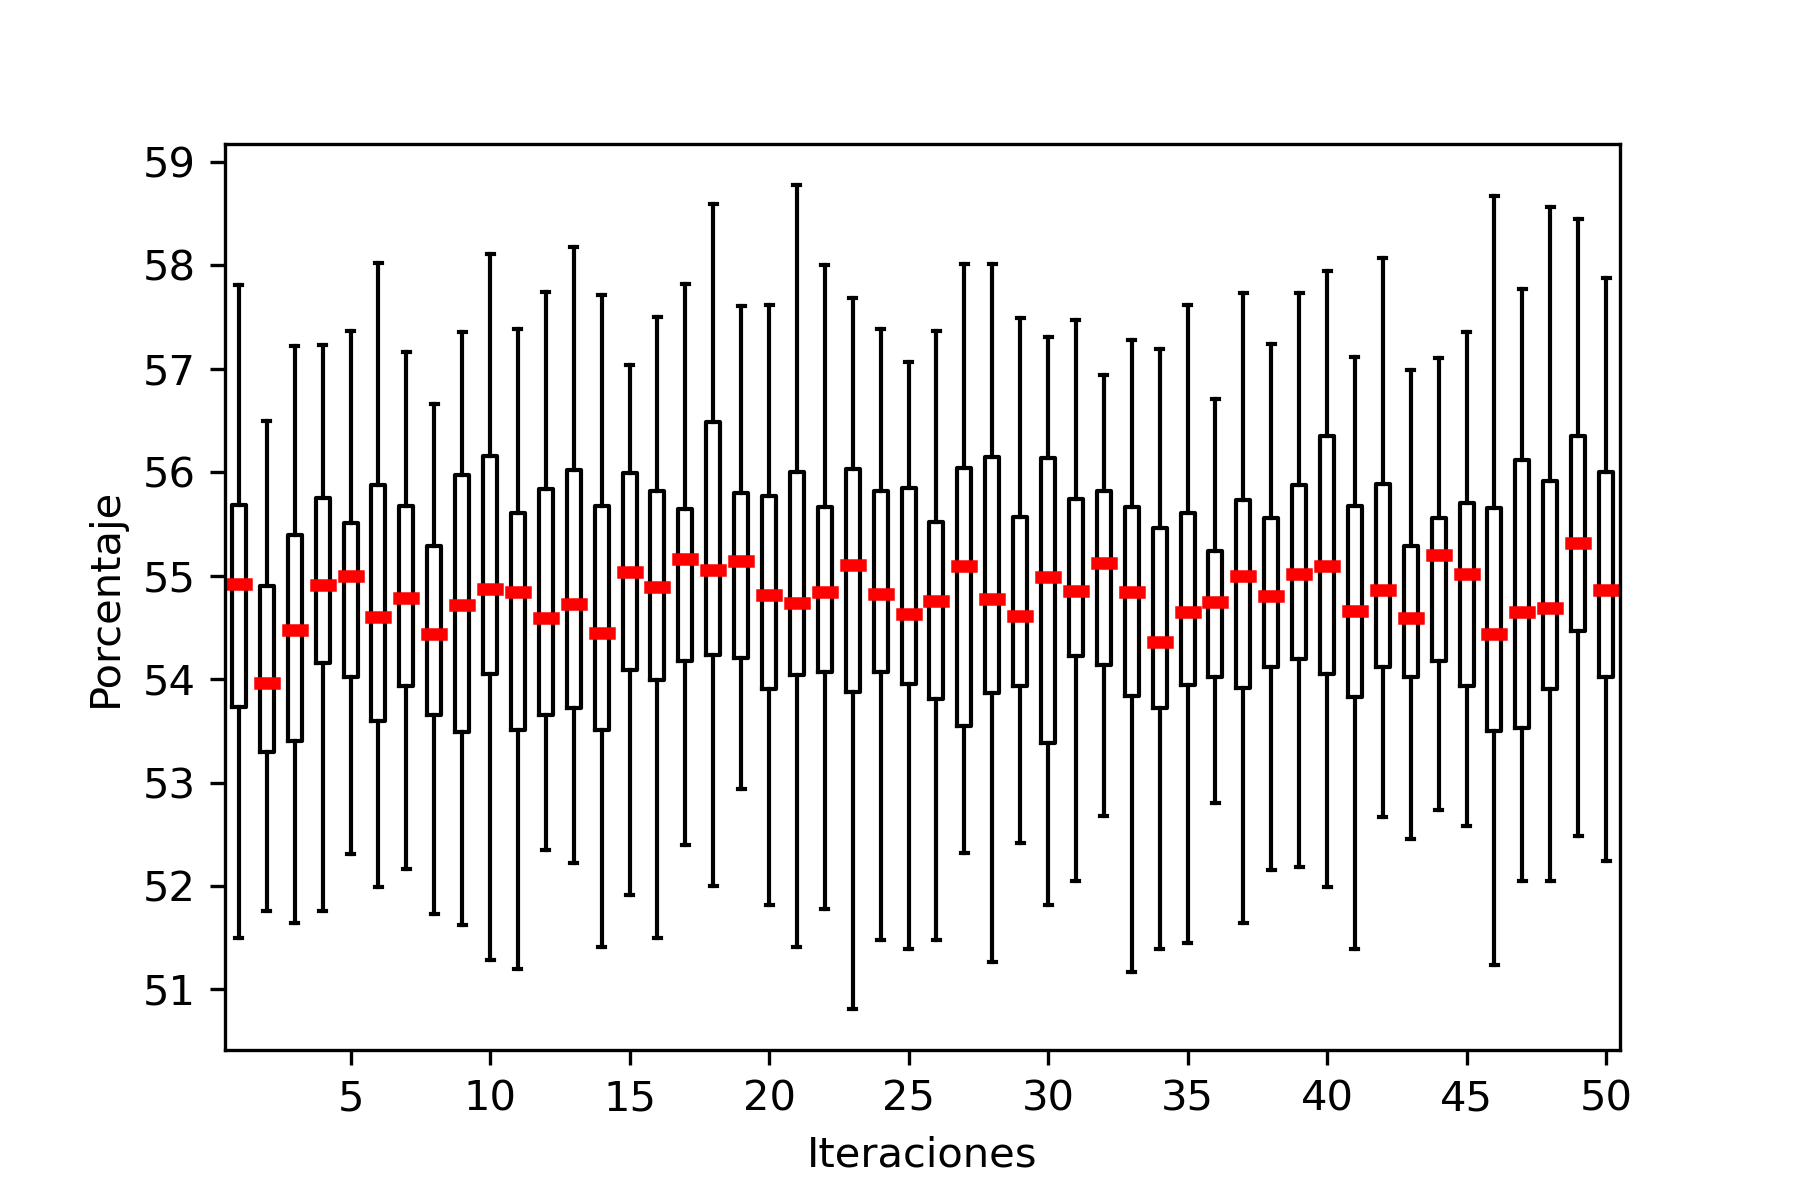
\includegraphics[width=\linewidth]{p8_n16000.png}
\caption{16000 partículas.}
\end{subfigure}
\begin{subfigure}[b]{0.40\linewidth}
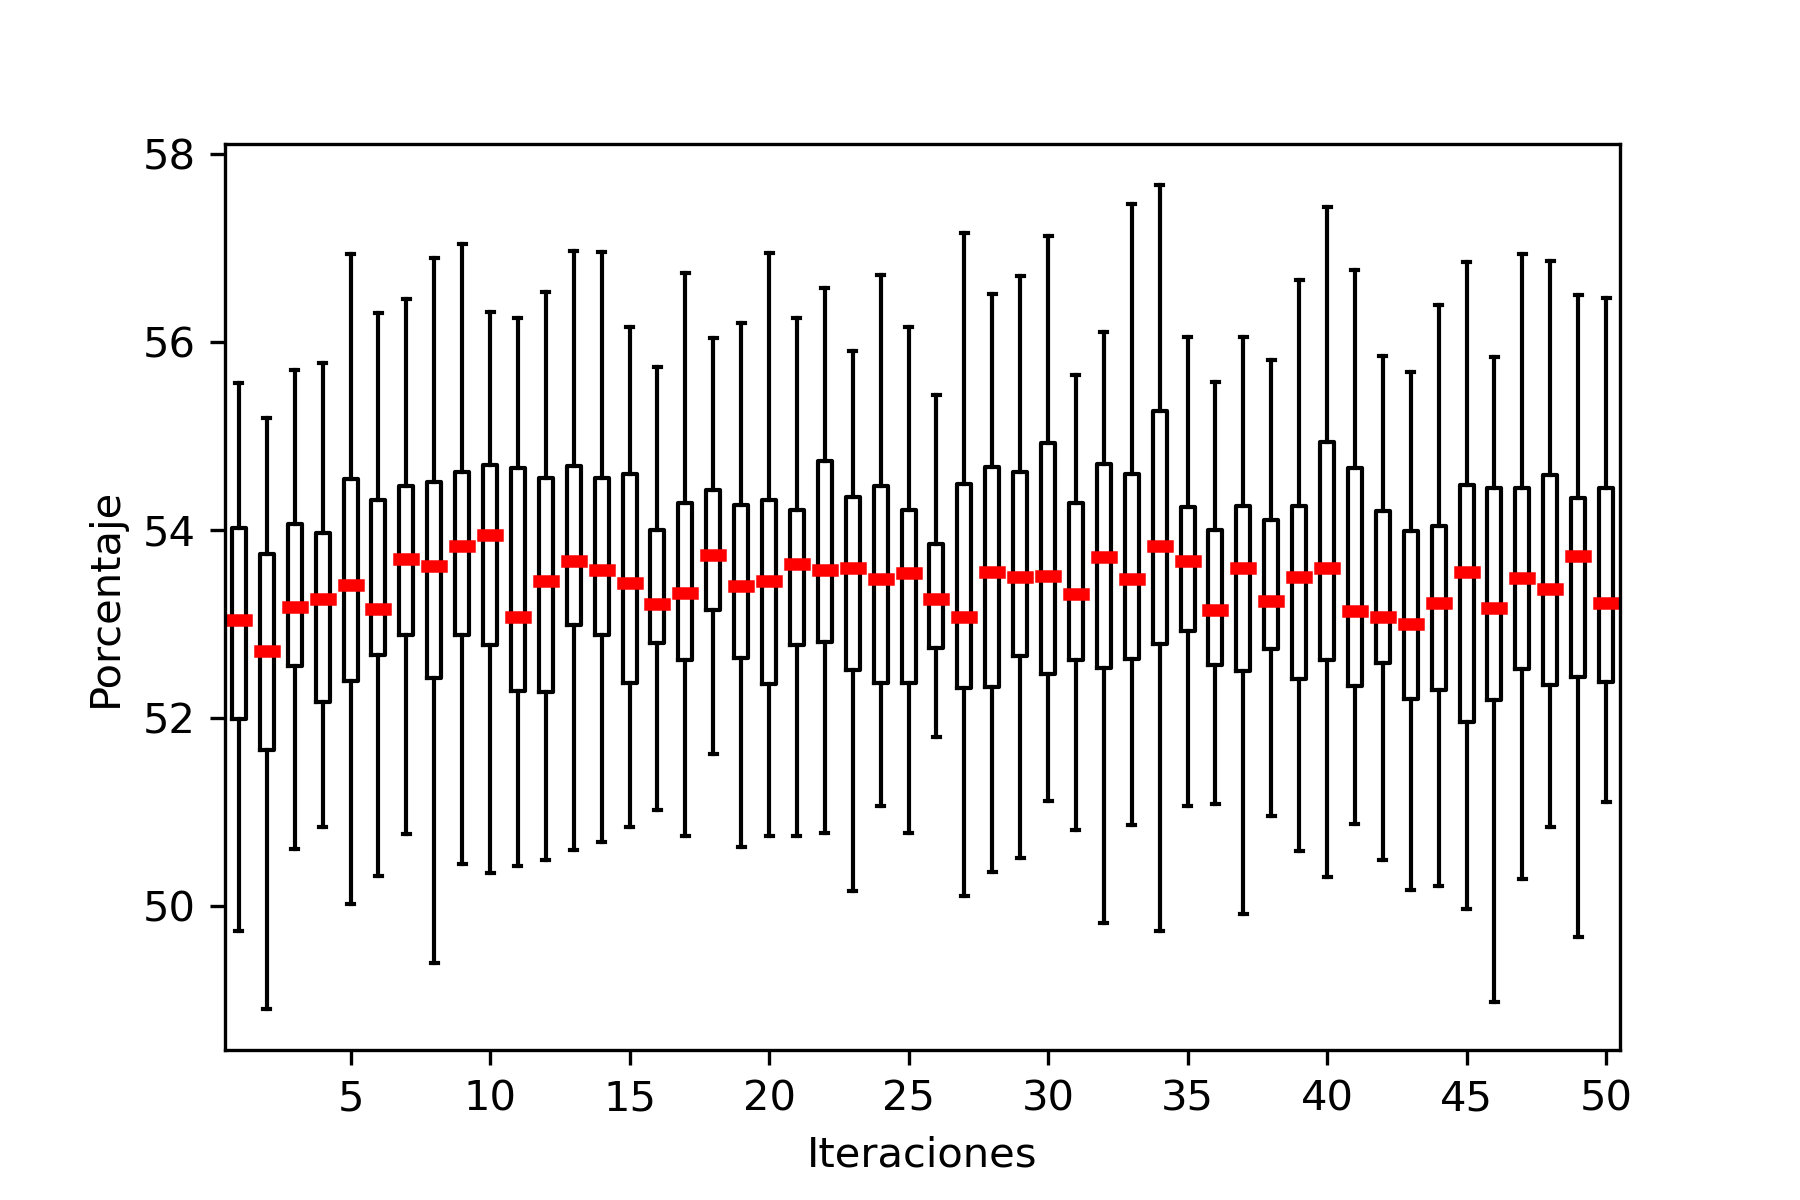
\includegraphics[width=\linewidth]{p8_n32000.png}
\caption{32000 partículas.}
\end{subfigure}
\caption{Porcentaje filtrado por iteración.}
\label{fig:westminster}
\end{figure}

\begin{figure}[H]
\centering
\begin{subfigure}[b]{0.40\linewidth}
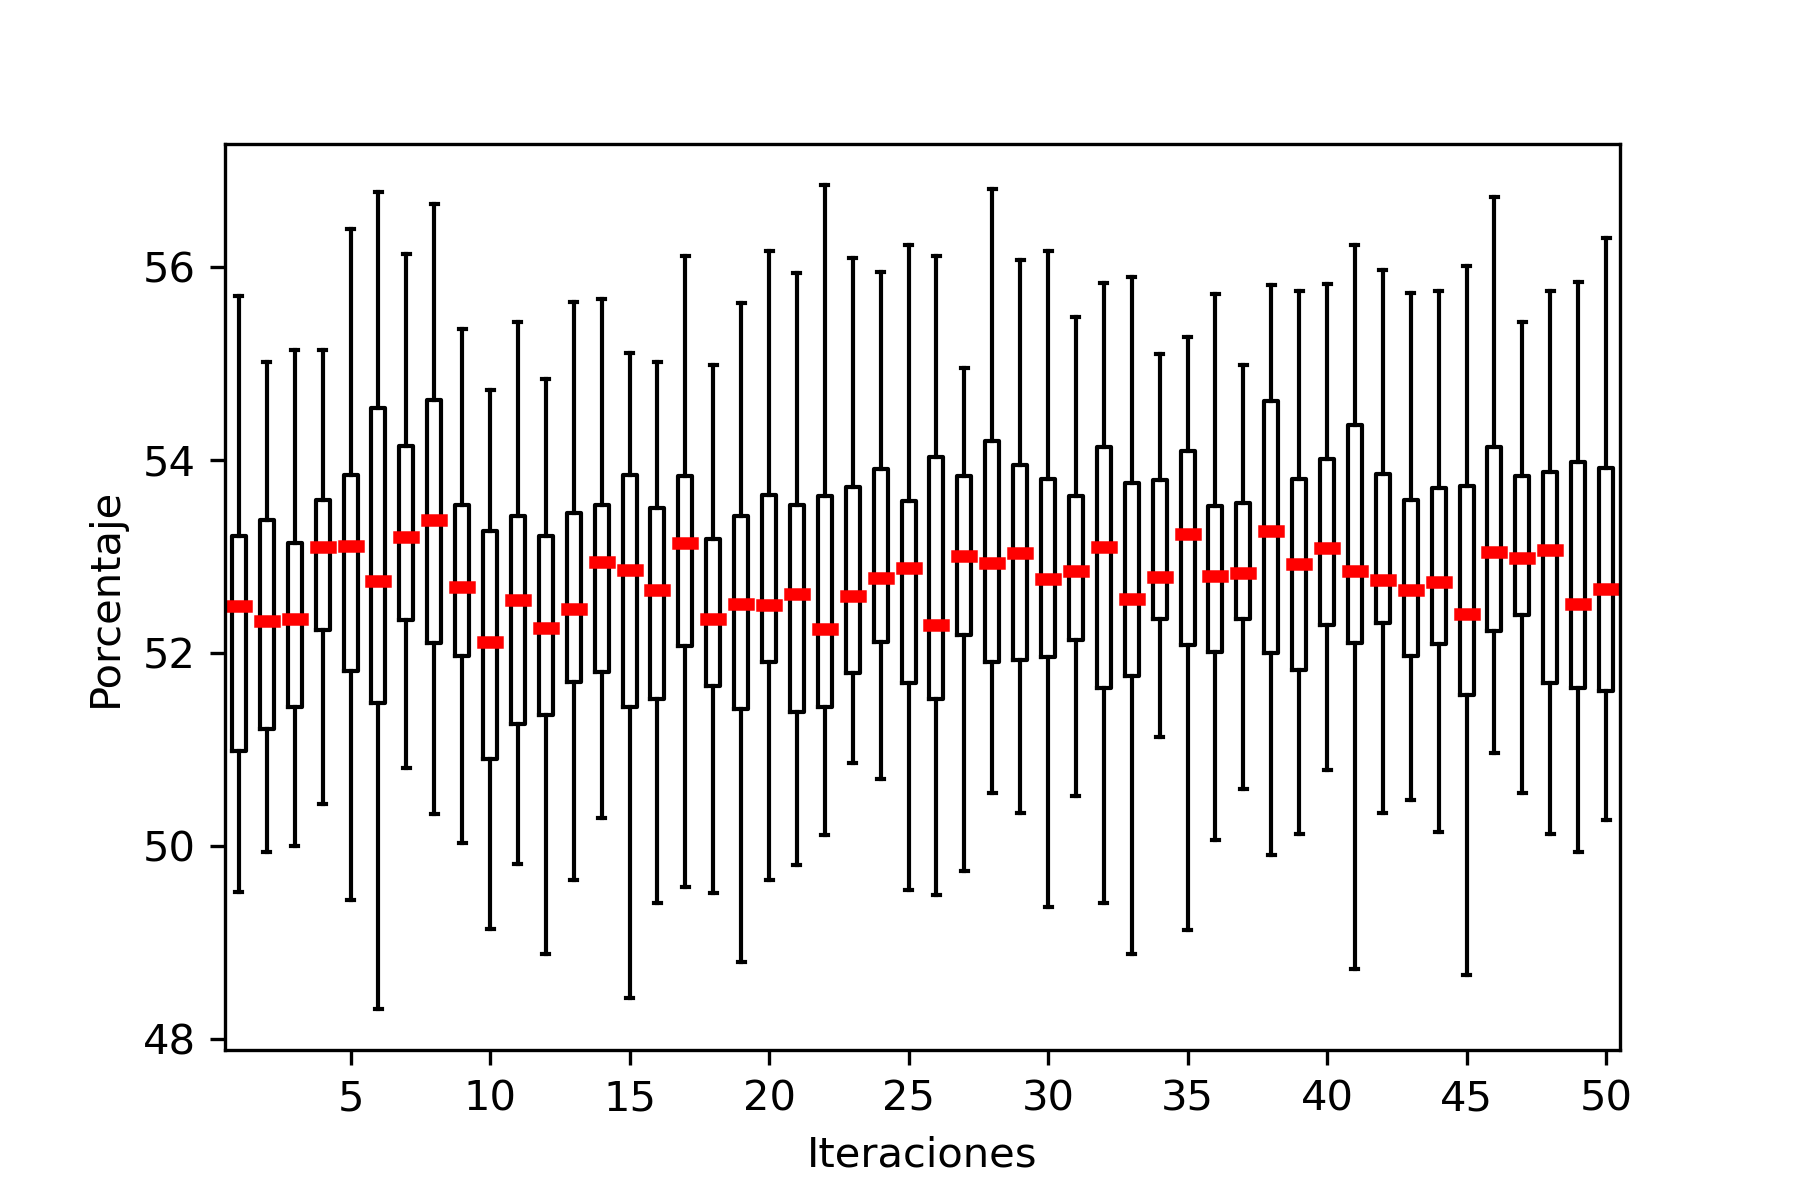
\includegraphics[width=\linewidth]{p8_n64000.png}
\caption{64000 partículas.}
\end{subfigure}
\begin{subfigure}[b]{0.40\linewidth}
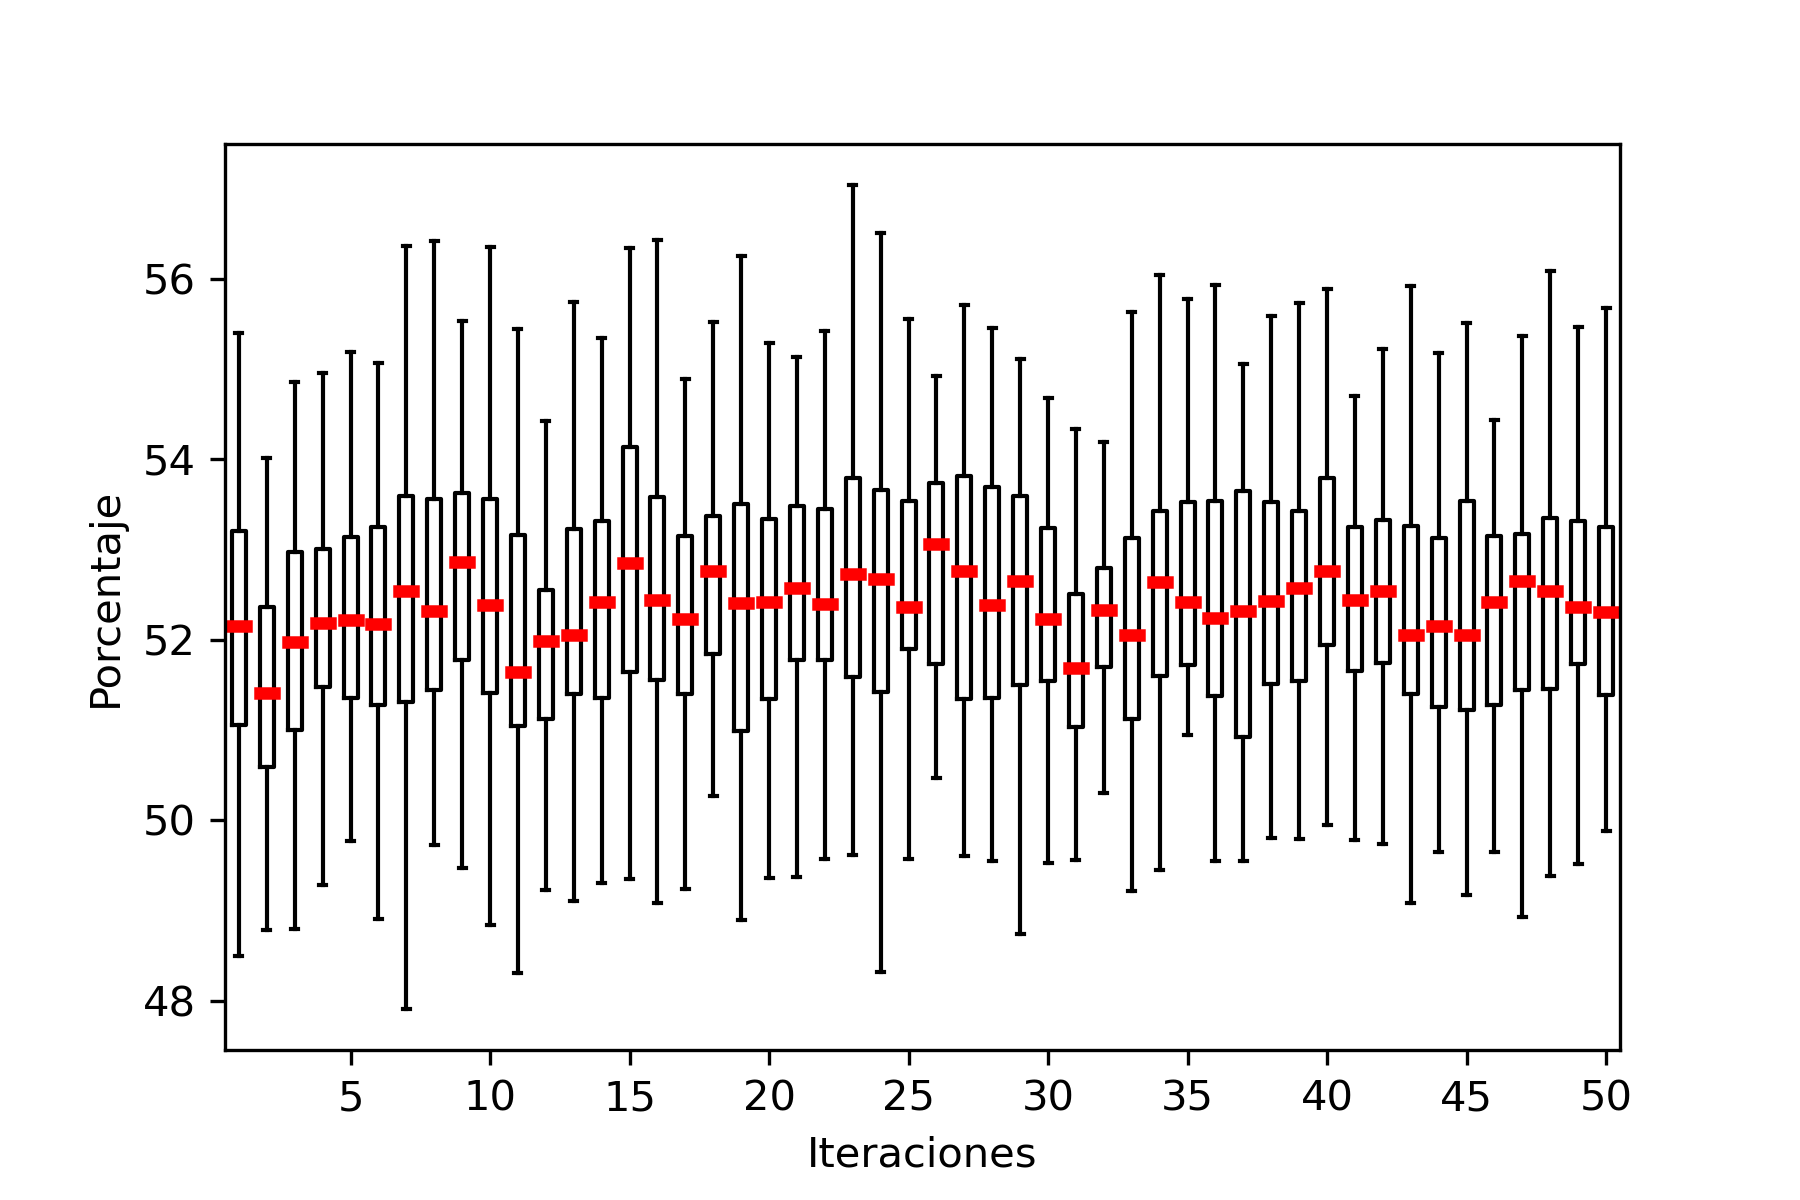
\includegraphics[width=\linewidth]{p8_n128000.png}
\caption{128000 partículas.}
\end{subfigure}
\caption{Porcentaje filtrado por iteración.}
\label{fig:westminster}
\end{figure}

\section{Reto 1}
Como primer reto, determina si hay algún intervalo de iteraciones en el que el filtrado alcance un óptimo. Realiza réplicas para determinar si el momento en el cual se alcanza el máximo tiene un comportamiento sistemático. Incluye visualizaciones para justificar las conclusiones \cite{Satu_Elisa_Schaeffer}.

Para obter las siguientes gráficas de las 50 réplicas con una duración de 50 pasps se repitieron 25 veces para de ahí sacar la mejor mediana por repetición. 
En el cuadro 1 se muestra el porcentaje de la iteración que más se repite. El código completo se encuentra en GitHub \cite{Denisse_Leyva}.

\begin{figure}[H]
\centering
\begin{subfigure}[b]{0.40\linewidth}
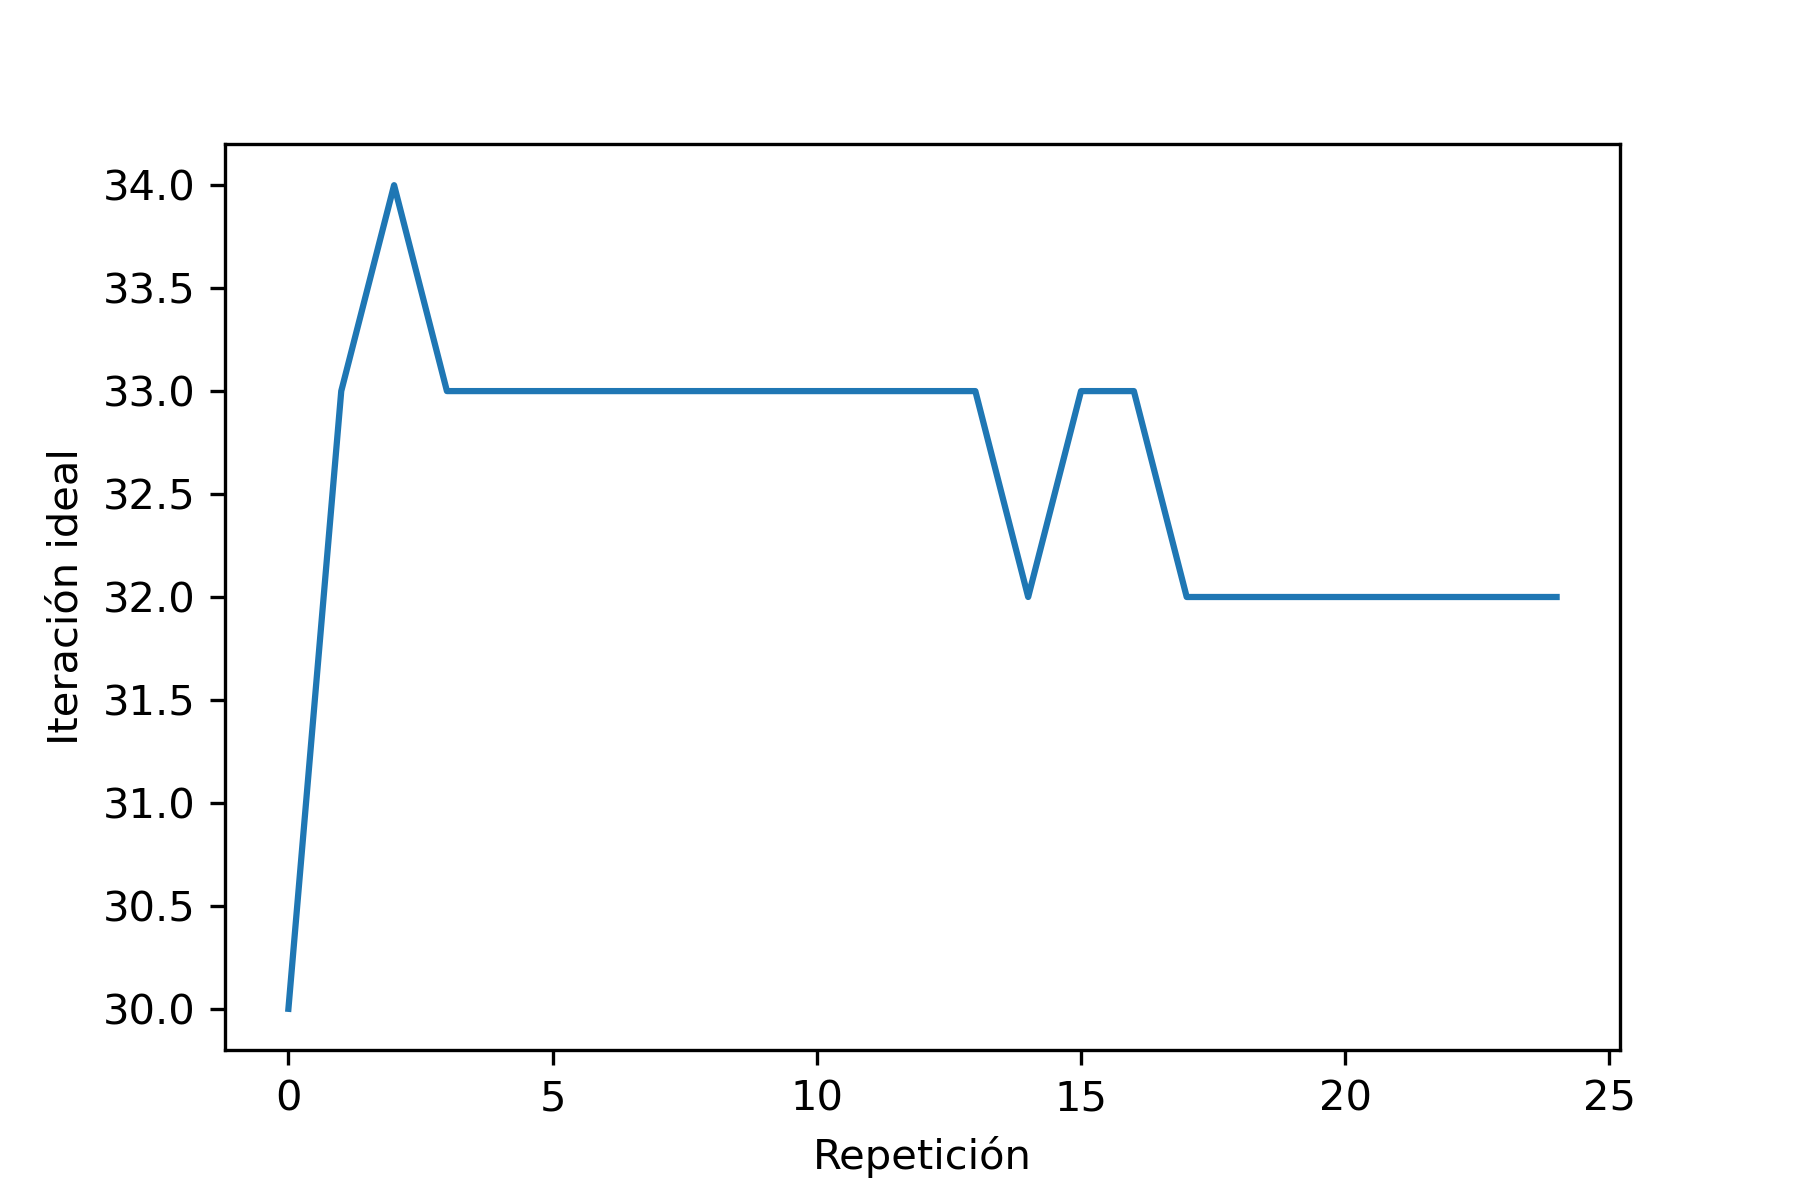
\includegraphics[width=\linewidth]{p8_r1_n16000.png}
\caption{16000 partículas.}
\end{subfigure}
\begin{subfigure}[b]{0.40\linewidth}
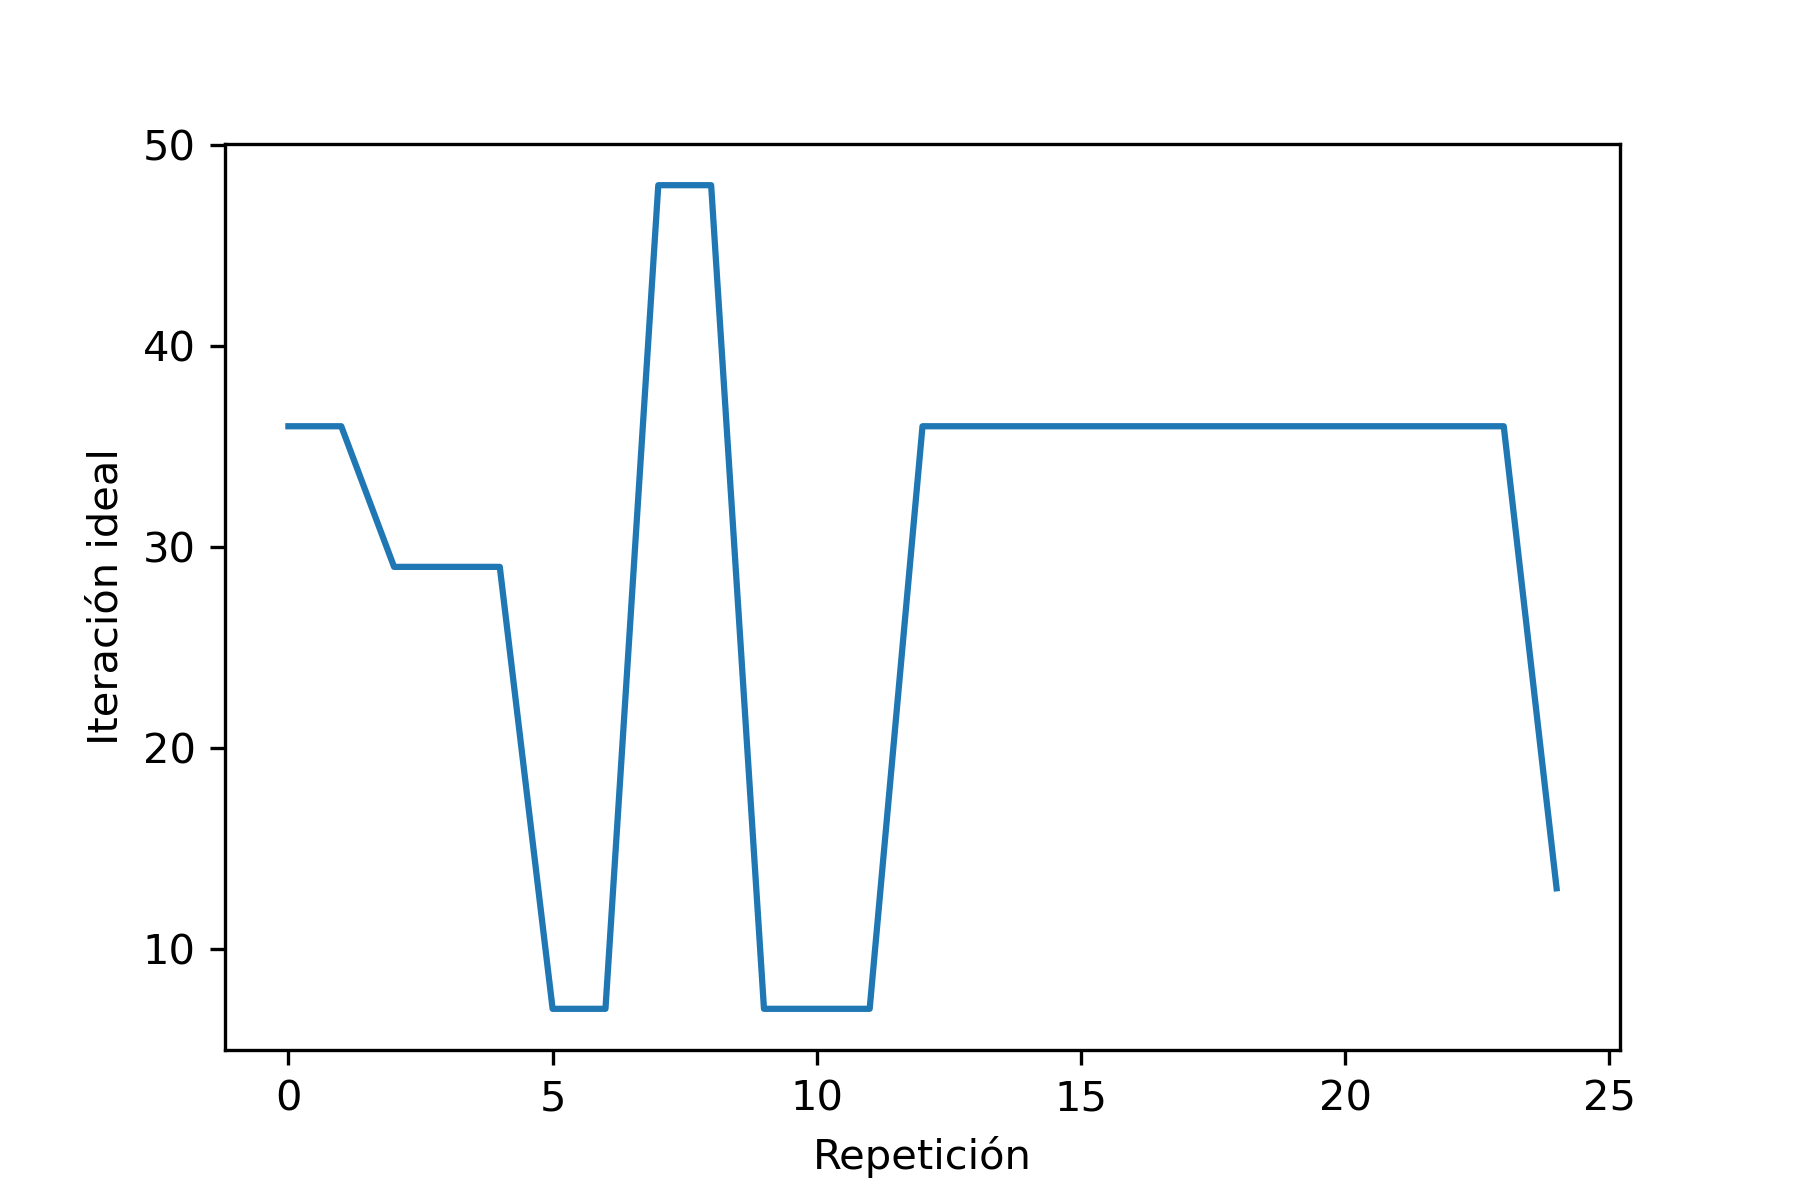
\includegraphics[width=\linewidth]{p8_r1_n32000.png}
\caption{32000 partículas.}
\end{subfigure}
\caption{Gráfica de iteración ideal por repetición.}
\label{fig:westminster}
\end{figure}

\begin{figure}[H]
\centering
\begin{subfigure}[b]{0.40\linewidth}
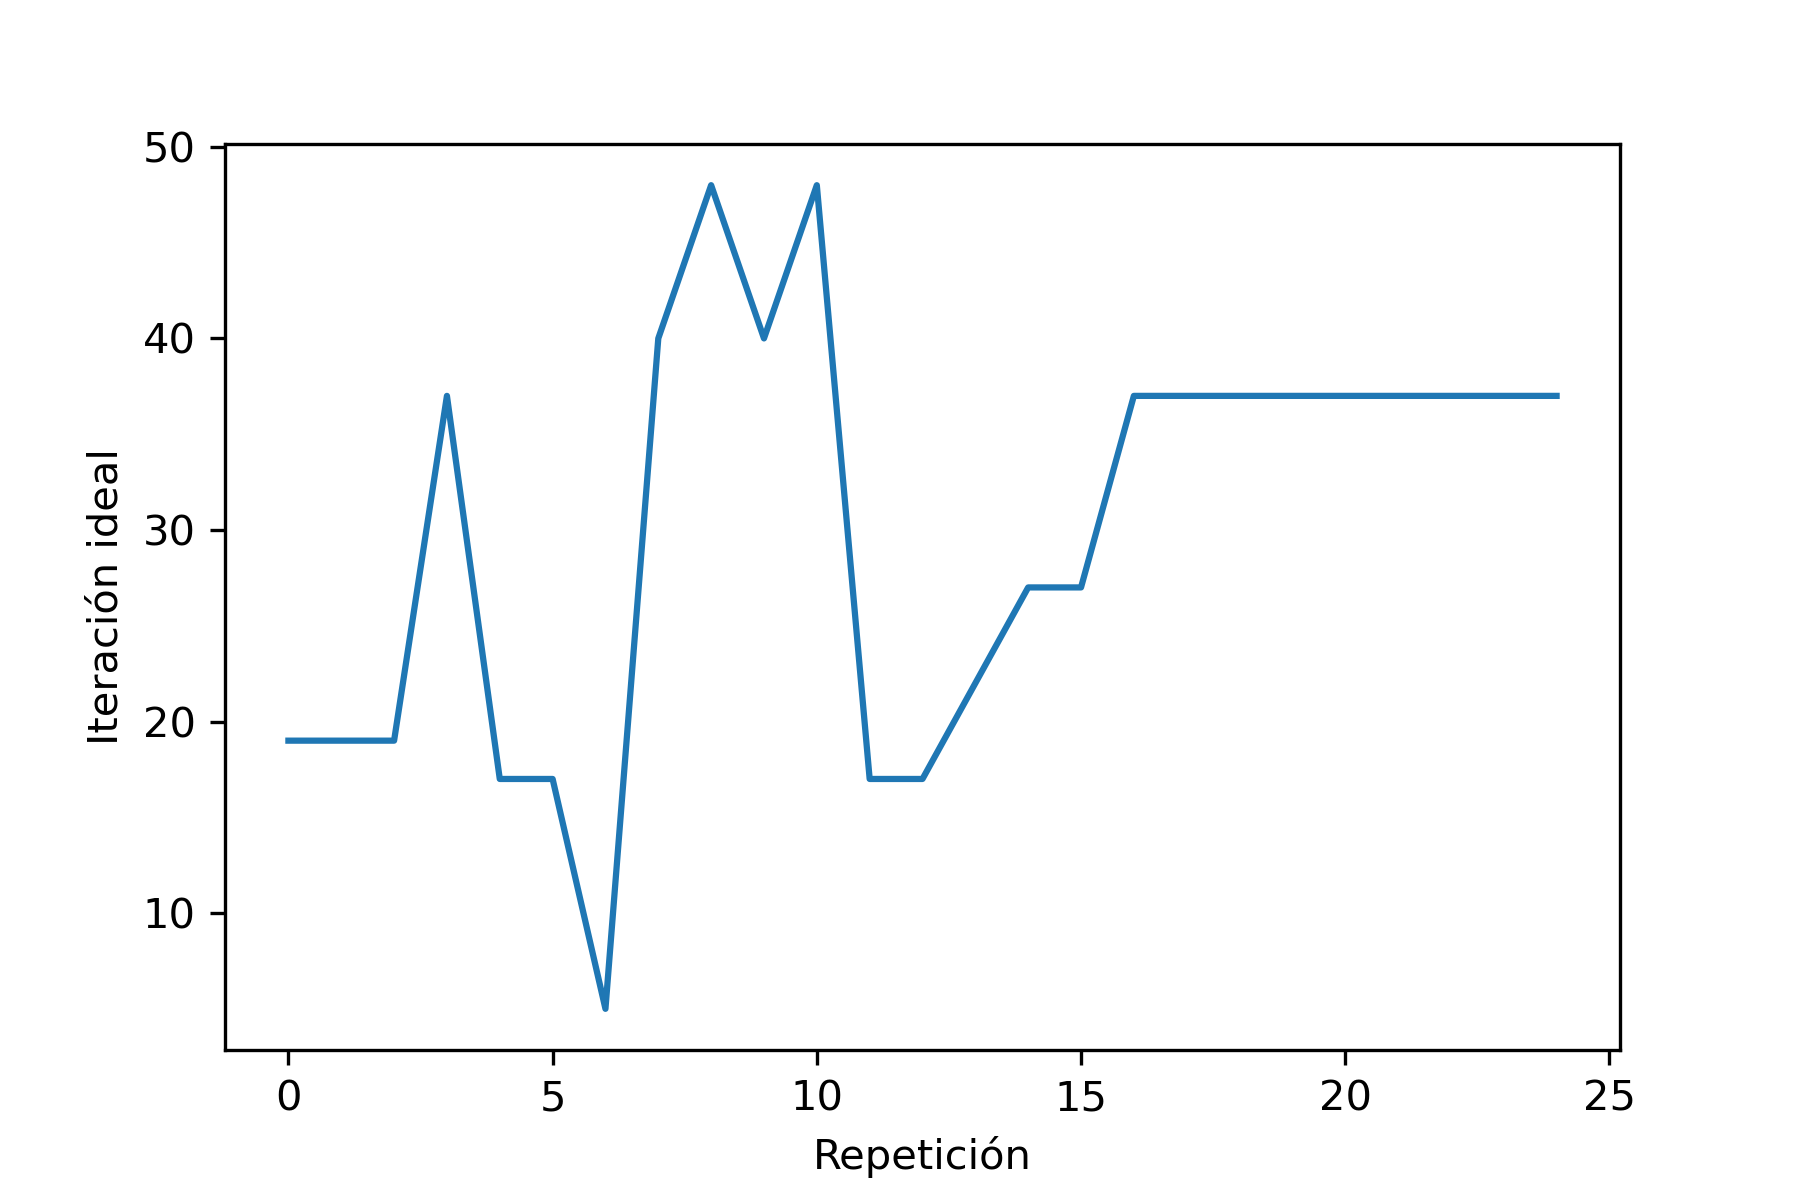
\includegraphics[width=\linewidth]{p8_r1_n64000.png}
\caption{64000 partículas.}
\end{subfigure}
\begin{subfigure}[b]{0.40\linewidth}
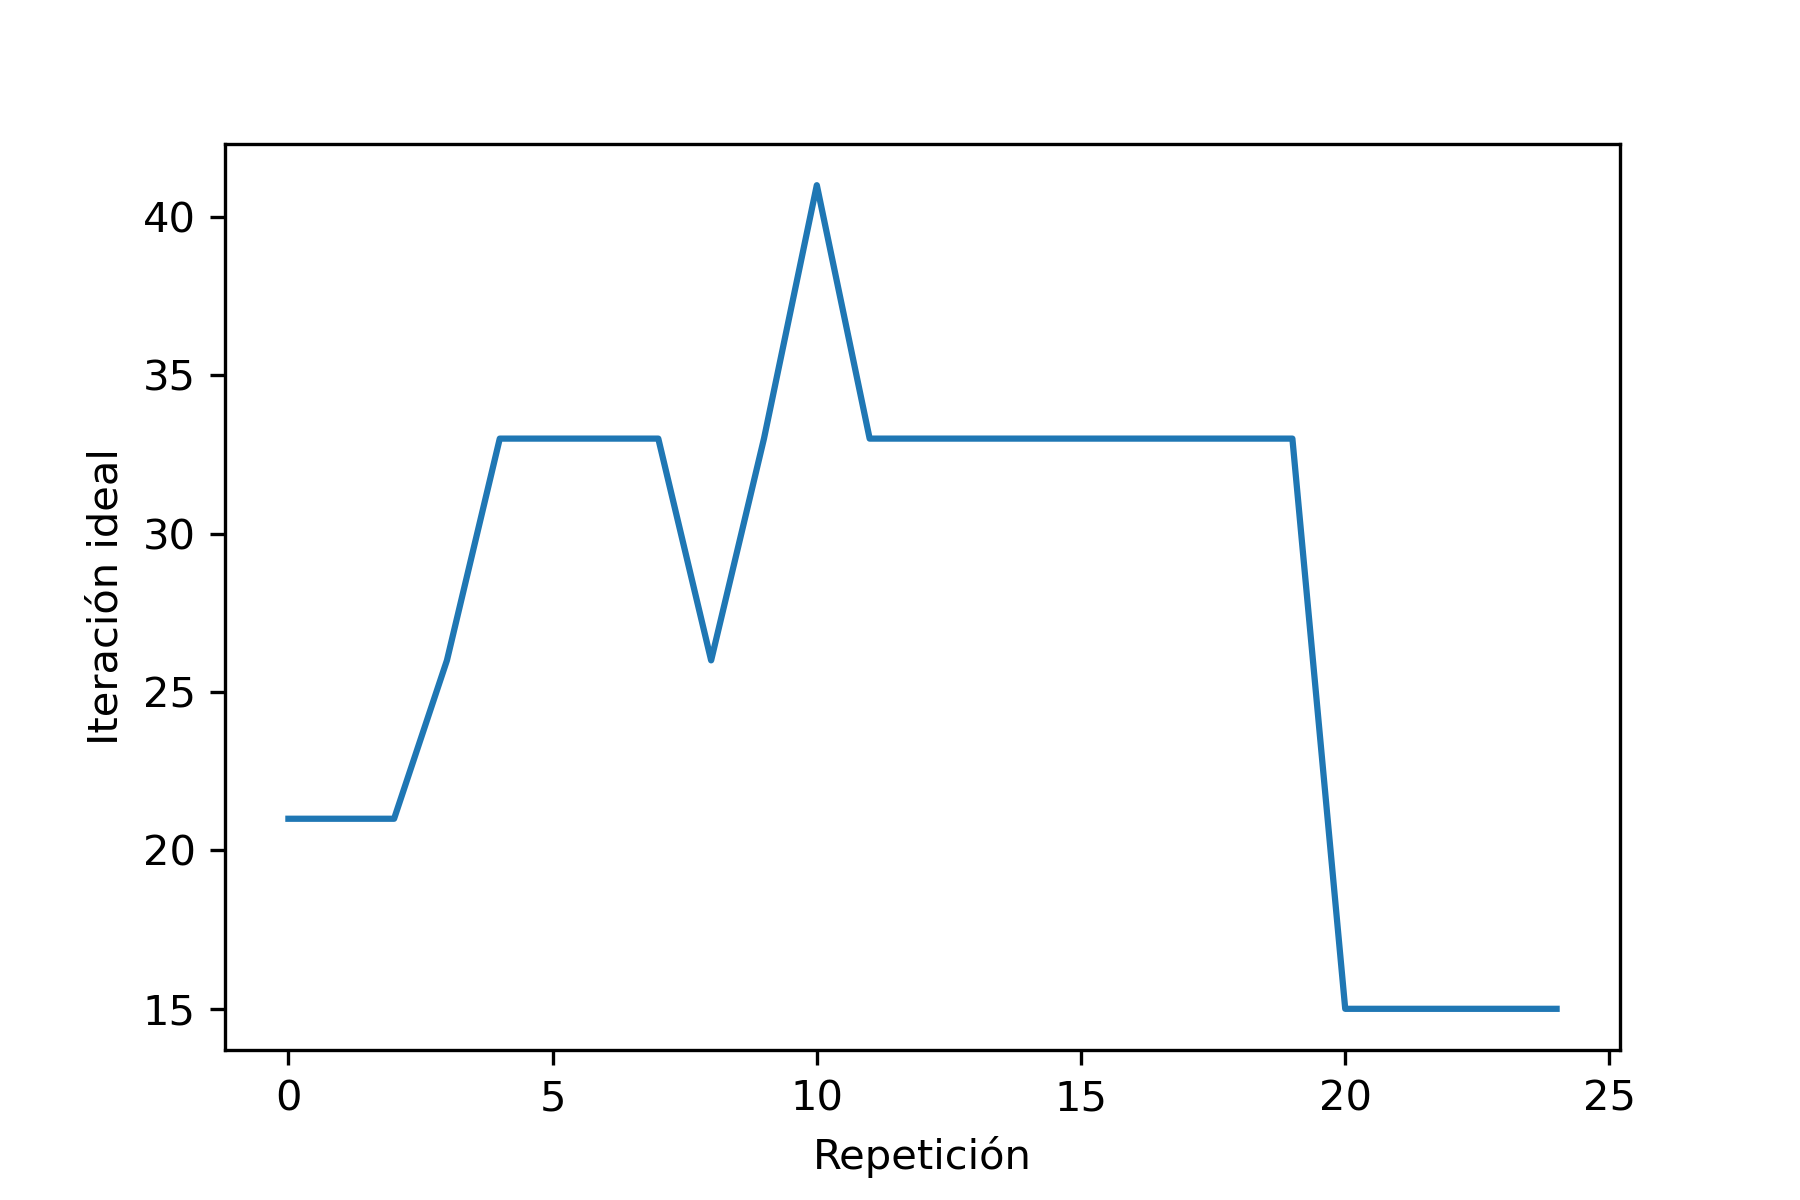
\includegraphics[width=\linewidth]{p8_r1_n128000.png}
\caption{128000 partículas.}
\end{subfigure}
\caption{Gráfica de iteración ideal por repetición.}
\label{fig:westminster}
\end{figure}

\begin{figure}[H]
\centering
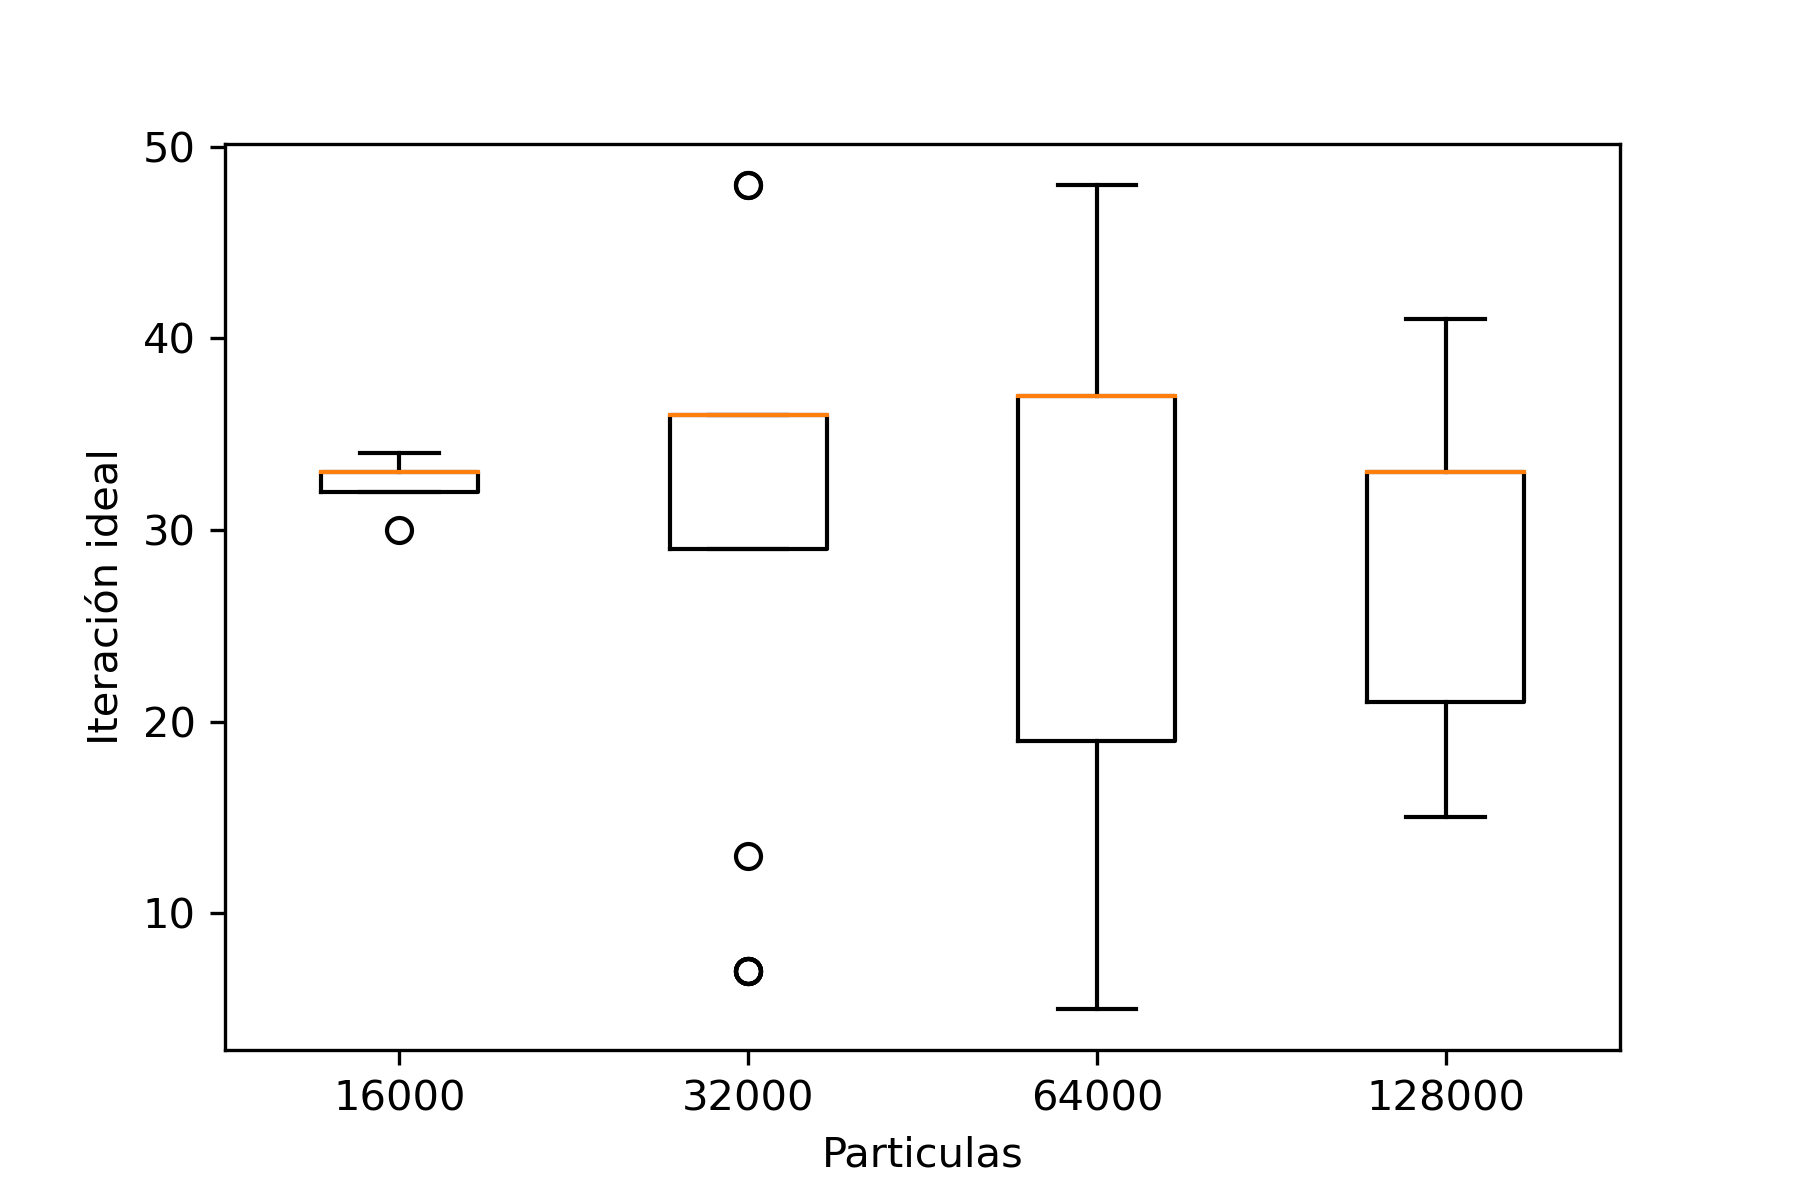
\includegraphics[width=80mm]{p8_01_r1_n128000.png}
\caption{\label{fig3} Gráfica caja bigote de iteración ideal.}
\end{figure}

\begin{table}[h!]
\centering
\caption{Porcentaje de la mejor iteración para filtrar.}
 \begin{tabular}{||r r r||} 
 \hline
 Partículas & Valor Ideal & Porcentaje  \\ [0.5ex] 
 \hline\hline
 16000 & 33 & 56\% \\
 \hline
 32000 & 36 & 56\%\\ 
 \hline
 64000 & 37 & 40\%  \\
 \hline
 128000 & 33 & 56\% \\
 \hline
\end{tabular}
\label{table:1}
\end{table}

\section{Reto 2}
Como un segundo reto, determina cómo los resultados de la tarea y del primer reto dependen del valor de $c$ . ¿Qué todo cambia y cómo si $c$ ya no se asigna como la mediana inicial sino a un valor menor o mayor? \cite{Satu_Elisa_Schaeffer}.

\begin{figure}[H]
\centering
\begin{subfigure}[b]{0.40\linewidth}
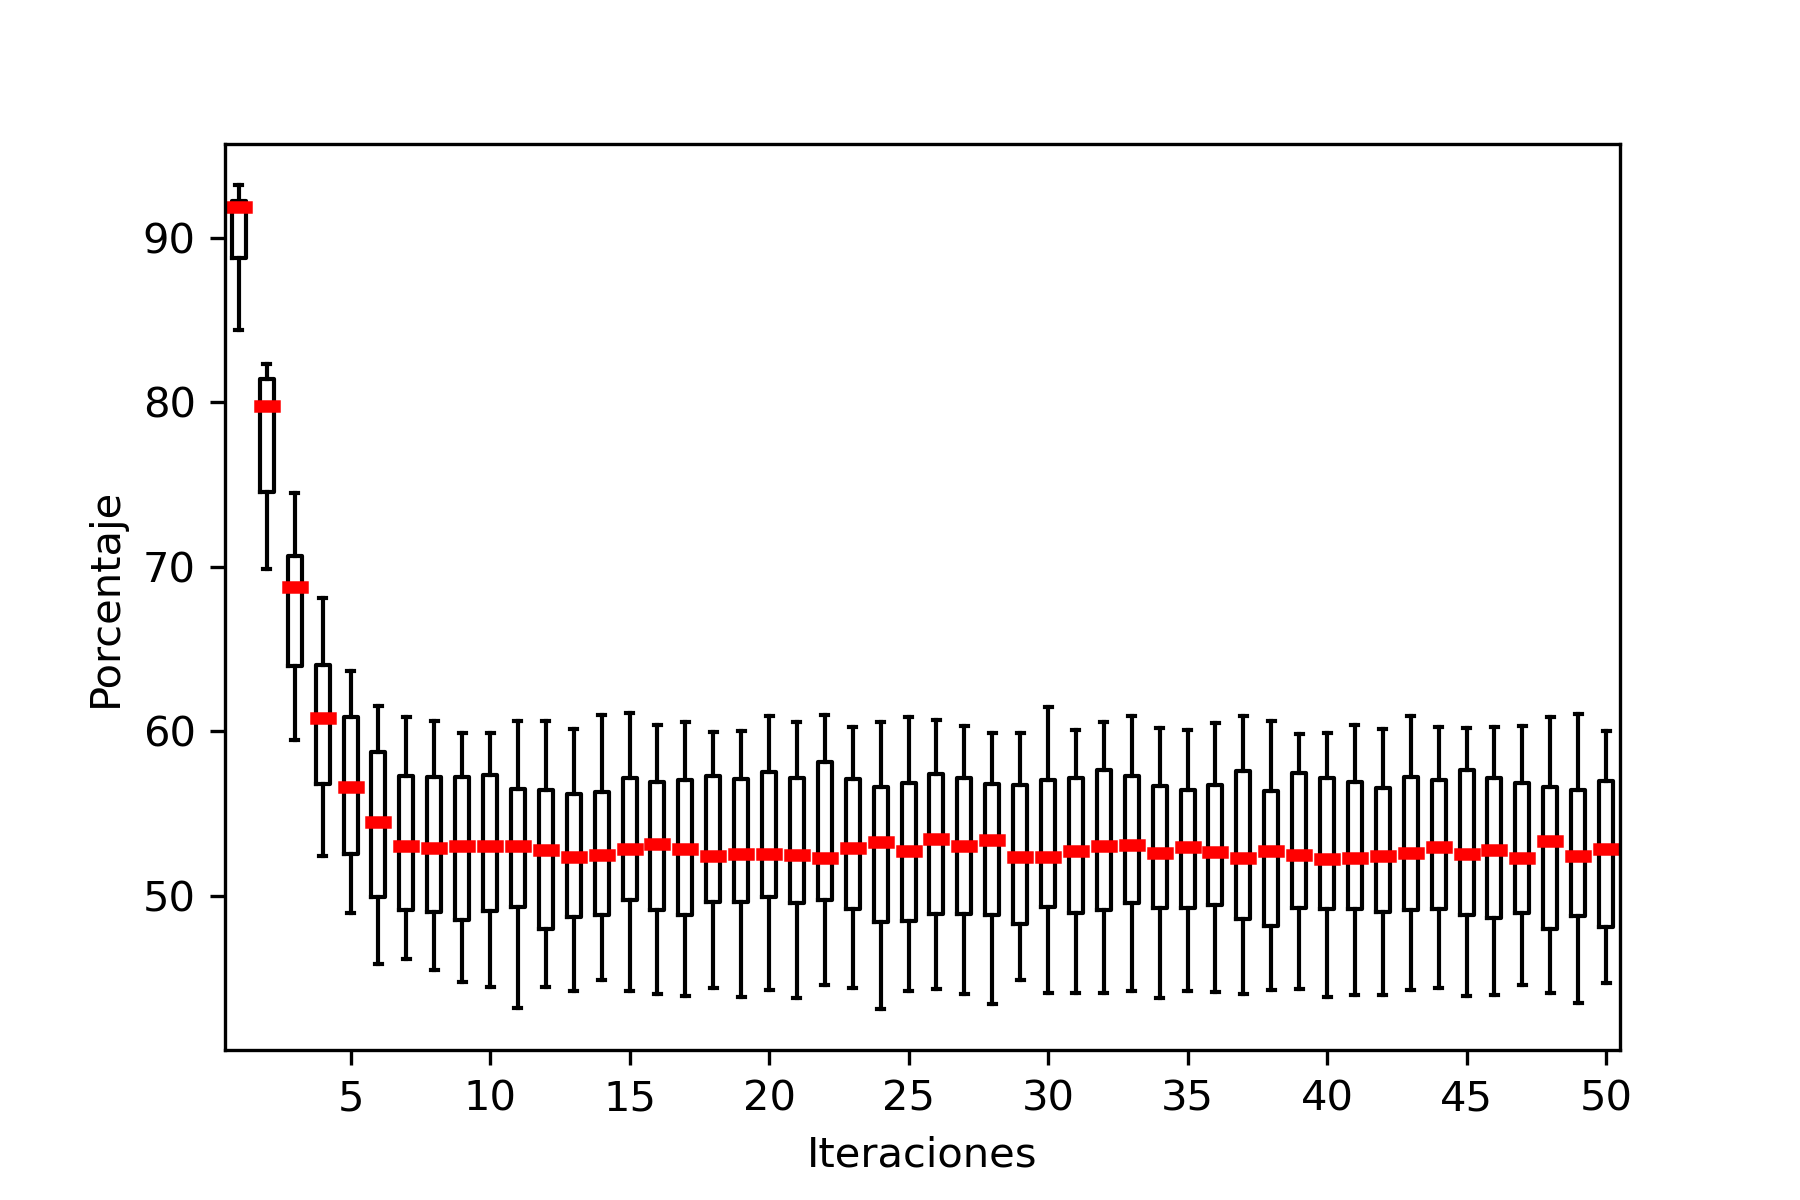
\includegraphics[width=\linewidth]{p8_v1_c1_n16000.png}
\caption{16000 partículas en c1.}
\end{subfigure}
\begin{subfigure}[b]{0.40\linewidth}
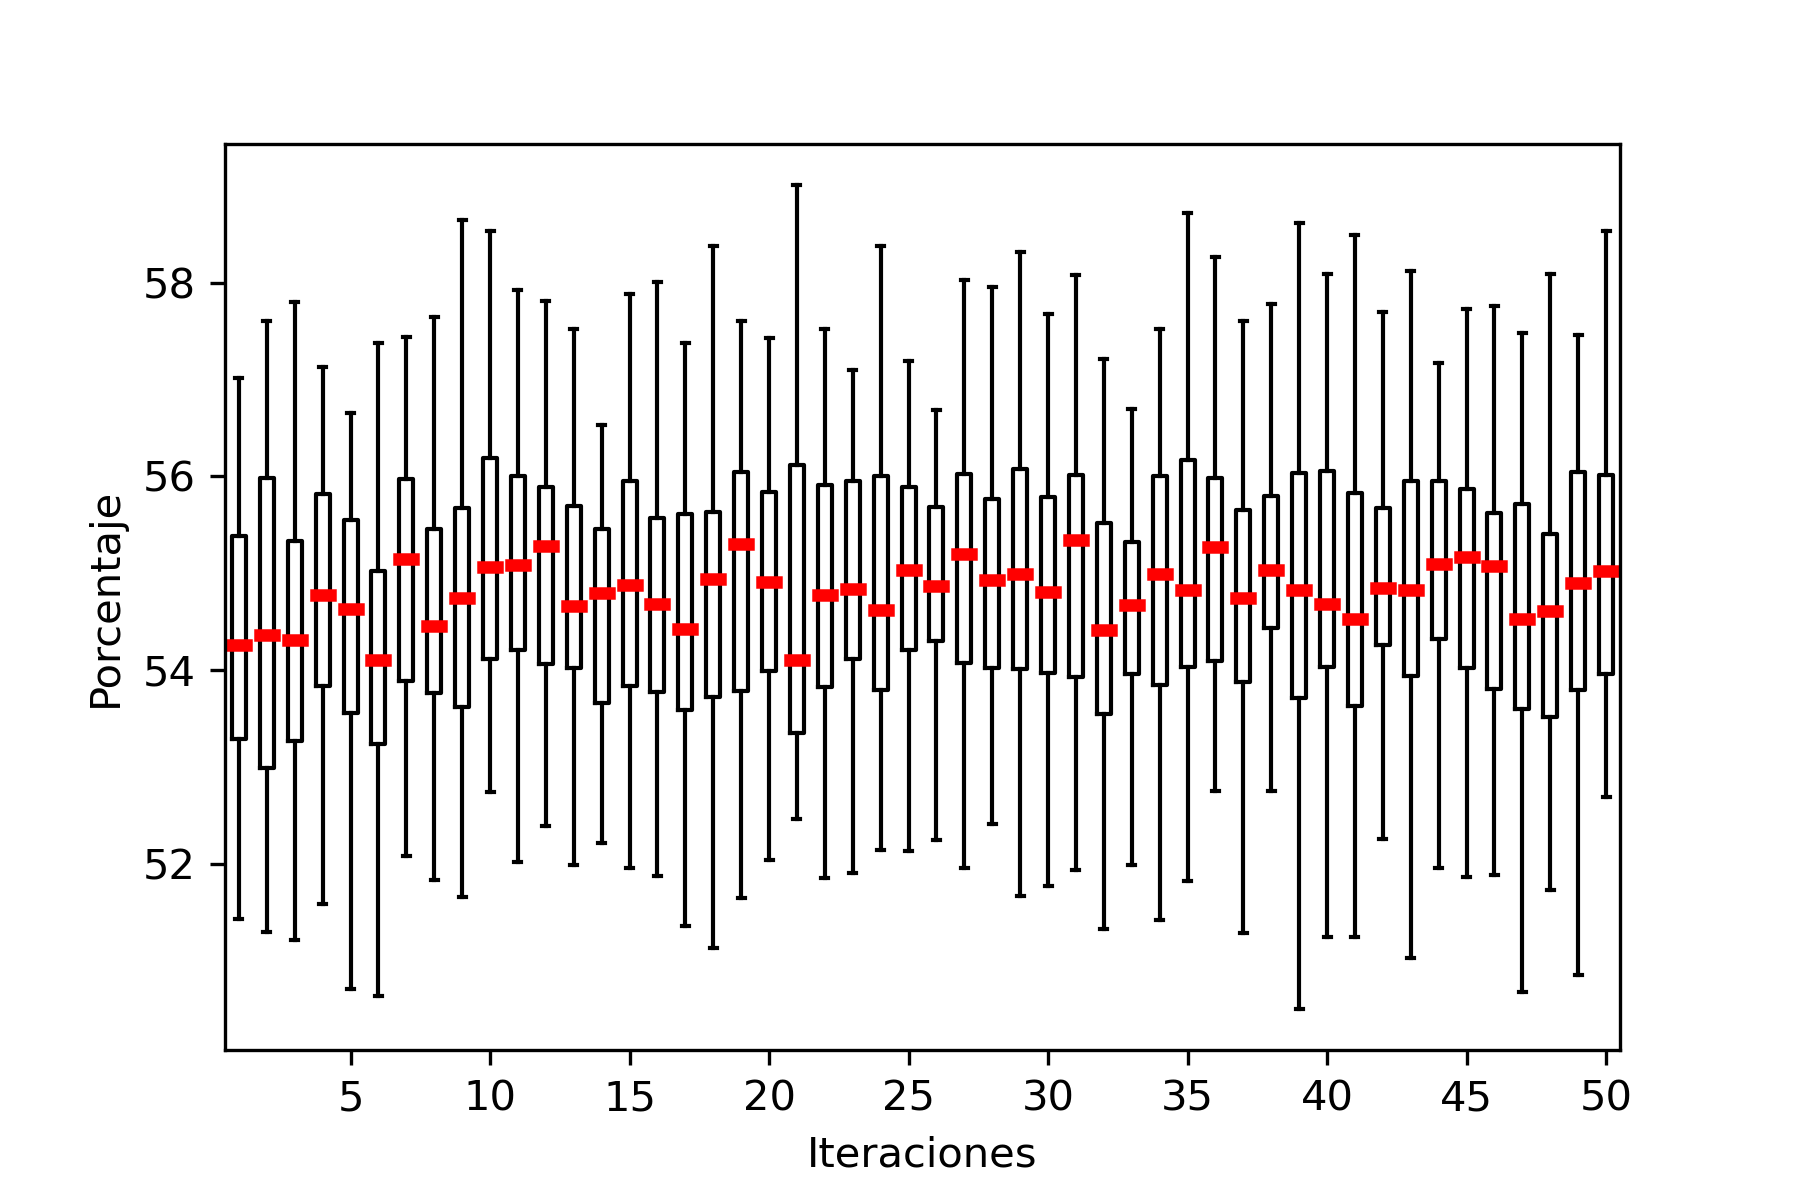
\includegraphics[width=\linewidth]{p8_v1_c2_n16000.png}
\caption{16000 partículas en c2.}
\end{subfigure}
\caption{Gráficas de porcentaje en diferentes puntos críticos.}
\label{fig:westminster}
\end{figure}

\begin{figure}[H]
\centering
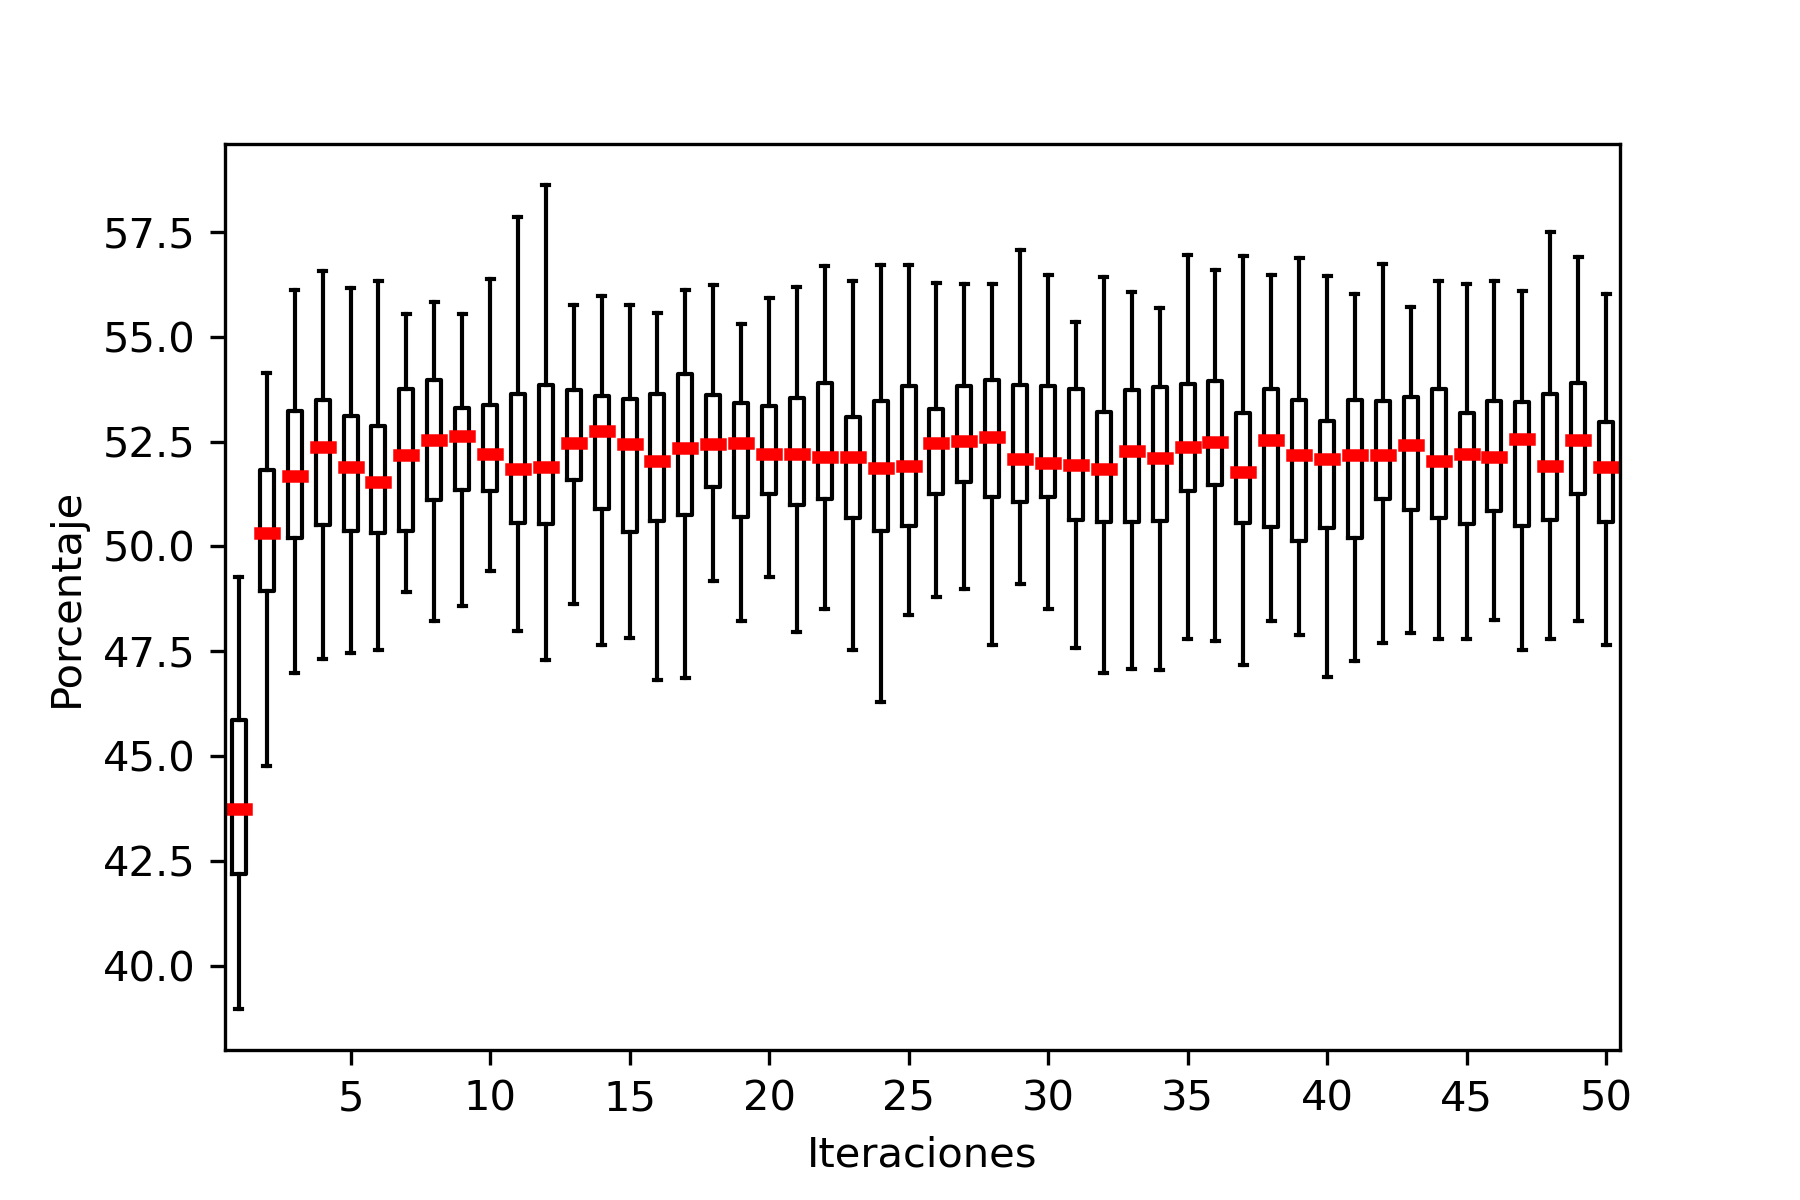
\includegraphics[width=80mm]{p8_v1_c3_n16000.png}
\caption{\label{fig3} 16000 partículas en c3.}
\end{figure}

\begin{figure}[H]
\centering
\begin{subfigure}[b]{0.40\linewidth}
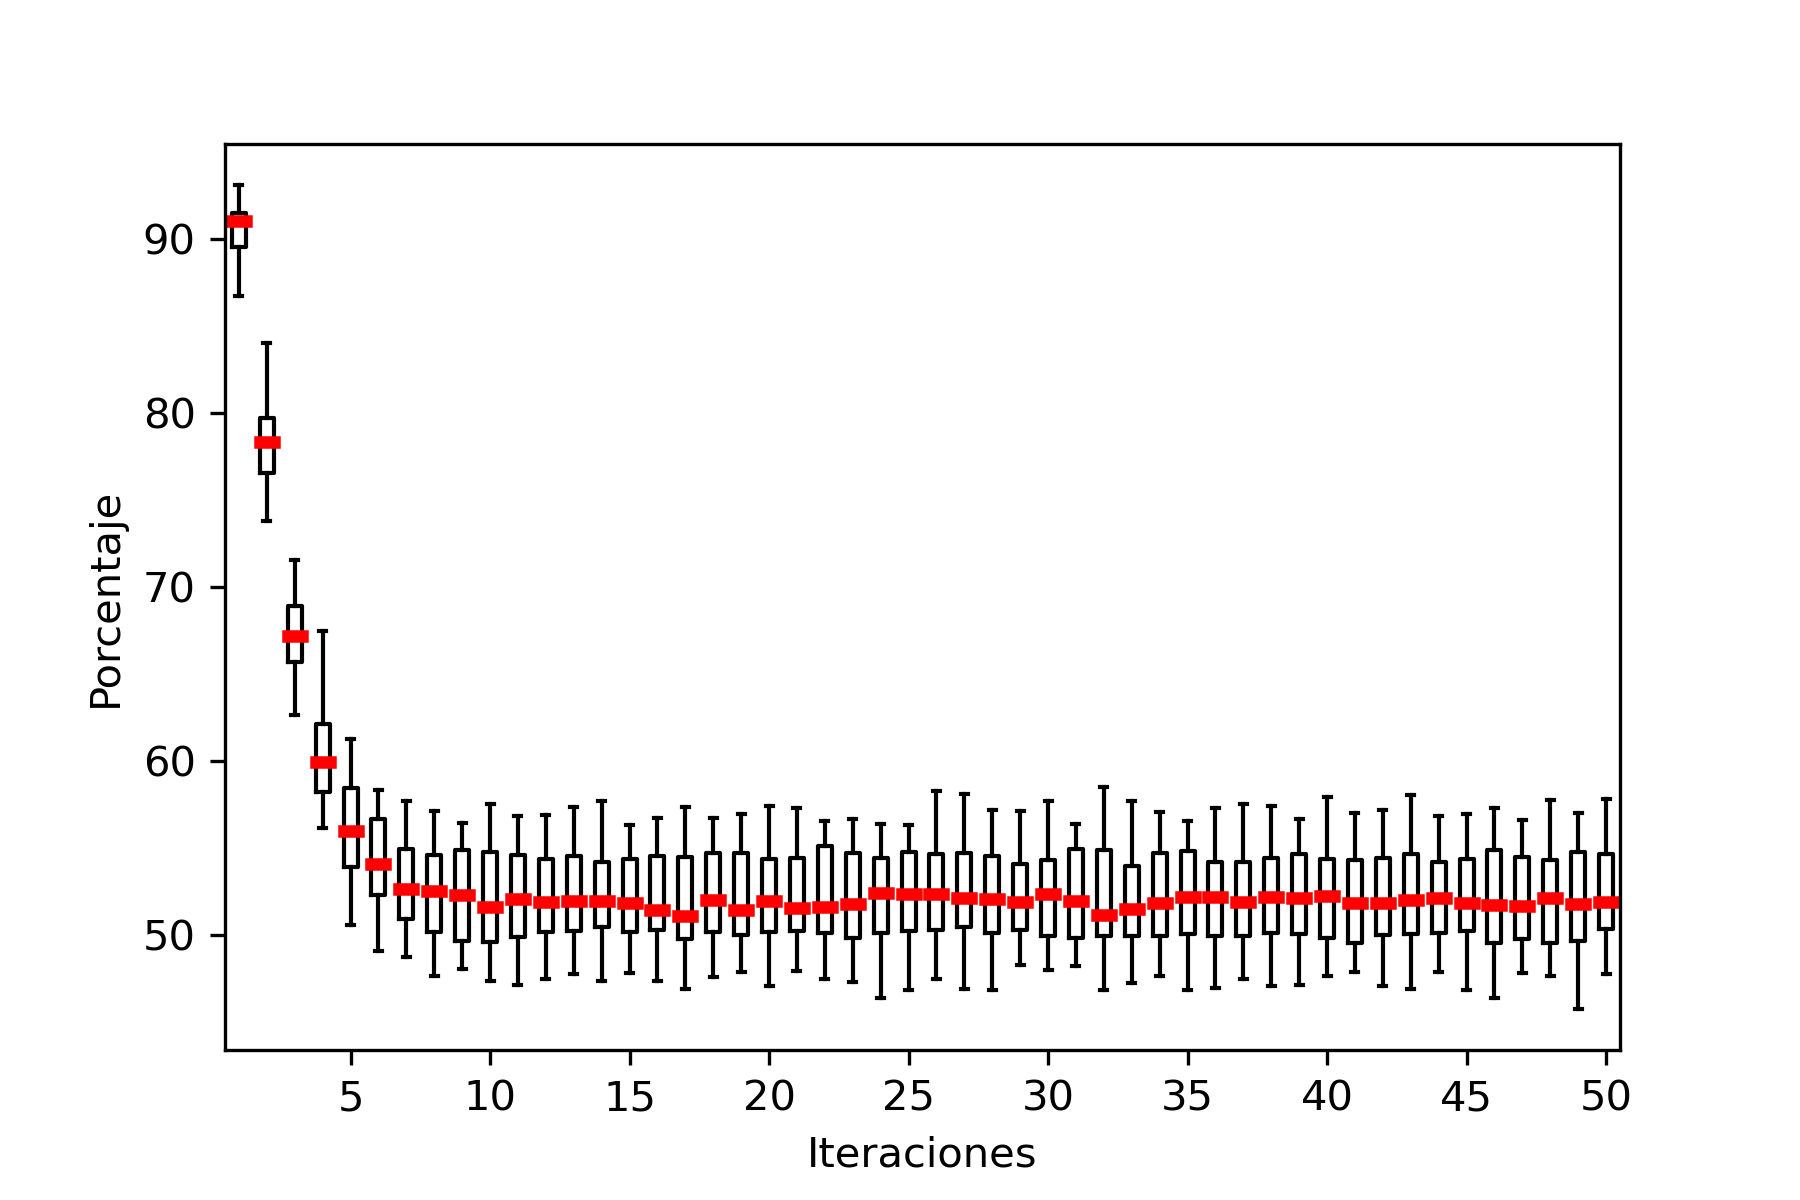
\includegraphics[width=\linewidth]{p8_v1_c1_n32000.png}
\caption{32000 partículas en c1.}
\end{subfigure}
\begin{subfigure}[b]{0.40\linewidth}
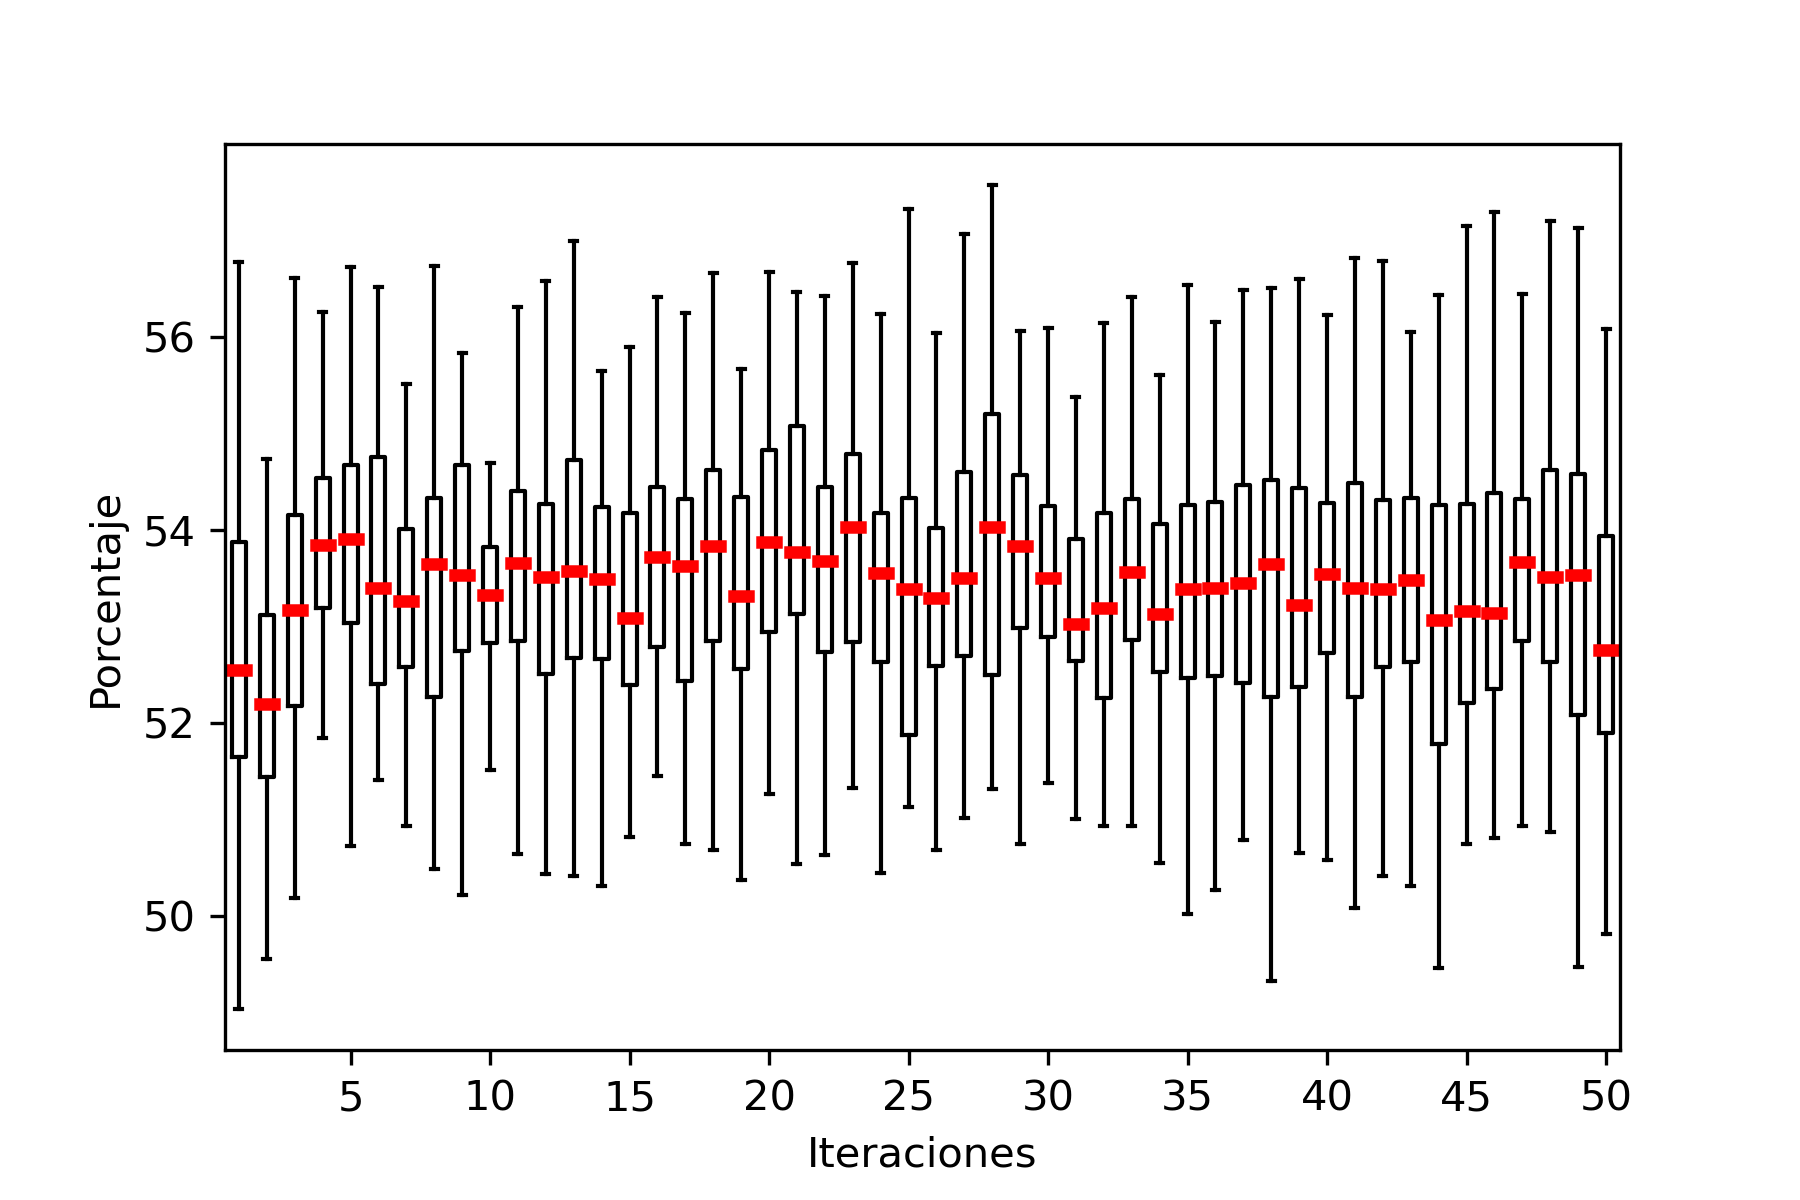
\includegraphics[width=\linewidth]{p8_v1_c2_n32000.png}
\caption{32000 partículas en c2.}
\end{subfigure}
\caption{Gráficas de porcentaje en diferentes puntos críticos.}
\label{fig:westminster}
\end{figure}

\begin{figure}[H]
\centering
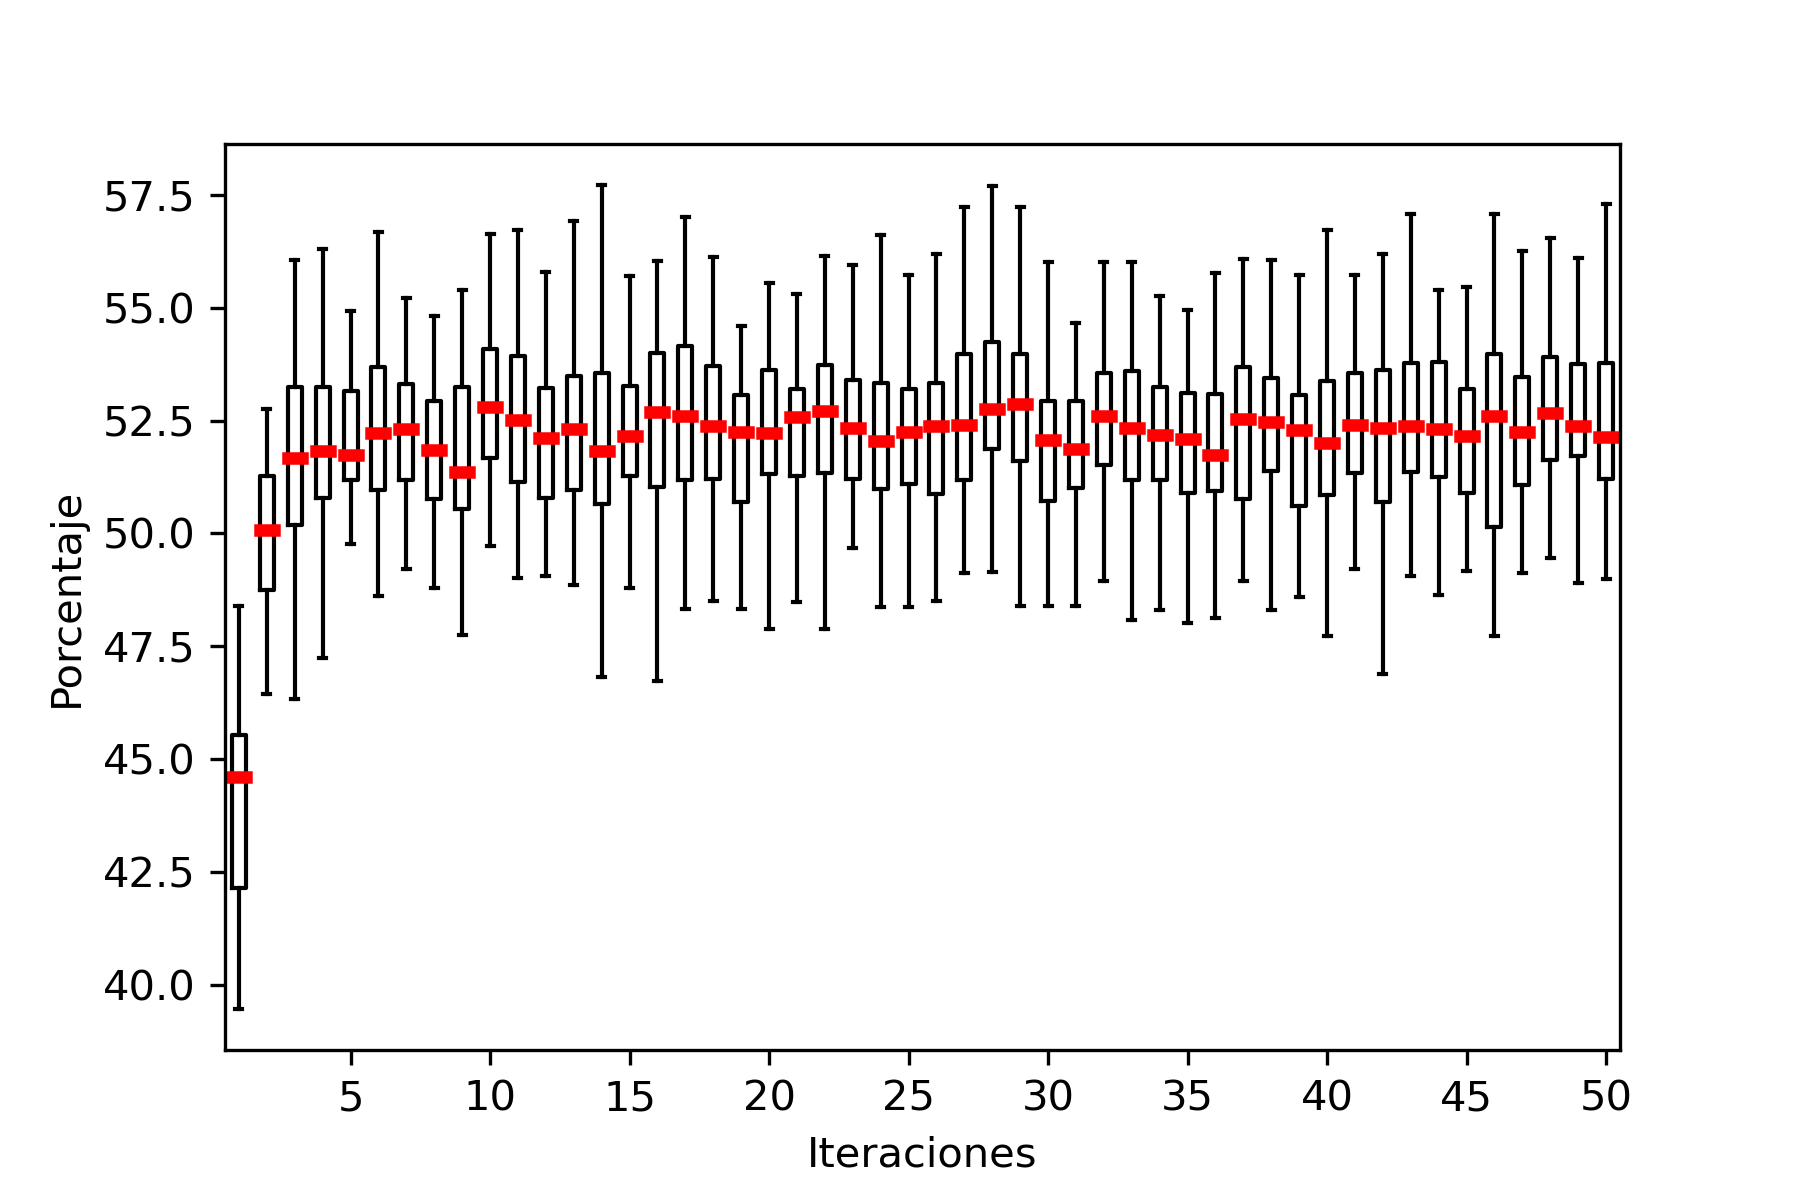
\includegraphics[width=80mm]{p8_v1_c3_n32000.png}
\caption{\label{fig3} 32000 partículas en c3.}
\end{figure}

\begin{figure}[H]
\centering
\begin{subfigure}[b]{0.40\linewidth}
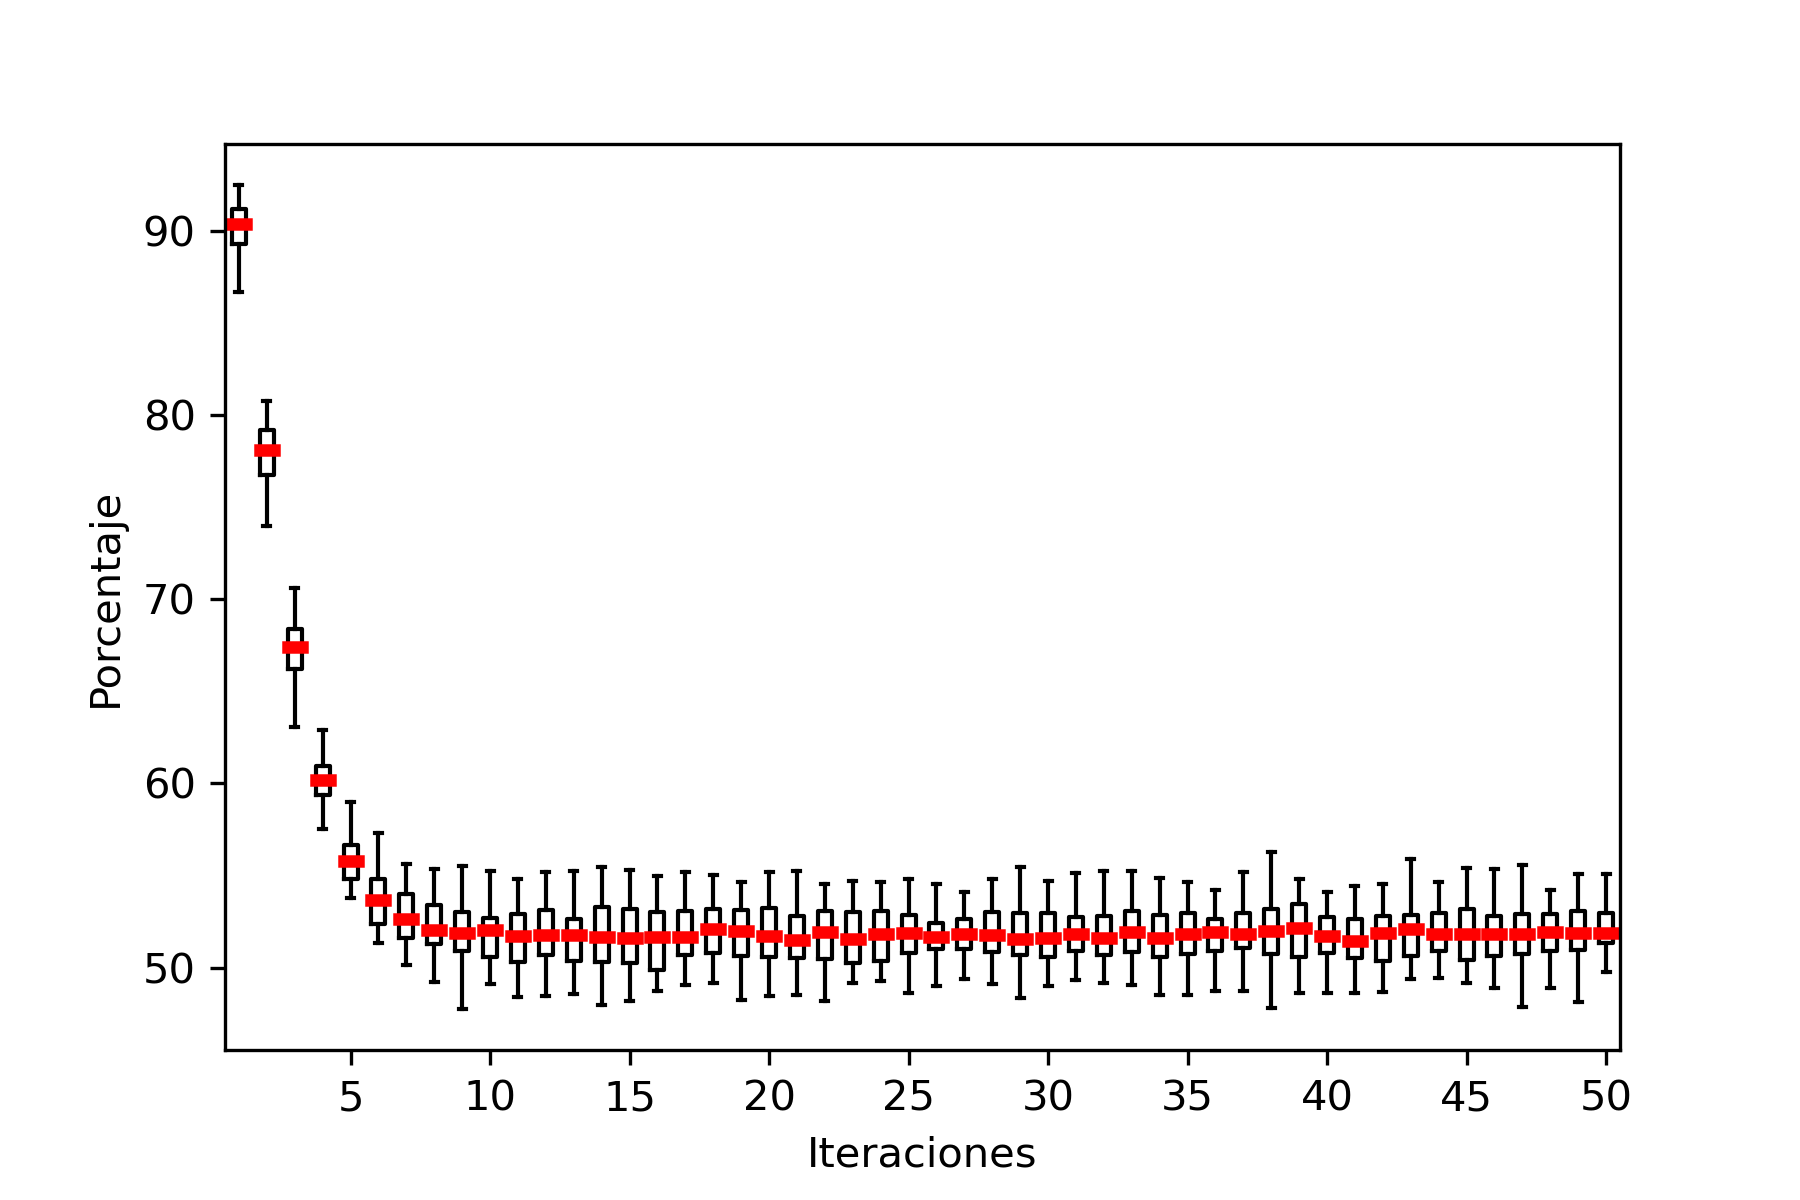
\includegraphics[width=\linewidth]{p8_v1_c1_n64000.png}
\caption{64000 partículas en c1.}
\end{subfigure}
\begin{subfigure}[b]{0.40\linewidth}
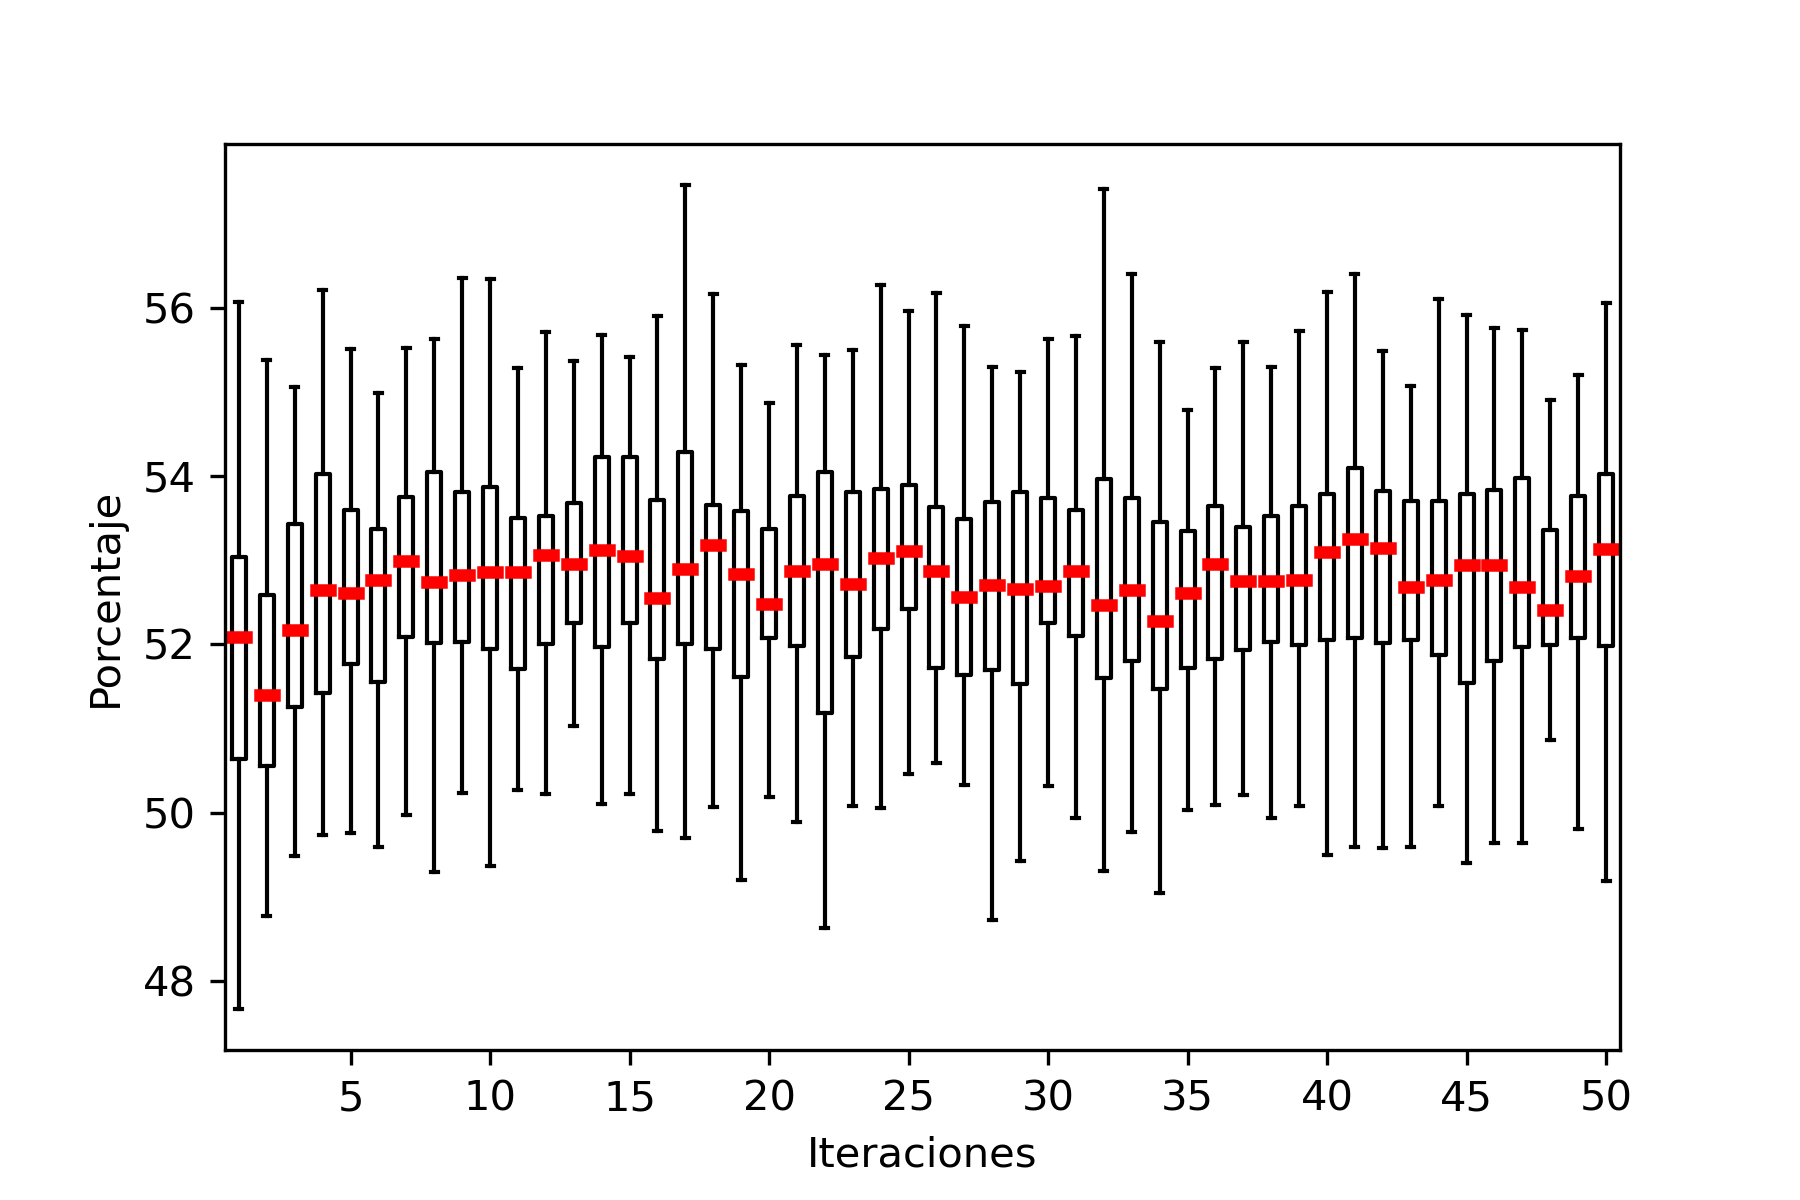
\includegraphics[width=\linewidth]{p8_v1_c2_n64000.png}
\caption{64000 partículas en c2.}
\end{subfigure}
\caption{Gráficas de porcentaje en diferentes puntos críticos.}
\label{fig:westminster}
\end{figure}

\begin{figure}[H]
\centering
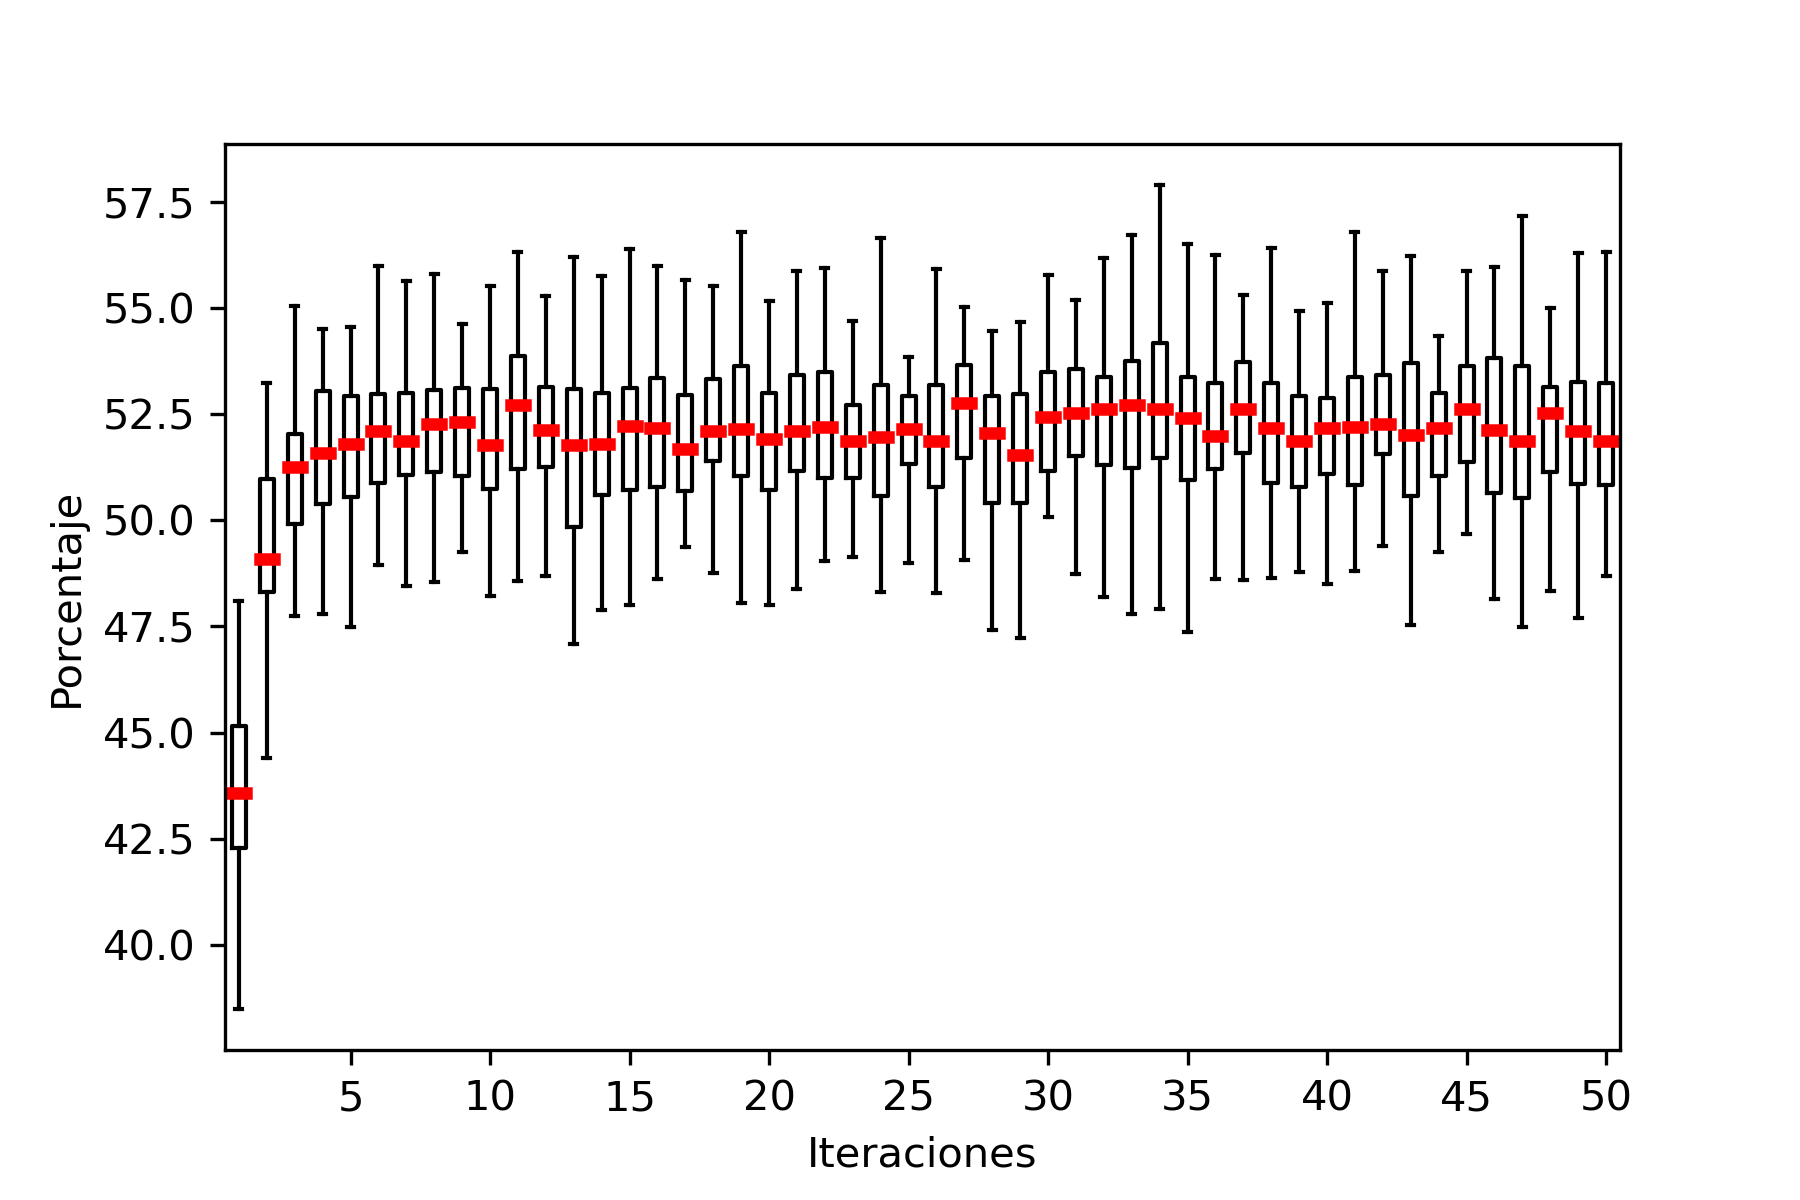
\includegraphics[width=80mm]{p8_v1_c3_n64000.png}
\caption{\label{fig3} 64000 partículas en c3.}
\end{figure}

\begin{figure}[H]
\centering
\begin{subfigure}[b]{0.40\linewidth}
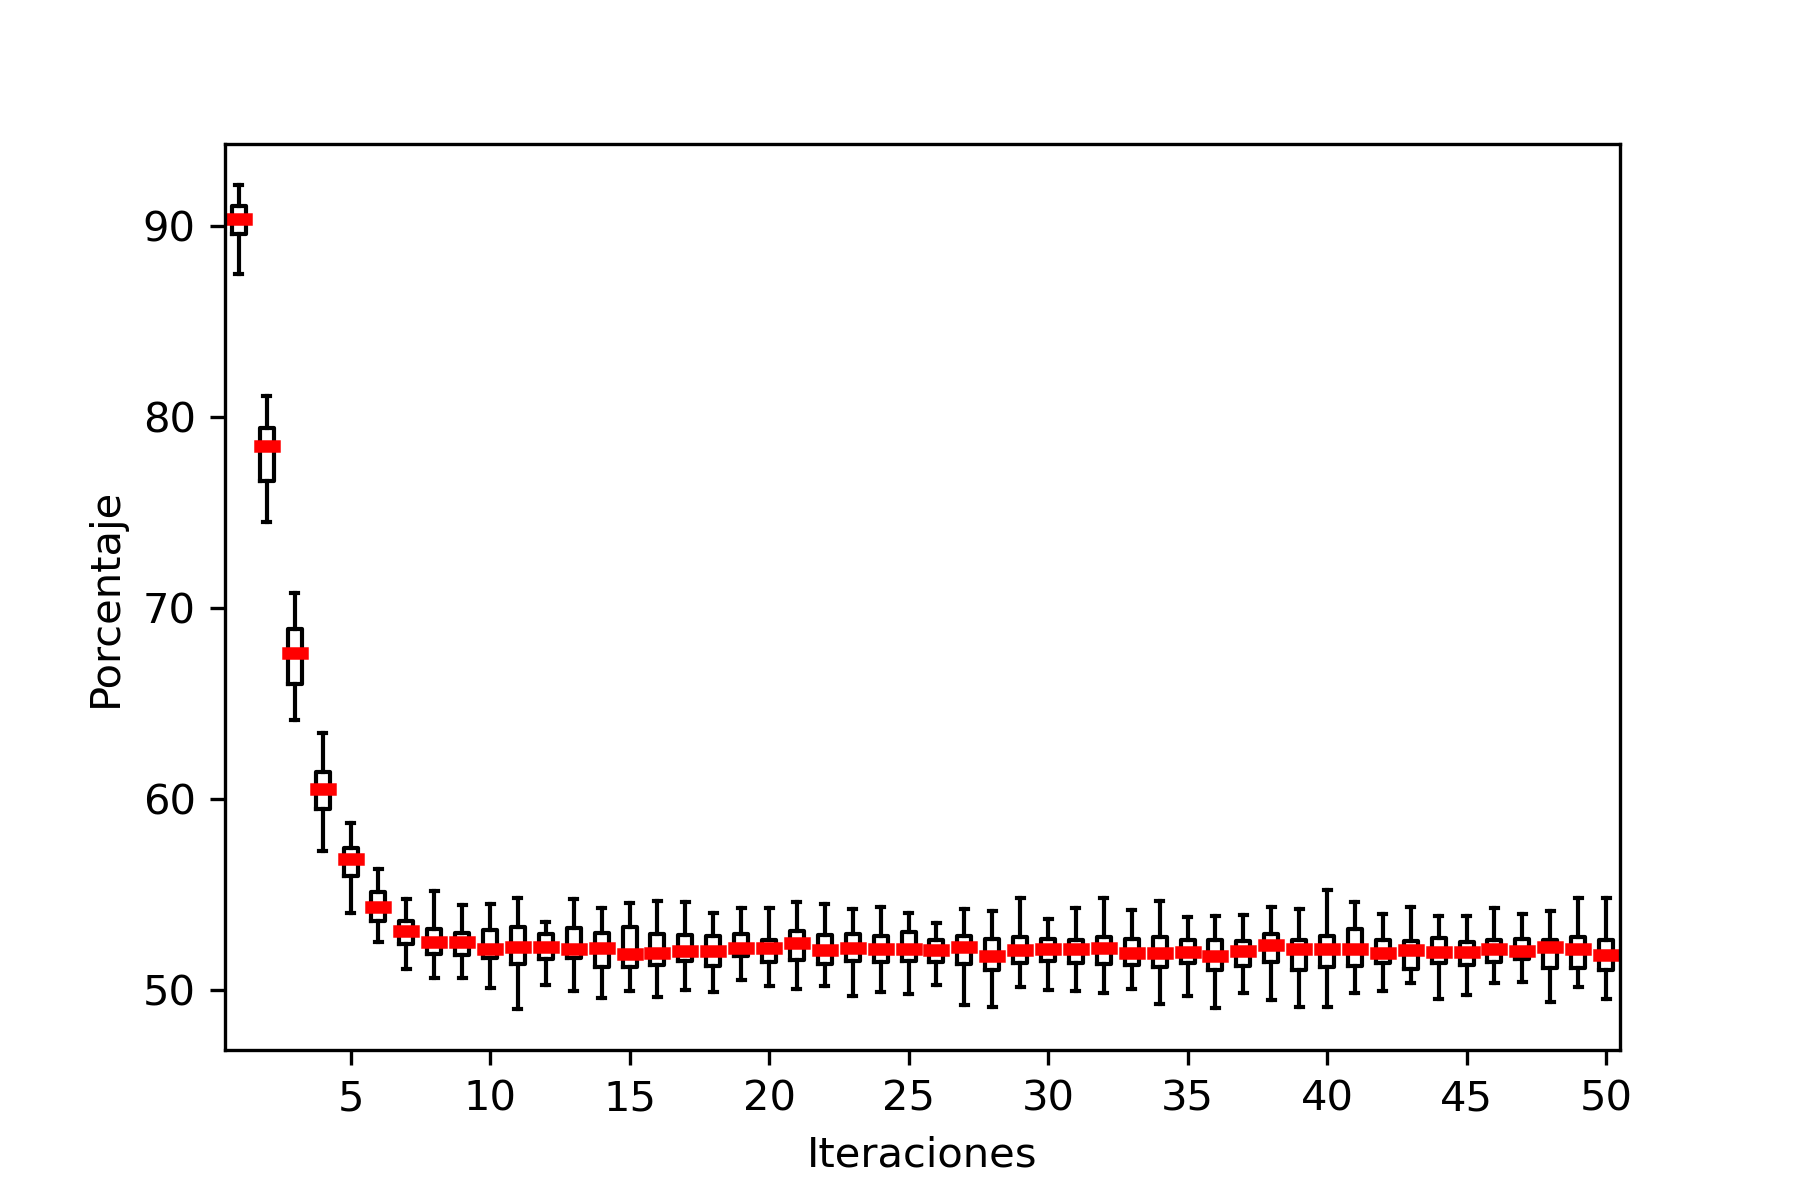
\includegraphics[width=\linewidth]{p8_v1_c1_n128000.png}
\caption{128000 partículas en c1.}
\end{subfigure}
\begin{subfigure}[b]{0.40\linewidth}
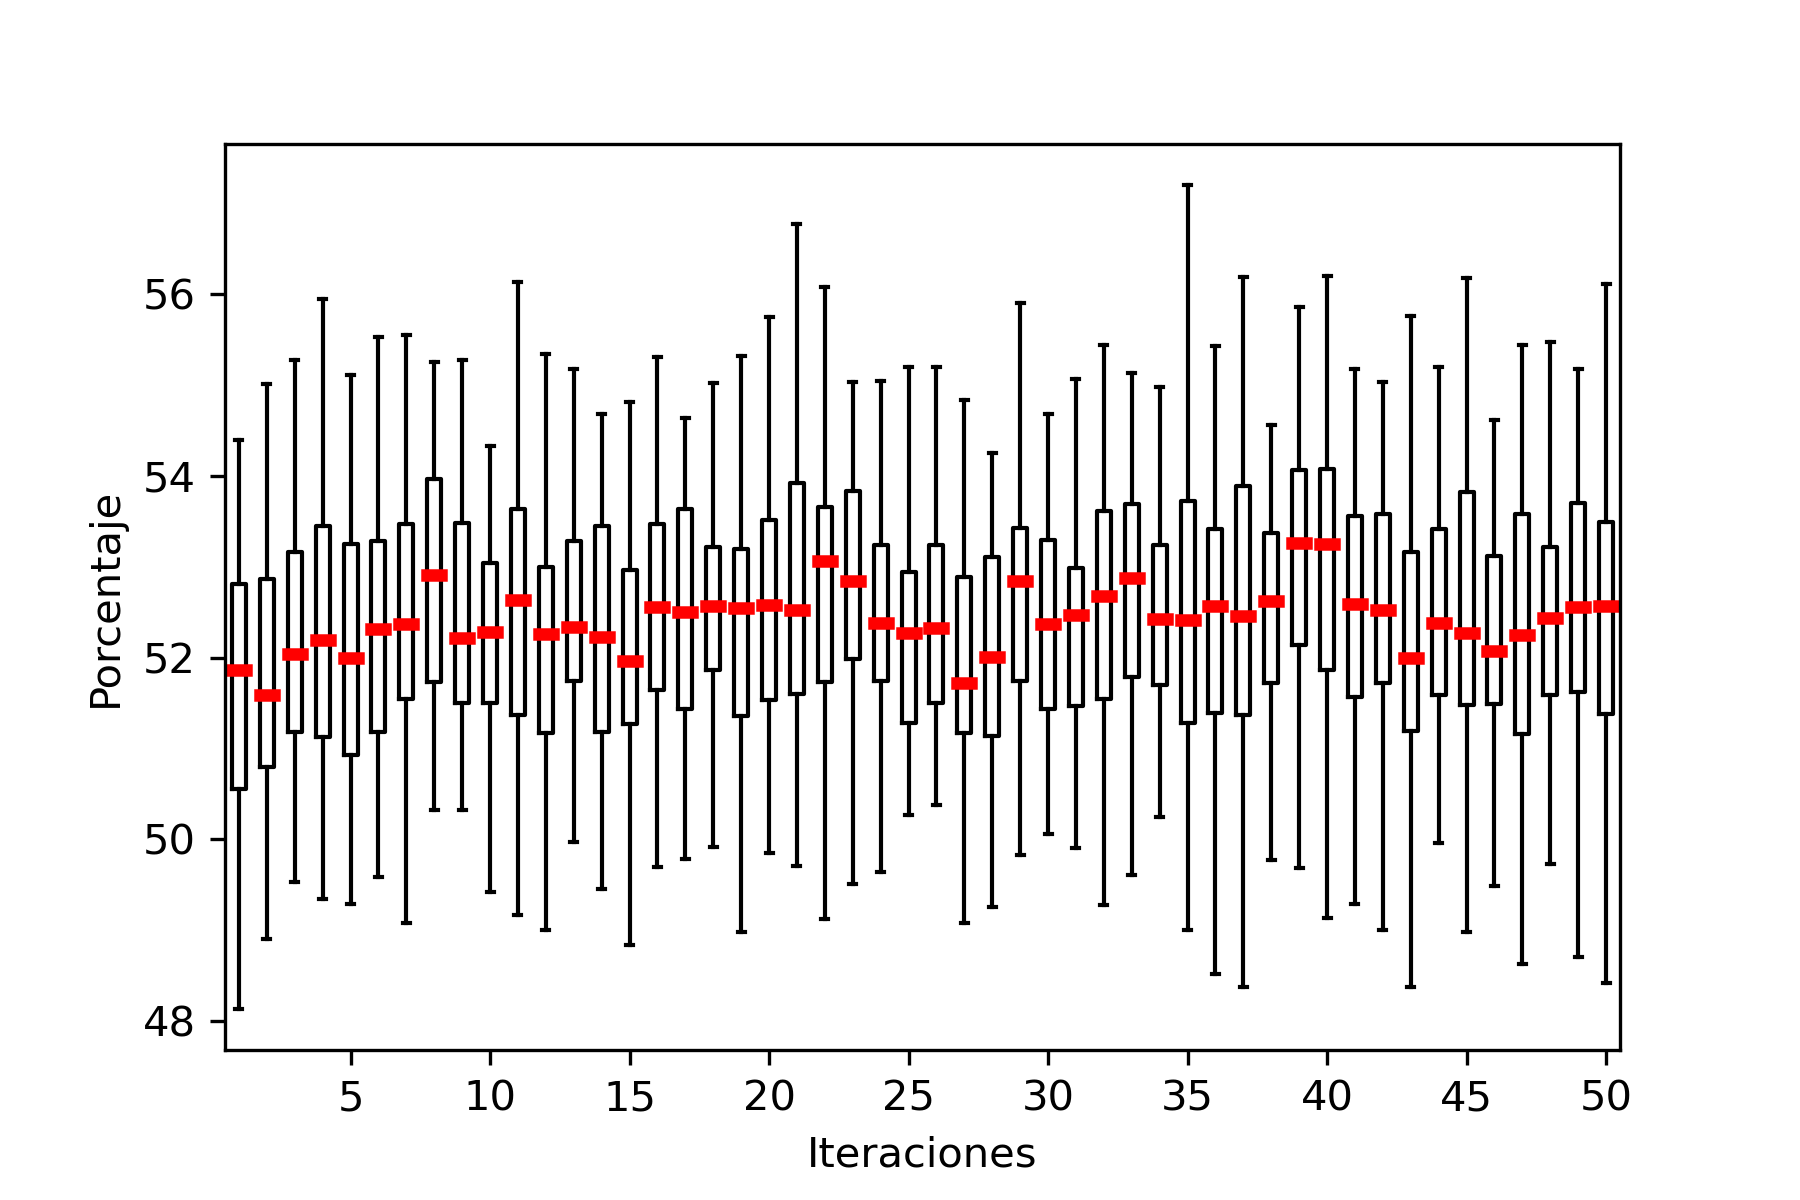
\includegraphics[width=\linewidth]{p8_v1_c2_n128000.png}
\caption{128000 partículas en c2.}
\end{subfigure}
\caption{Gráficas de porcentaje en diferentes puntos críticos.}
\label{fig:westminster}
\end{figure}

\begin{figure}[H]
\centering
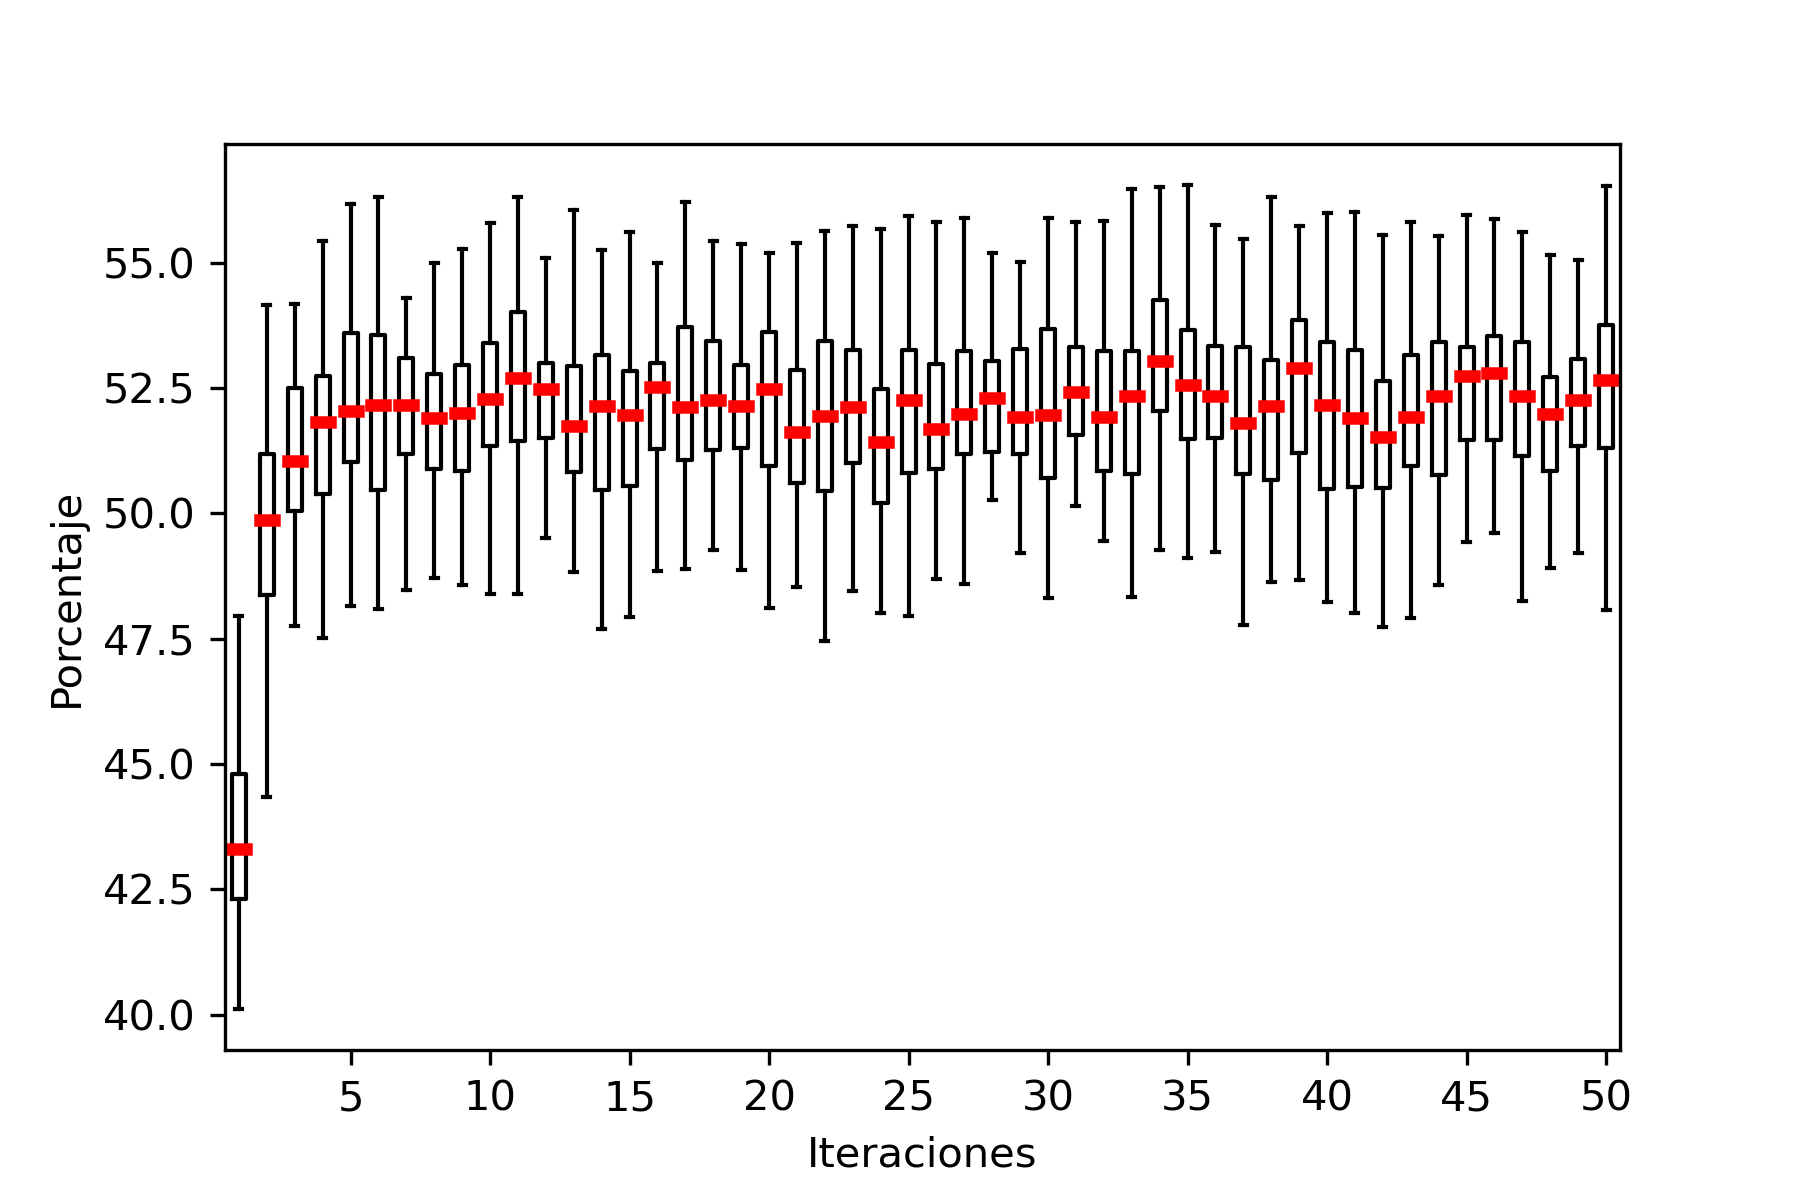
\includegraphics[width=80mm]{p8_v1_c3_n128000.png}
\caption{\label{fig3} 128000 partículas en c3.}
\end{figure}

\begin{table}[h!]
\centering
\caption{Prueba estadística Anova.}
 \begin{tabular}{||r r r||} 
 \hline
 Partículas & F & P  \\ [0.5ex] 
 \hline\hline
 16000 & 255.8 & 3.3 \\
 \hline
 32000 & 133.7 & 8.1\\ 
 \hline
 64000 & 116.7 & 1.16  \\
 \hline
 128000 & 170.5 & 3.8 \\
 \hline
\end{tabular}
\label{table:1}
\end{table}

\begin{figure}[H]
\centering
\begin{subfigure}[b]{0.40\linewidth}
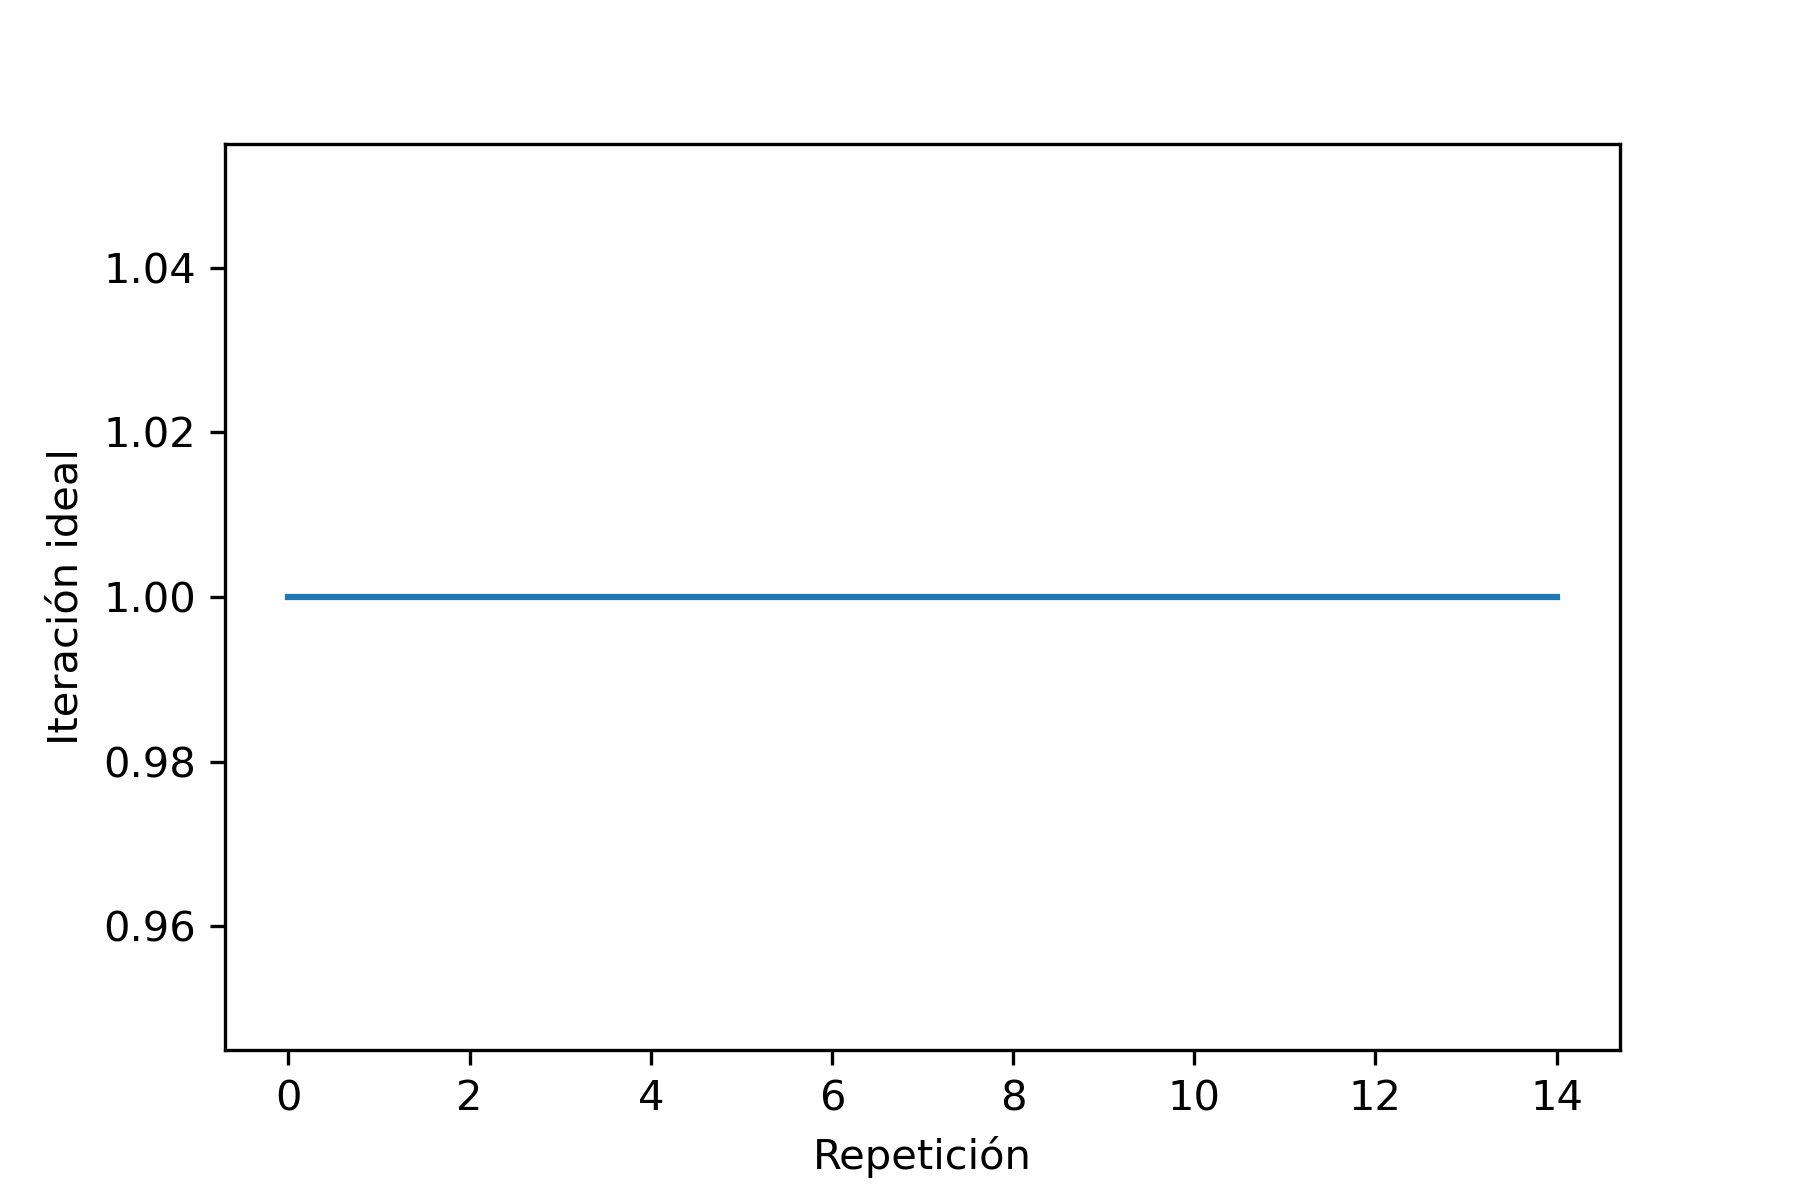
\includegraphics[width=\linewidth]{p8_v2_r1_c0_v0.png}
\caption{16000 partículas en c1.}
\end{subfigure}
\begin{subfigure}[b]{0.40\linewidth}
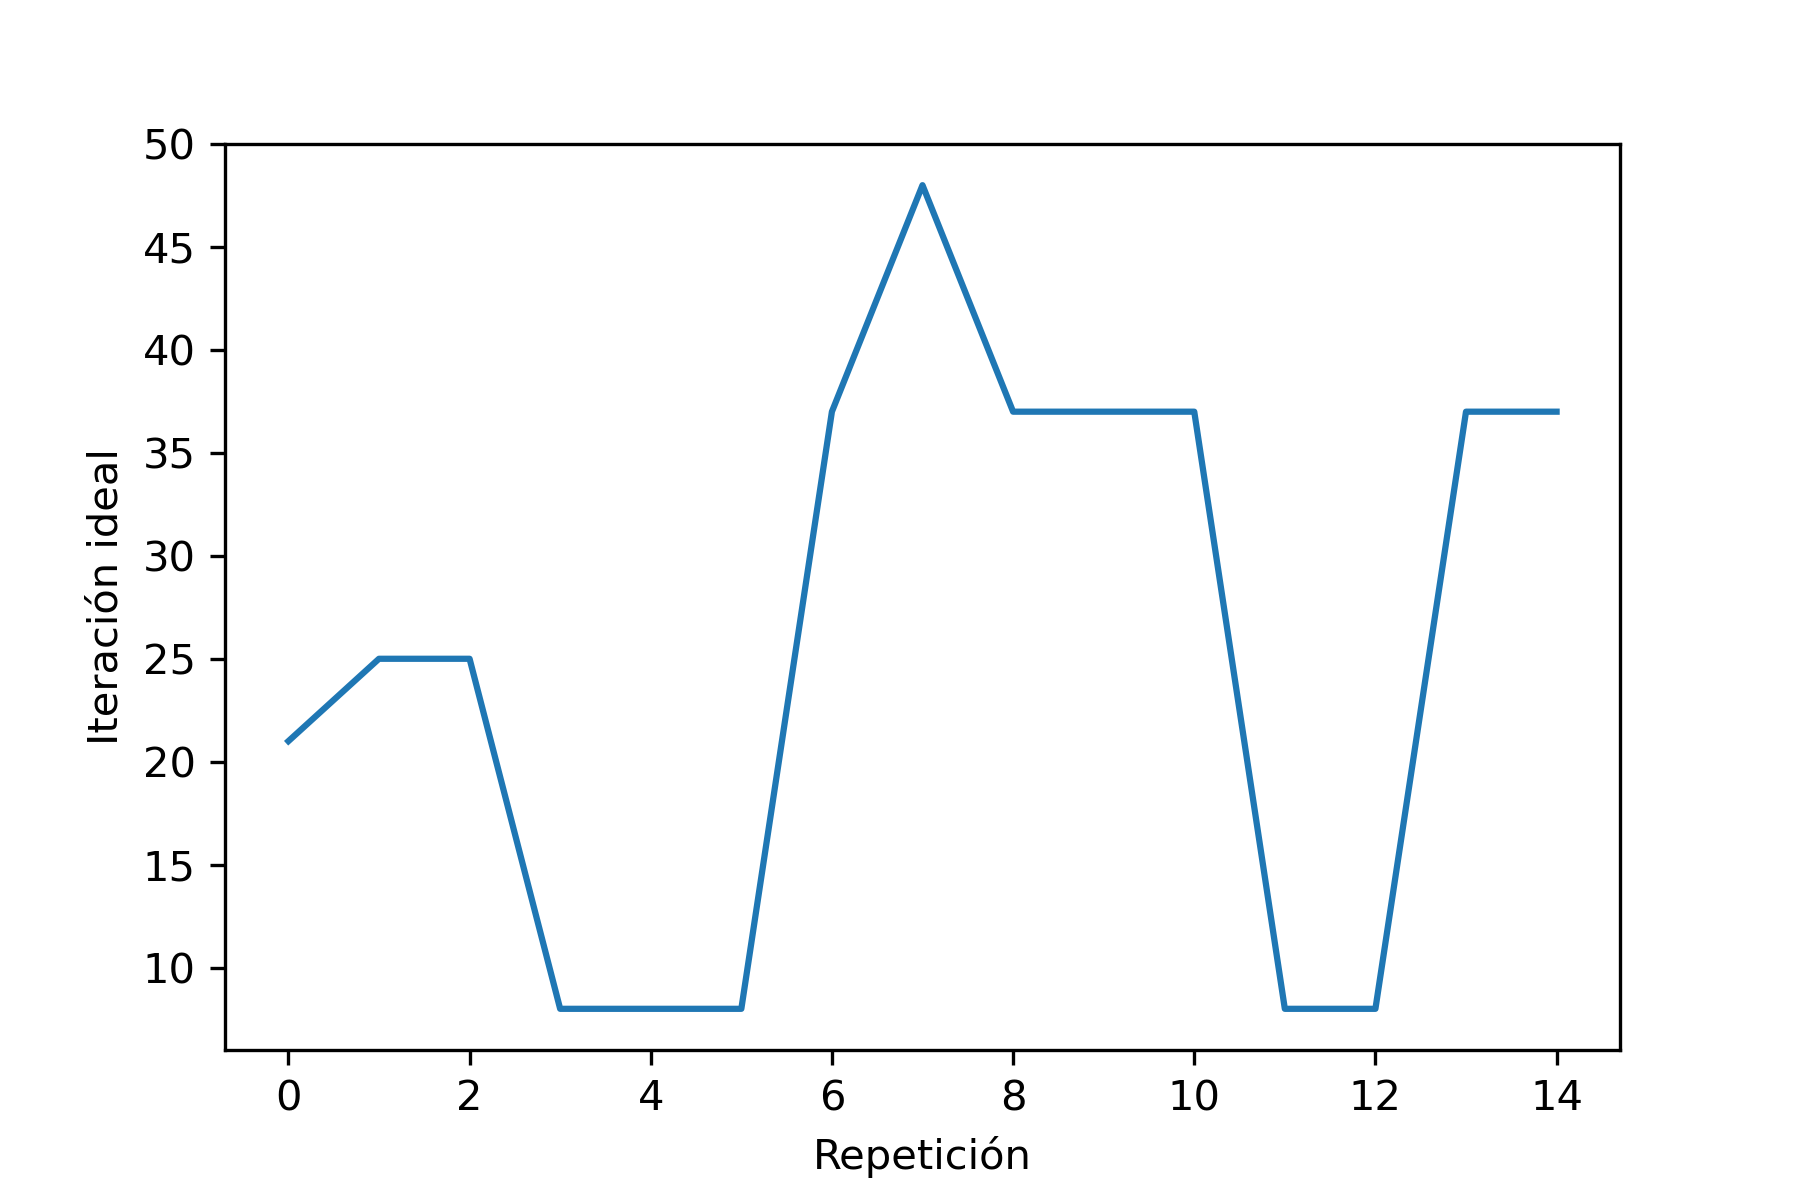
\includegraphics[width=\linewidth]{p8_v2_r1_c1_v0.png}
\caption{16000 partículas en c2.}
\end{subfigure}
\caption{Gráfica de iteración ideal por repetición en diferentes puntos críticos.}
\label{fig:westminster}
\end{figure}

\begin{figure}[H]
\centering
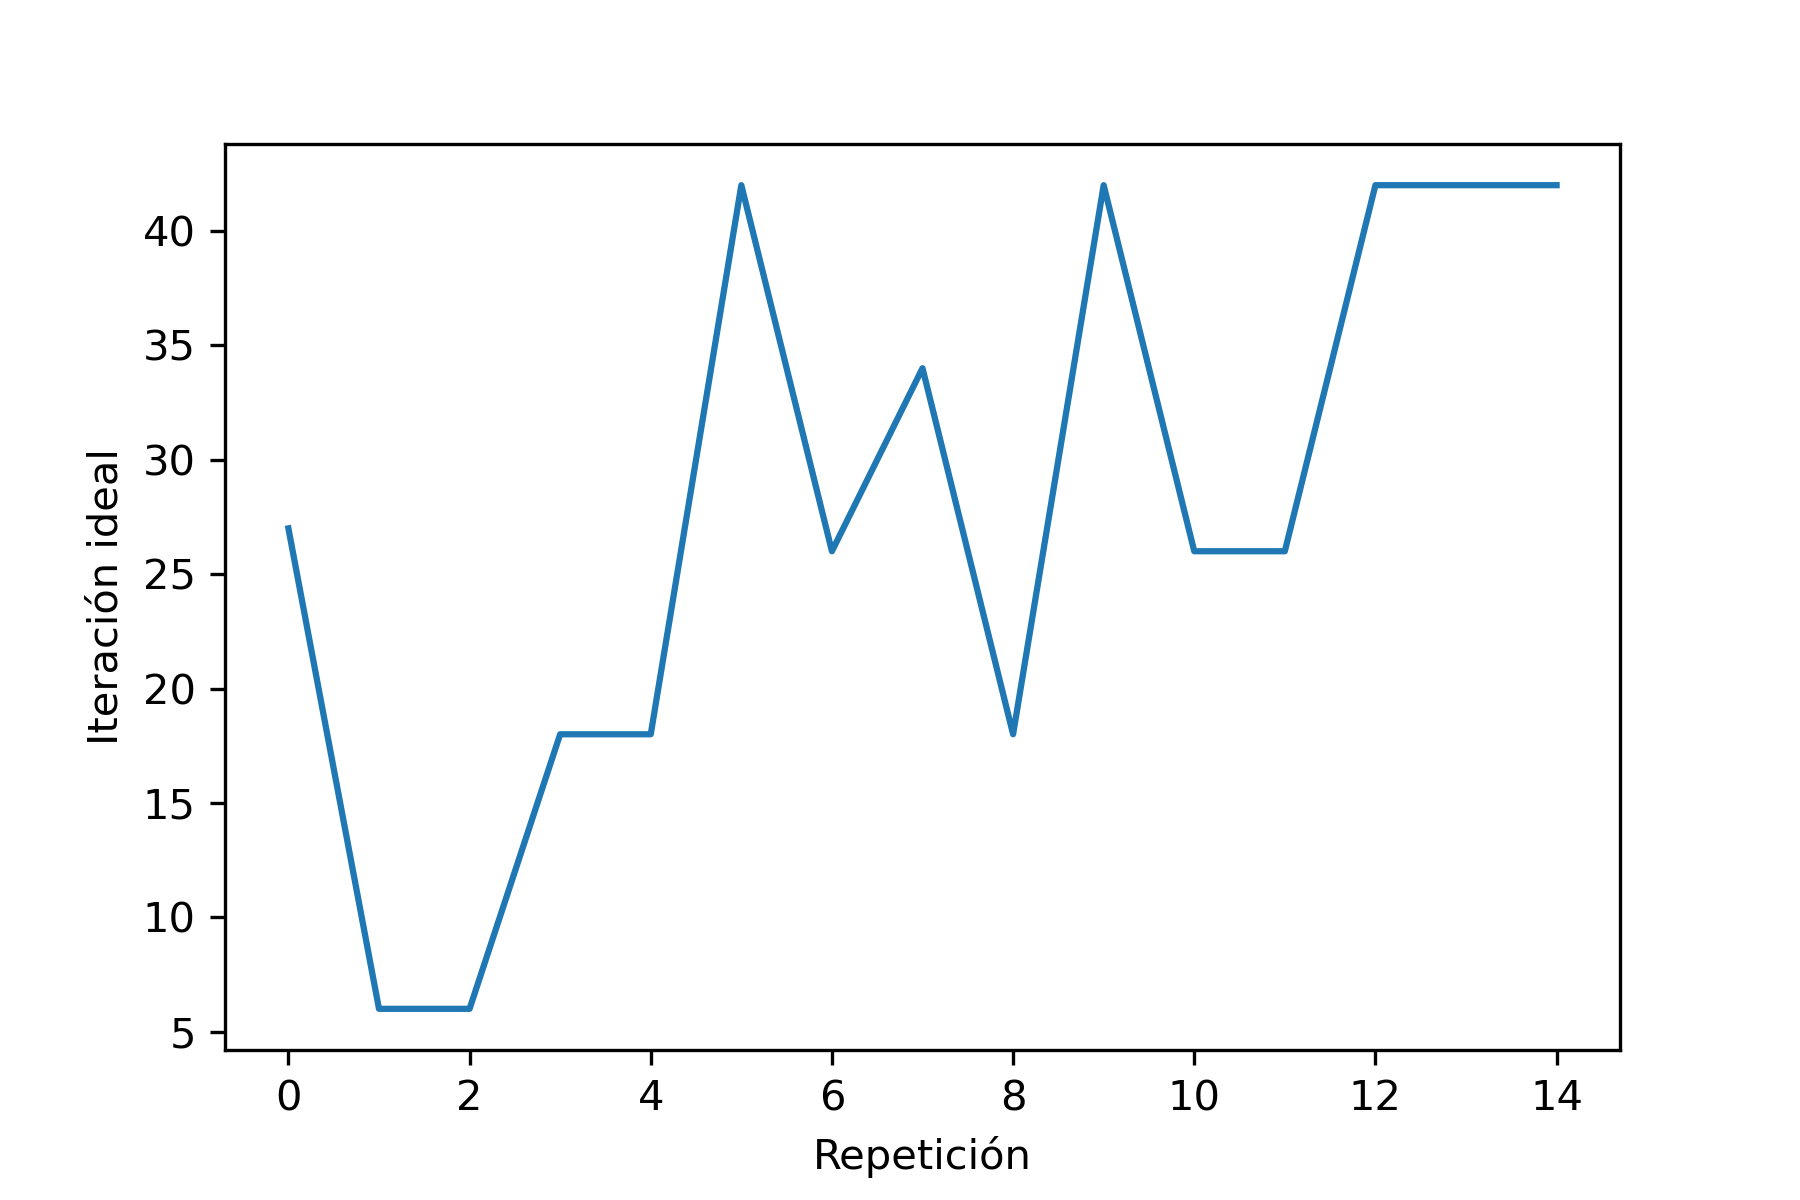
\includegraphics[width=80mm]{p8_v2_r1_c2_v0.png}
\caption{\label{fig3}Gráfica de iteración ideal por repetición en 16000 partículas en c3.}
\end{figure}

\begin{figure}[H]
\centering
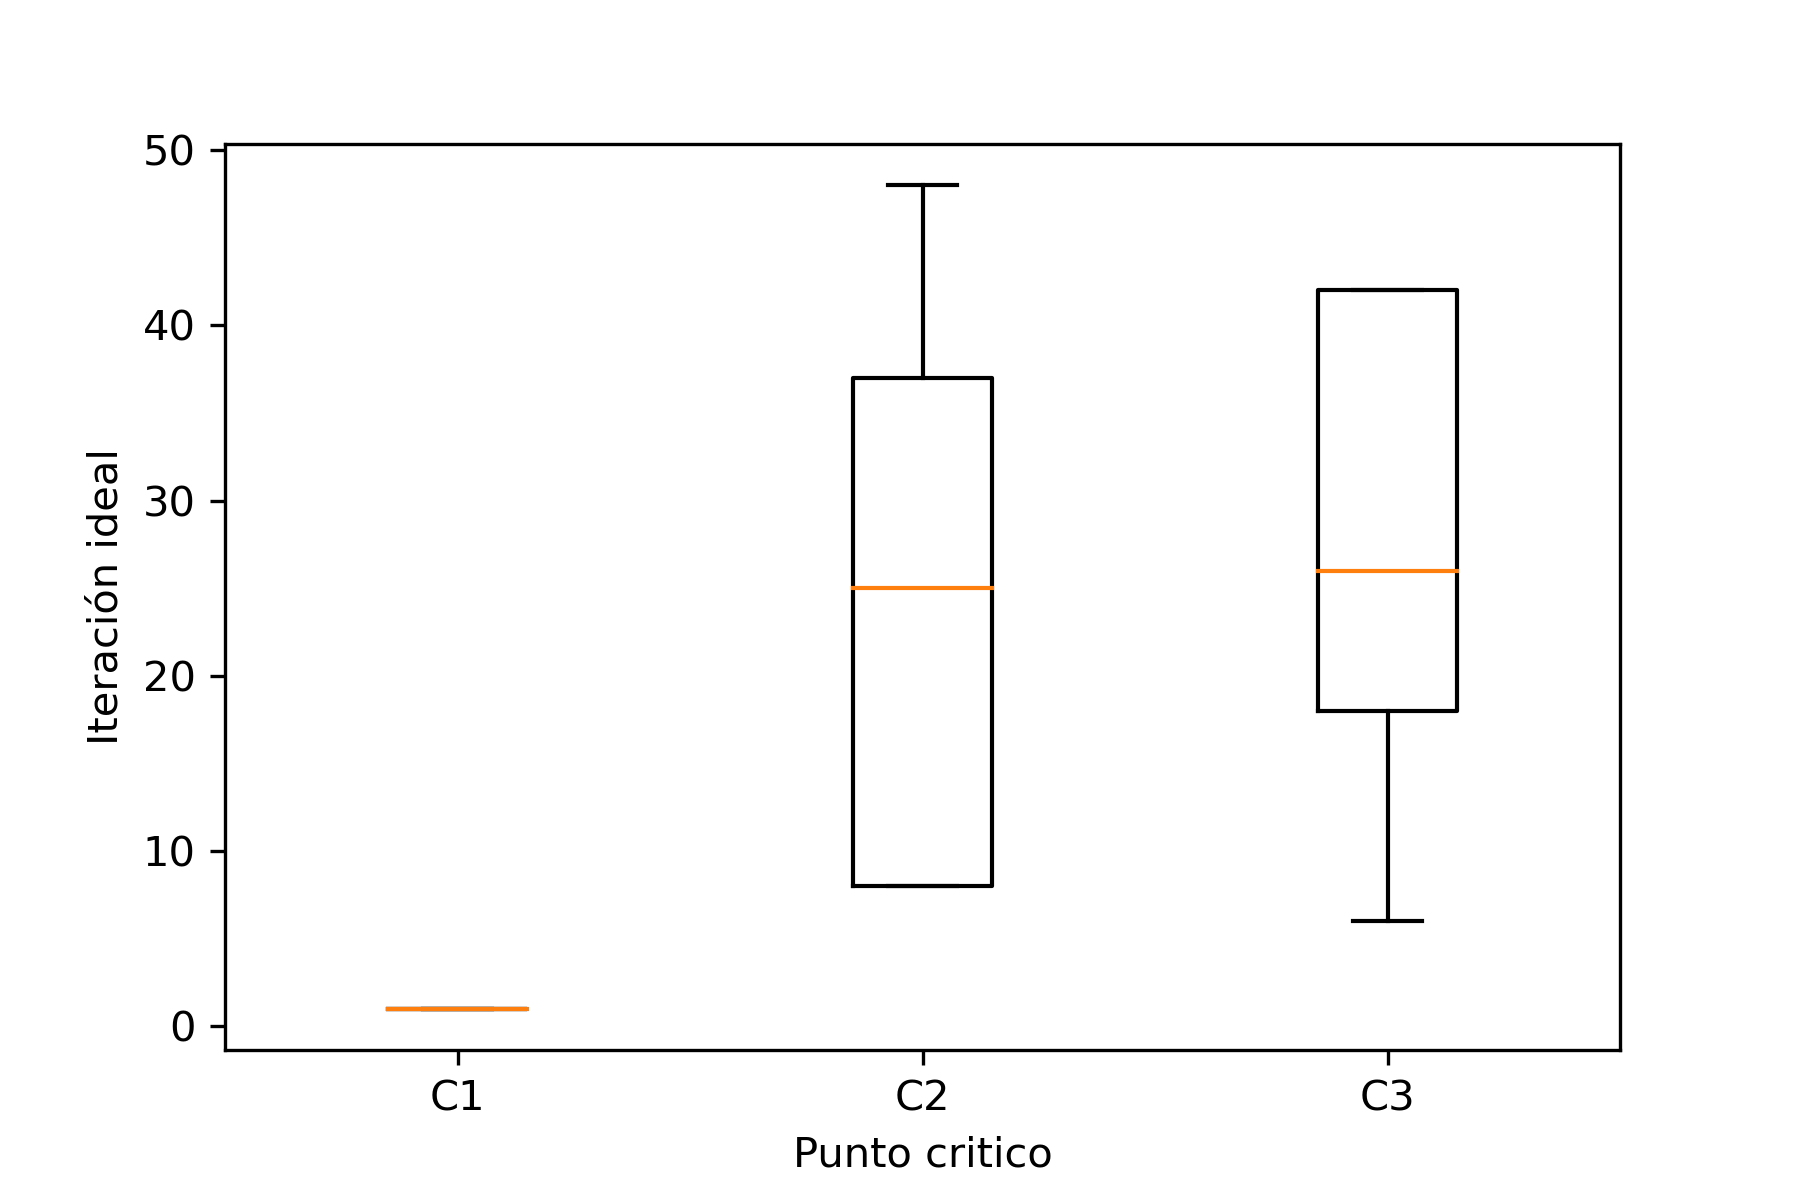
\includegraphics[width=80mm]{p8_v2_r1_c0_n0.png}
\caption{\label{fig3} Gráfica caja bigote de iteración ideal con diferentes puntos críticos.}
\end{figure}

\begin{figure}[H]
\centering
\begin{subfigure}[b]{0.40\linewidth}
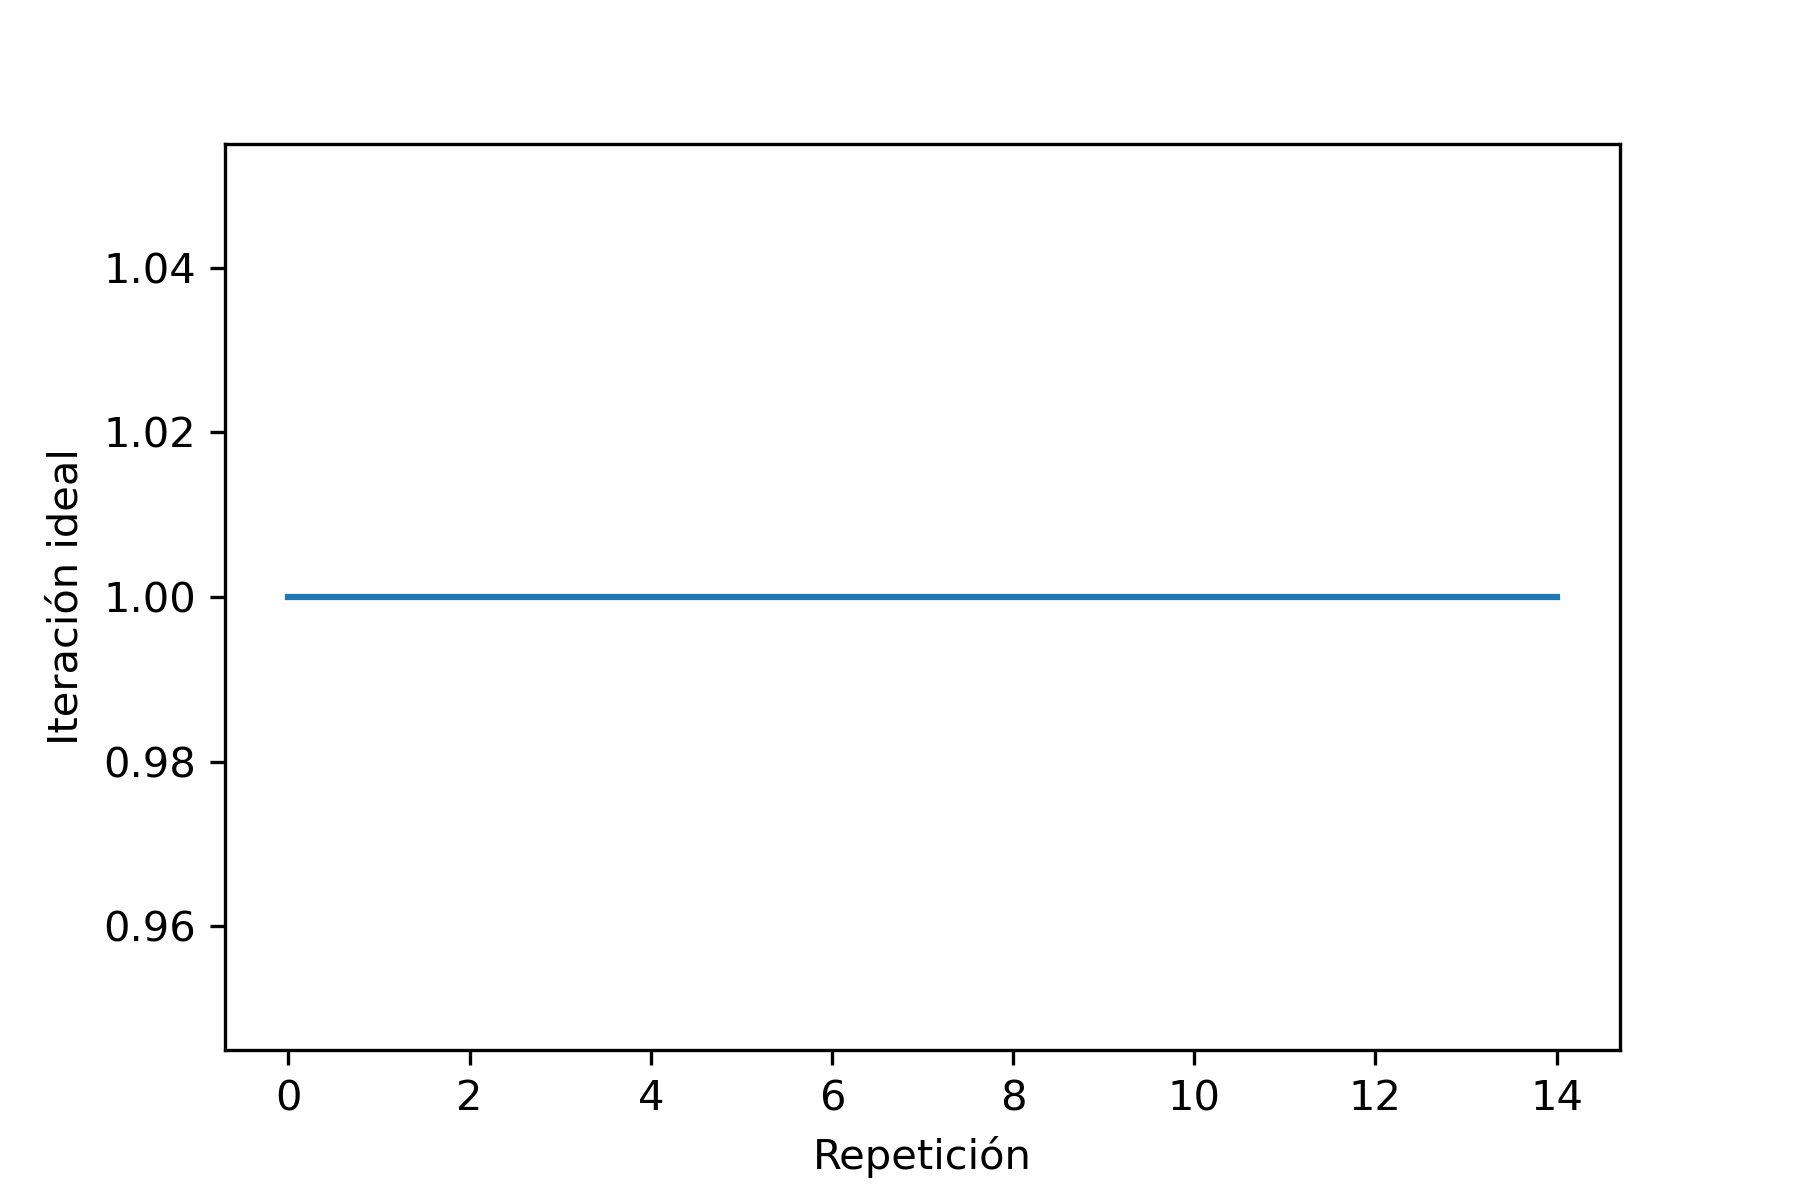
\includegraphics[width=\linewidth]{p8_v2_r1_c0_v1.png}
\caption{32000 partículas en c1.}
\end{subfigure}
\begin{subfigure}[b]{0.40\linewidth}
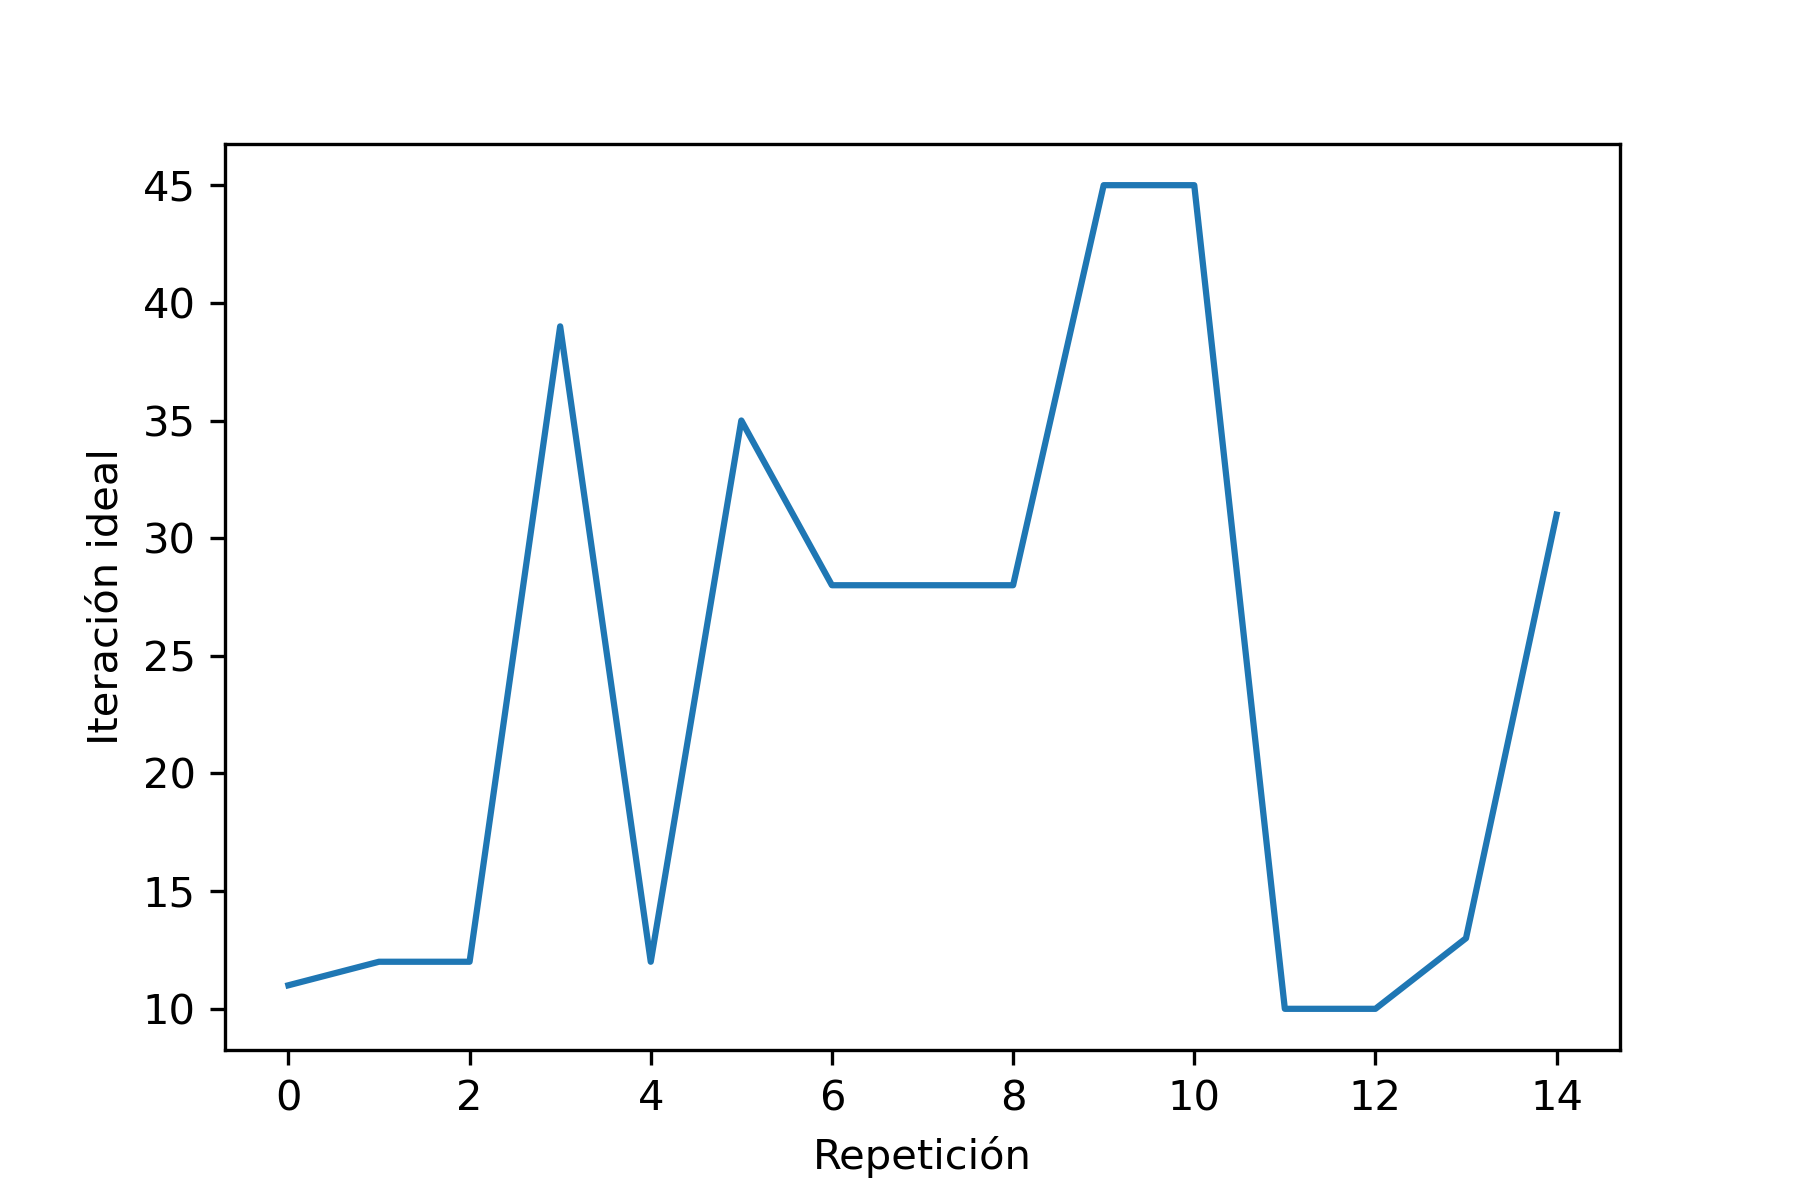
\includegraphics[width=\linewidth]{p8_v2_r1_c1_v1.png}
\caption{32000 partículas en c2.}
\end{subfigure}
\caption{Gráfica de iteración ideal por repetición en diferentes puntos críticos.}
\label{fig:westminster}
\end{figure}

\begin{figure}[H]
\centering
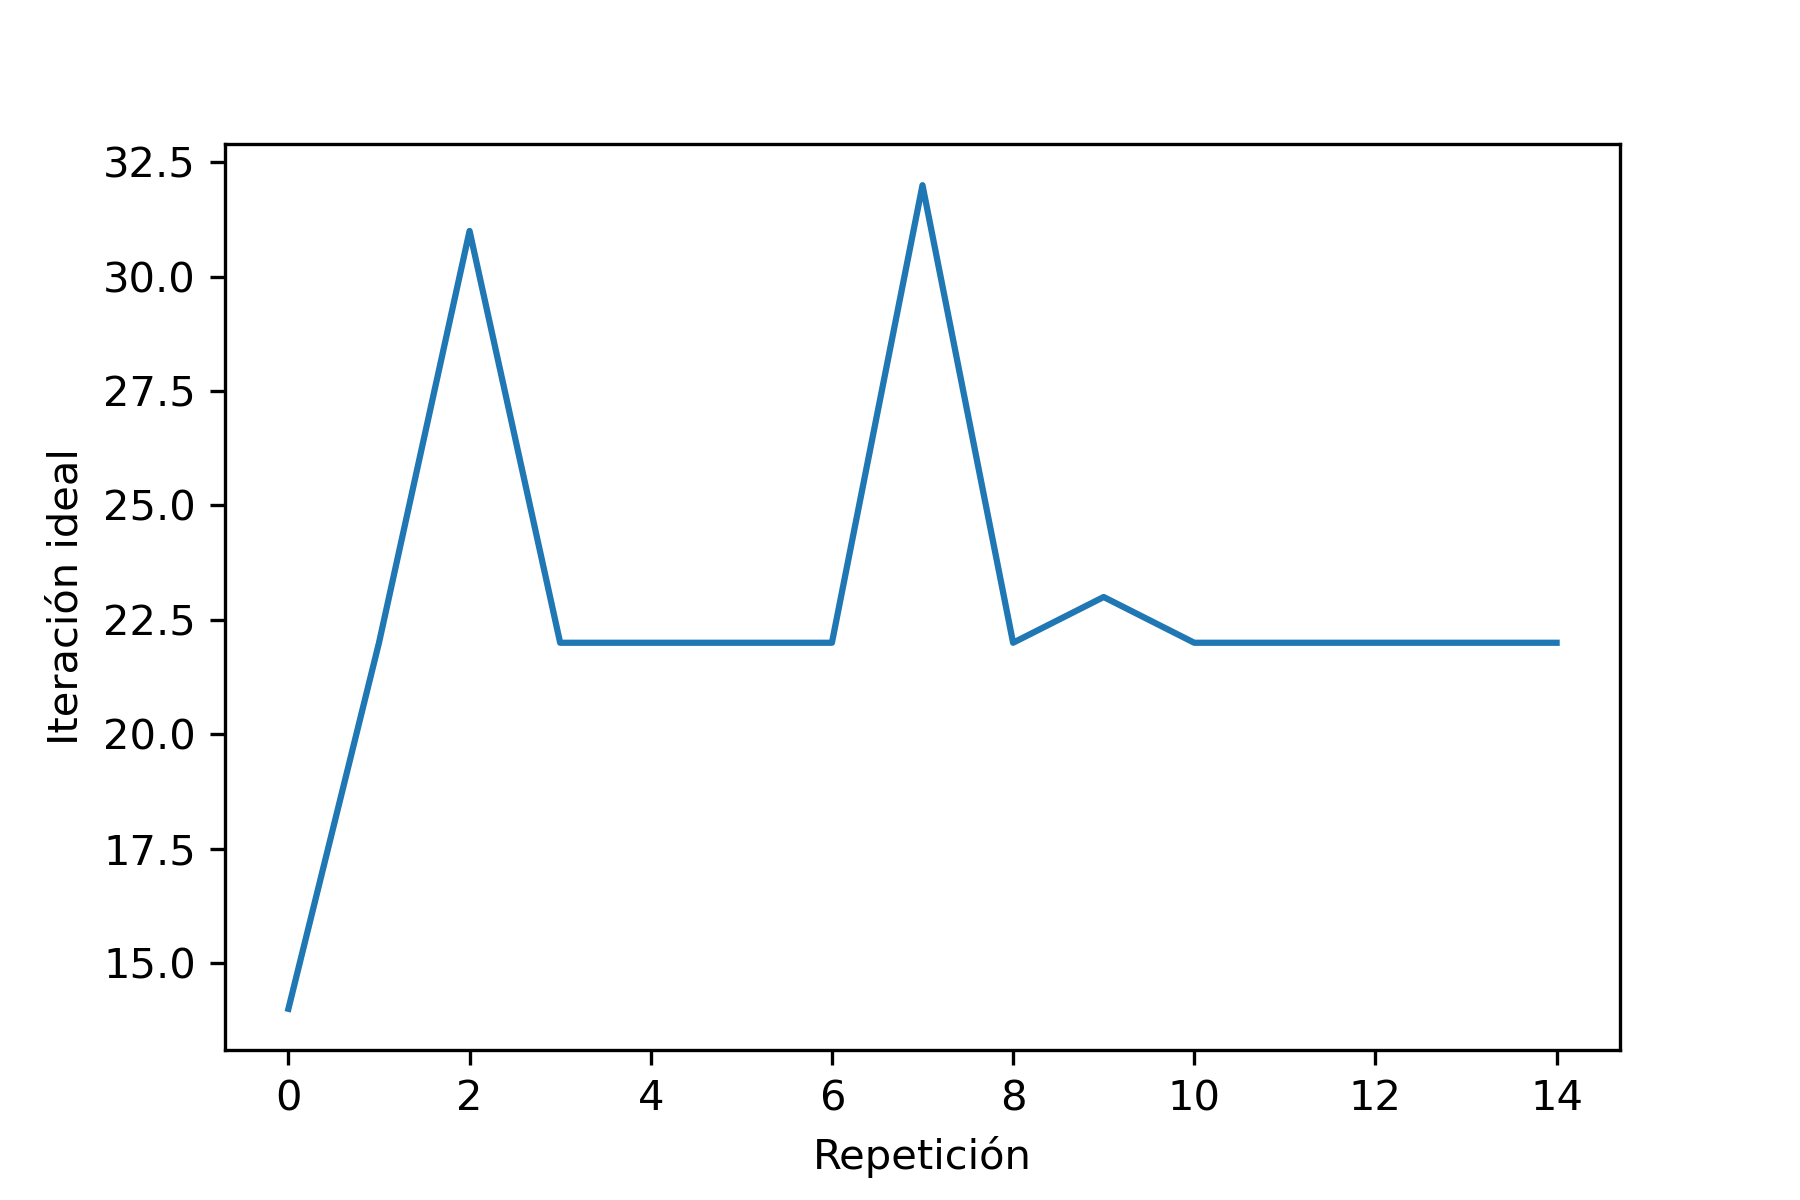
\includegraphics[width=80mm]{p8_v2_r1_c2_v1.png}
\caption{\label{fig3} Gráfica de iteración ideal por repetición en 32000 partículas en c3.}
\end{figure}

\begin{figure}[H]
\centering
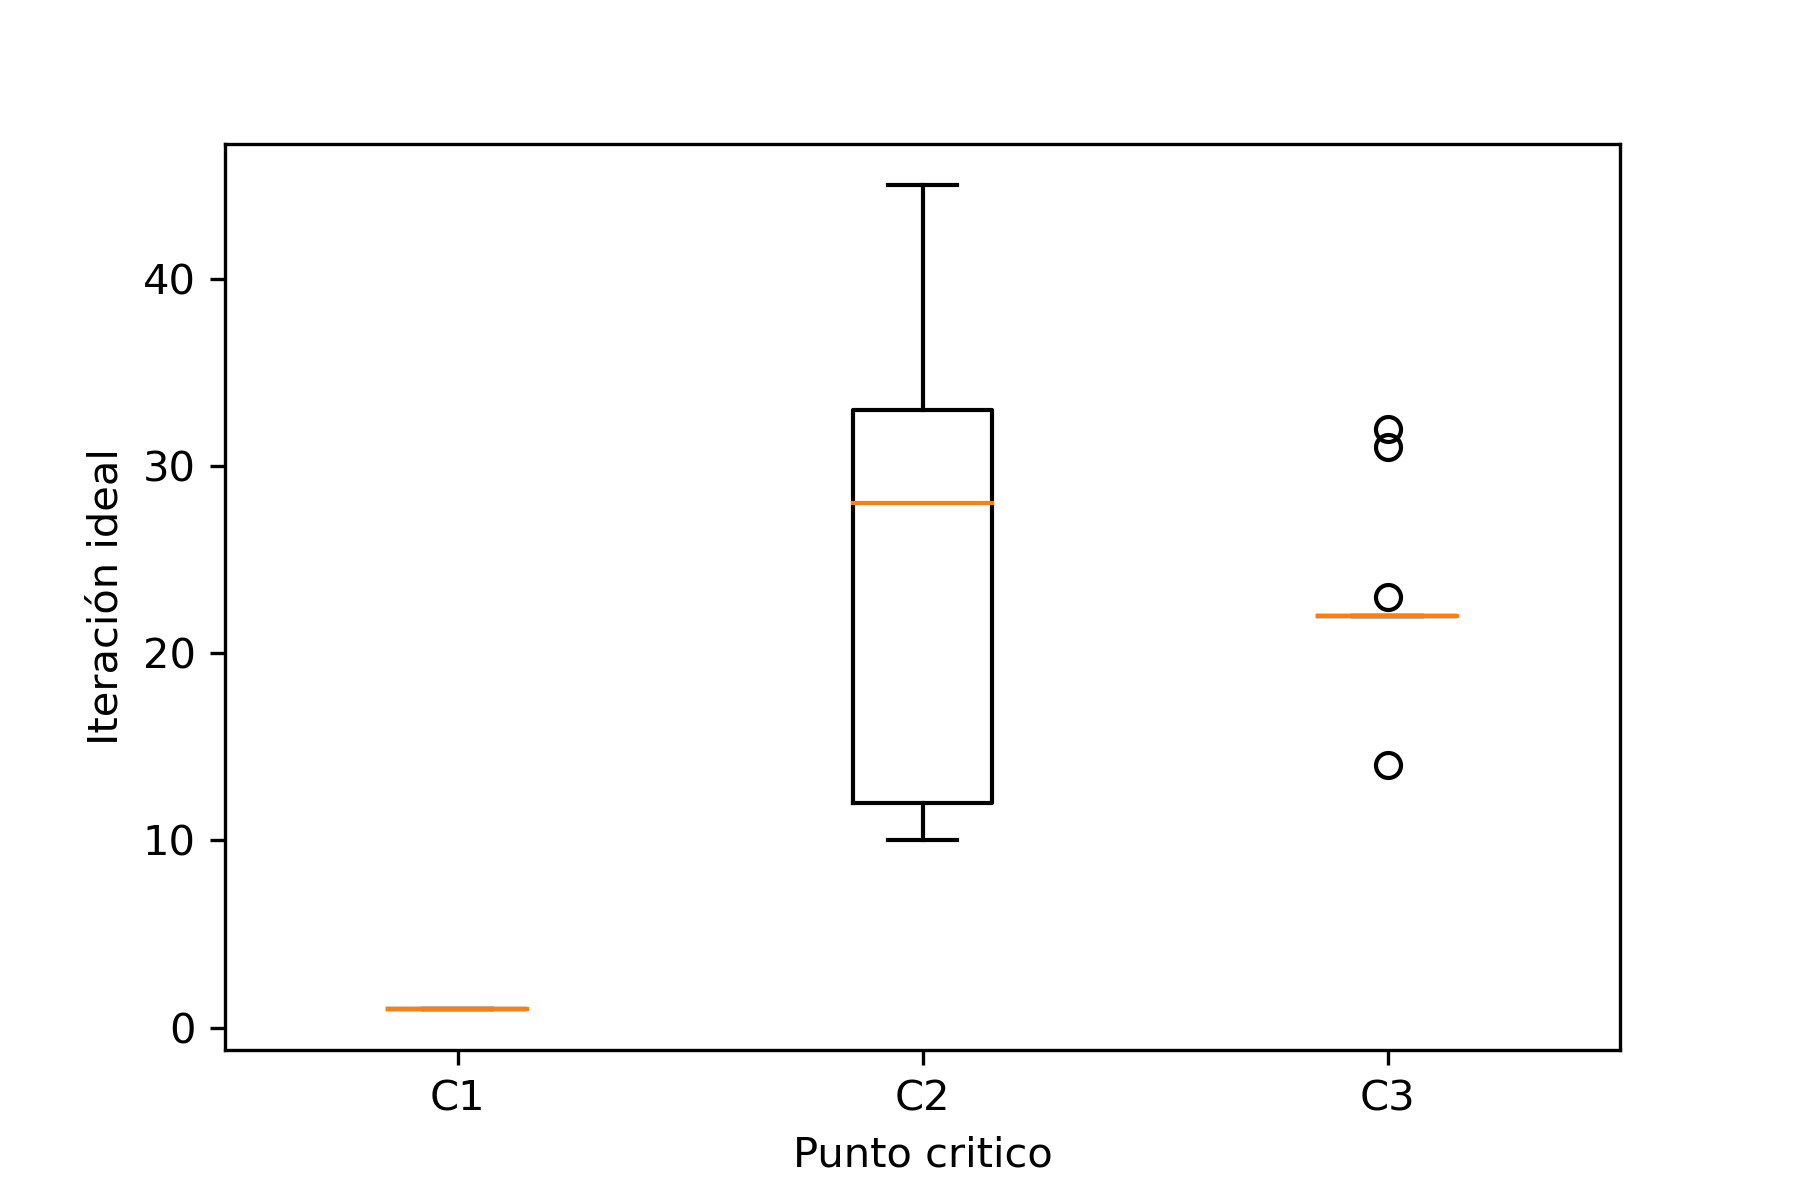
\includegraphics[width=80mm]{p8_v2_r1_c1_n1.png}
\caption{\label{fig3} Gráfica caja bigote de iteración ideal en diferentes puntos críticos.}
\end{figure}

\begin{figure}[H]
\centering
\begin{subfigure}[b]{0.40\linewidth}
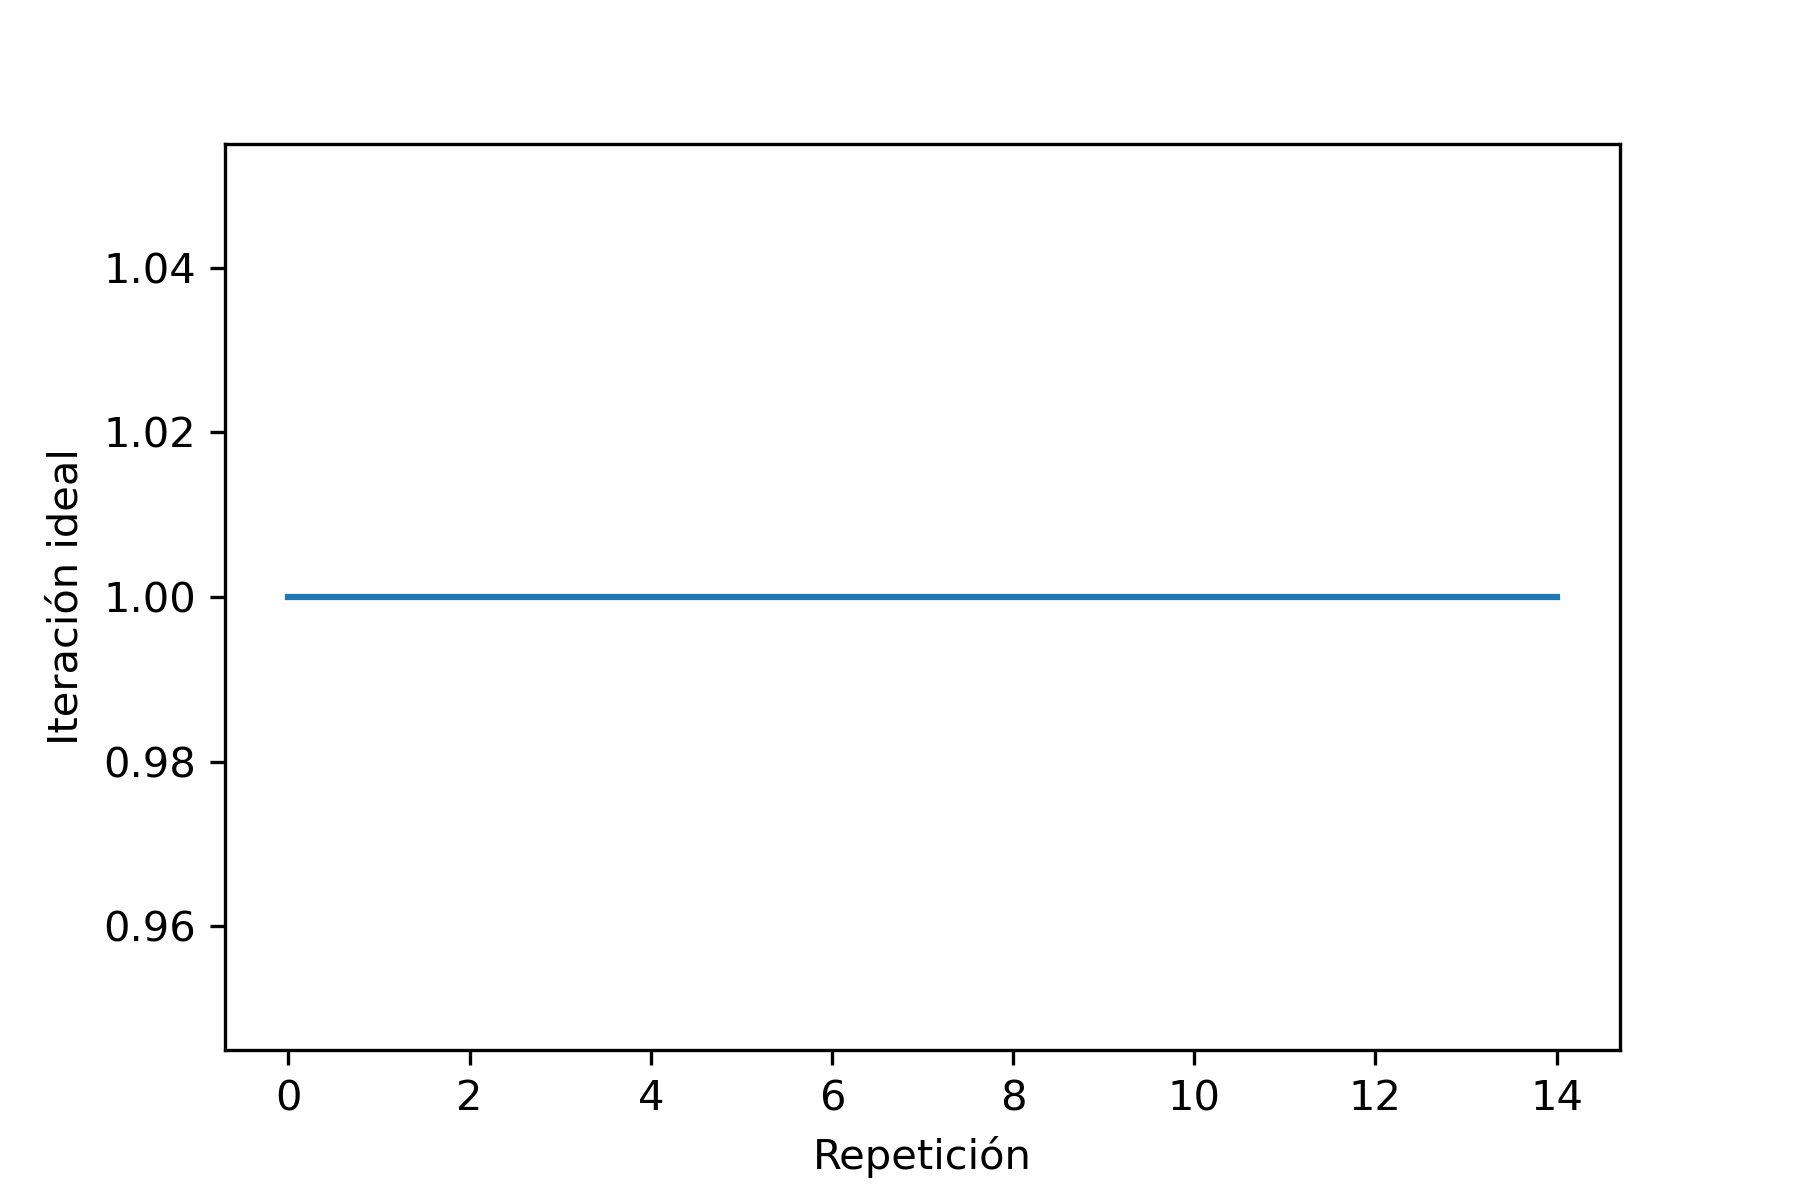
\includegraphics[width=\linewidth]{p8_v2_r1_c0_v2.png}
\caption{64000 partículas en c1.}
\end{subfigure}
\begin{subfigure}[b]{0.40\linewidth}
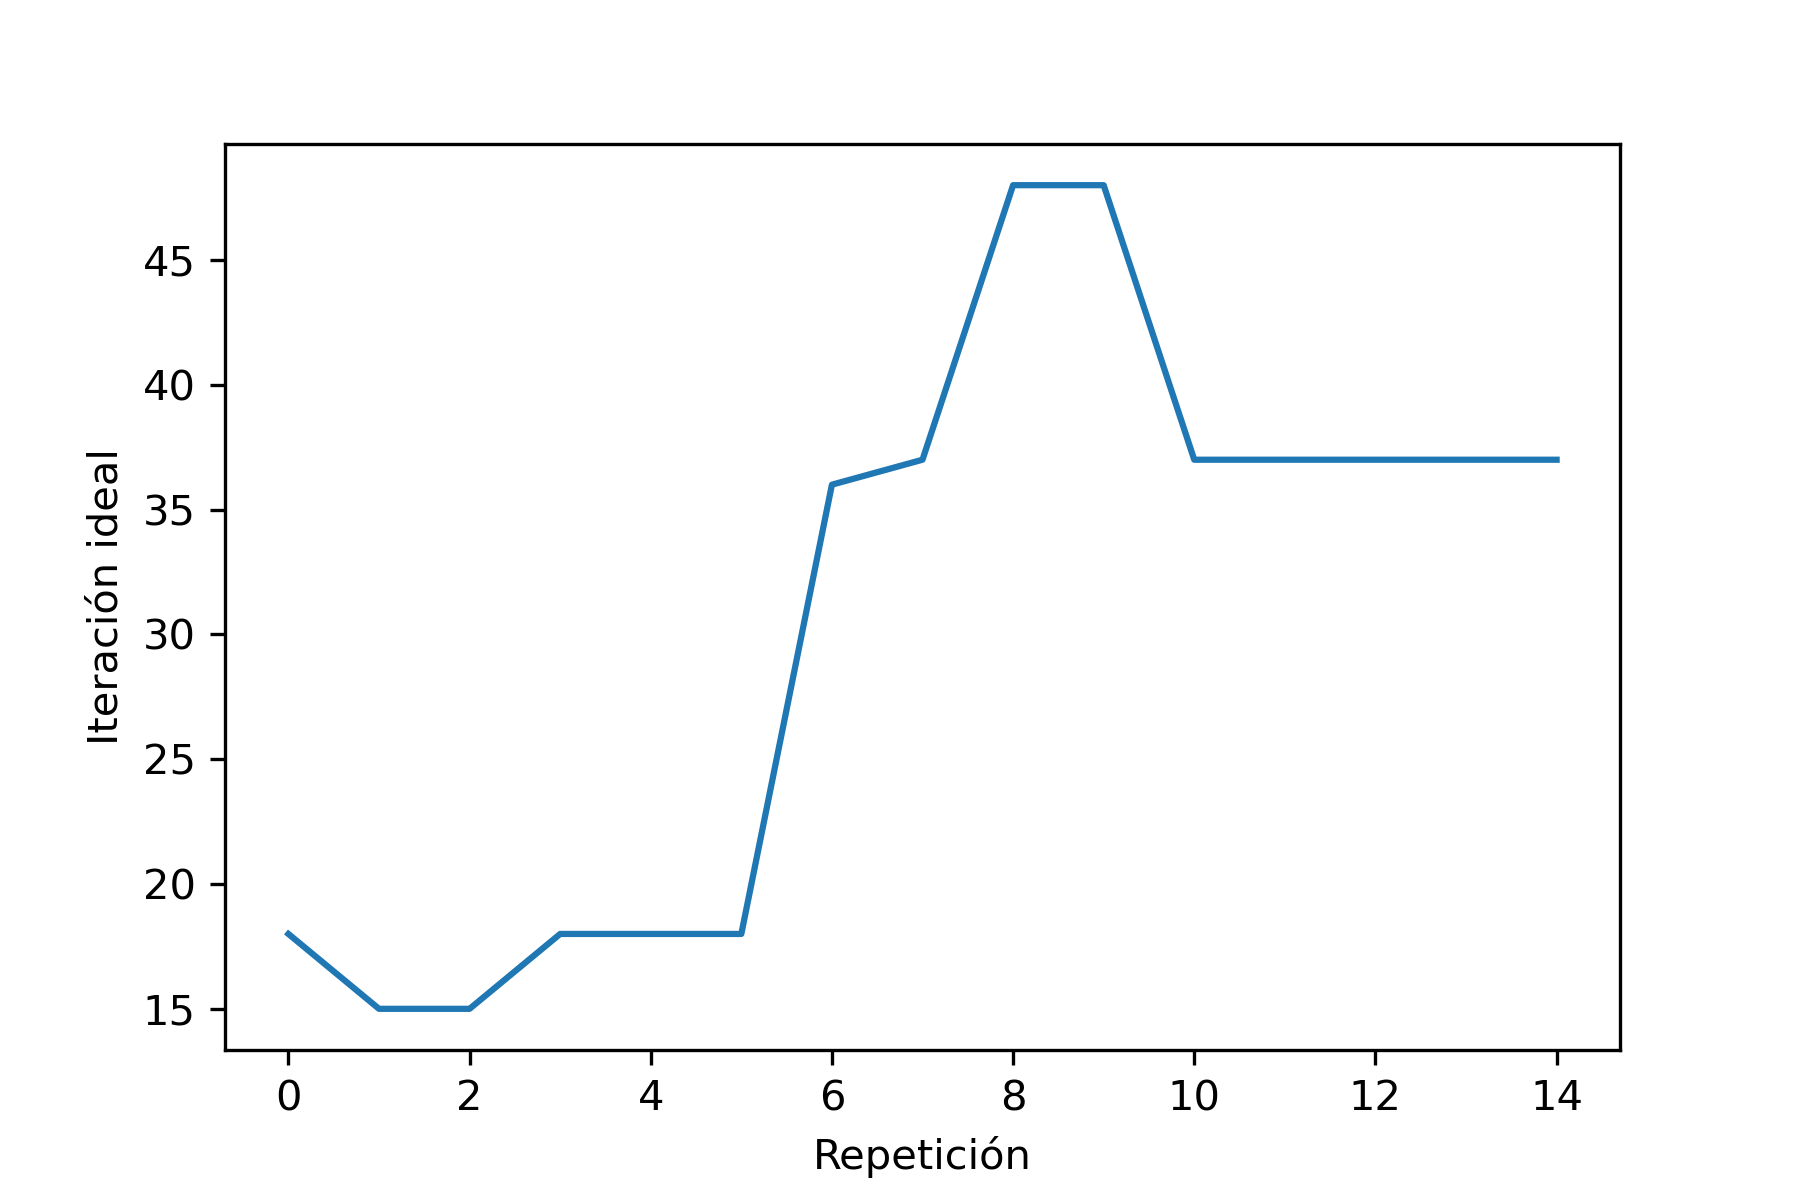
\includegraphics[width=\linewidth]{p8_v2_r1_c1_v2.png}
\caption{64000 partículas en c2.}
\end{subfigure}
\caption{Gráfica de iteración ideal por repetición en diferentes puntos críticos.}
\label{fig:westminster}
\end{figure}

\begin{figure}[H]
\centering
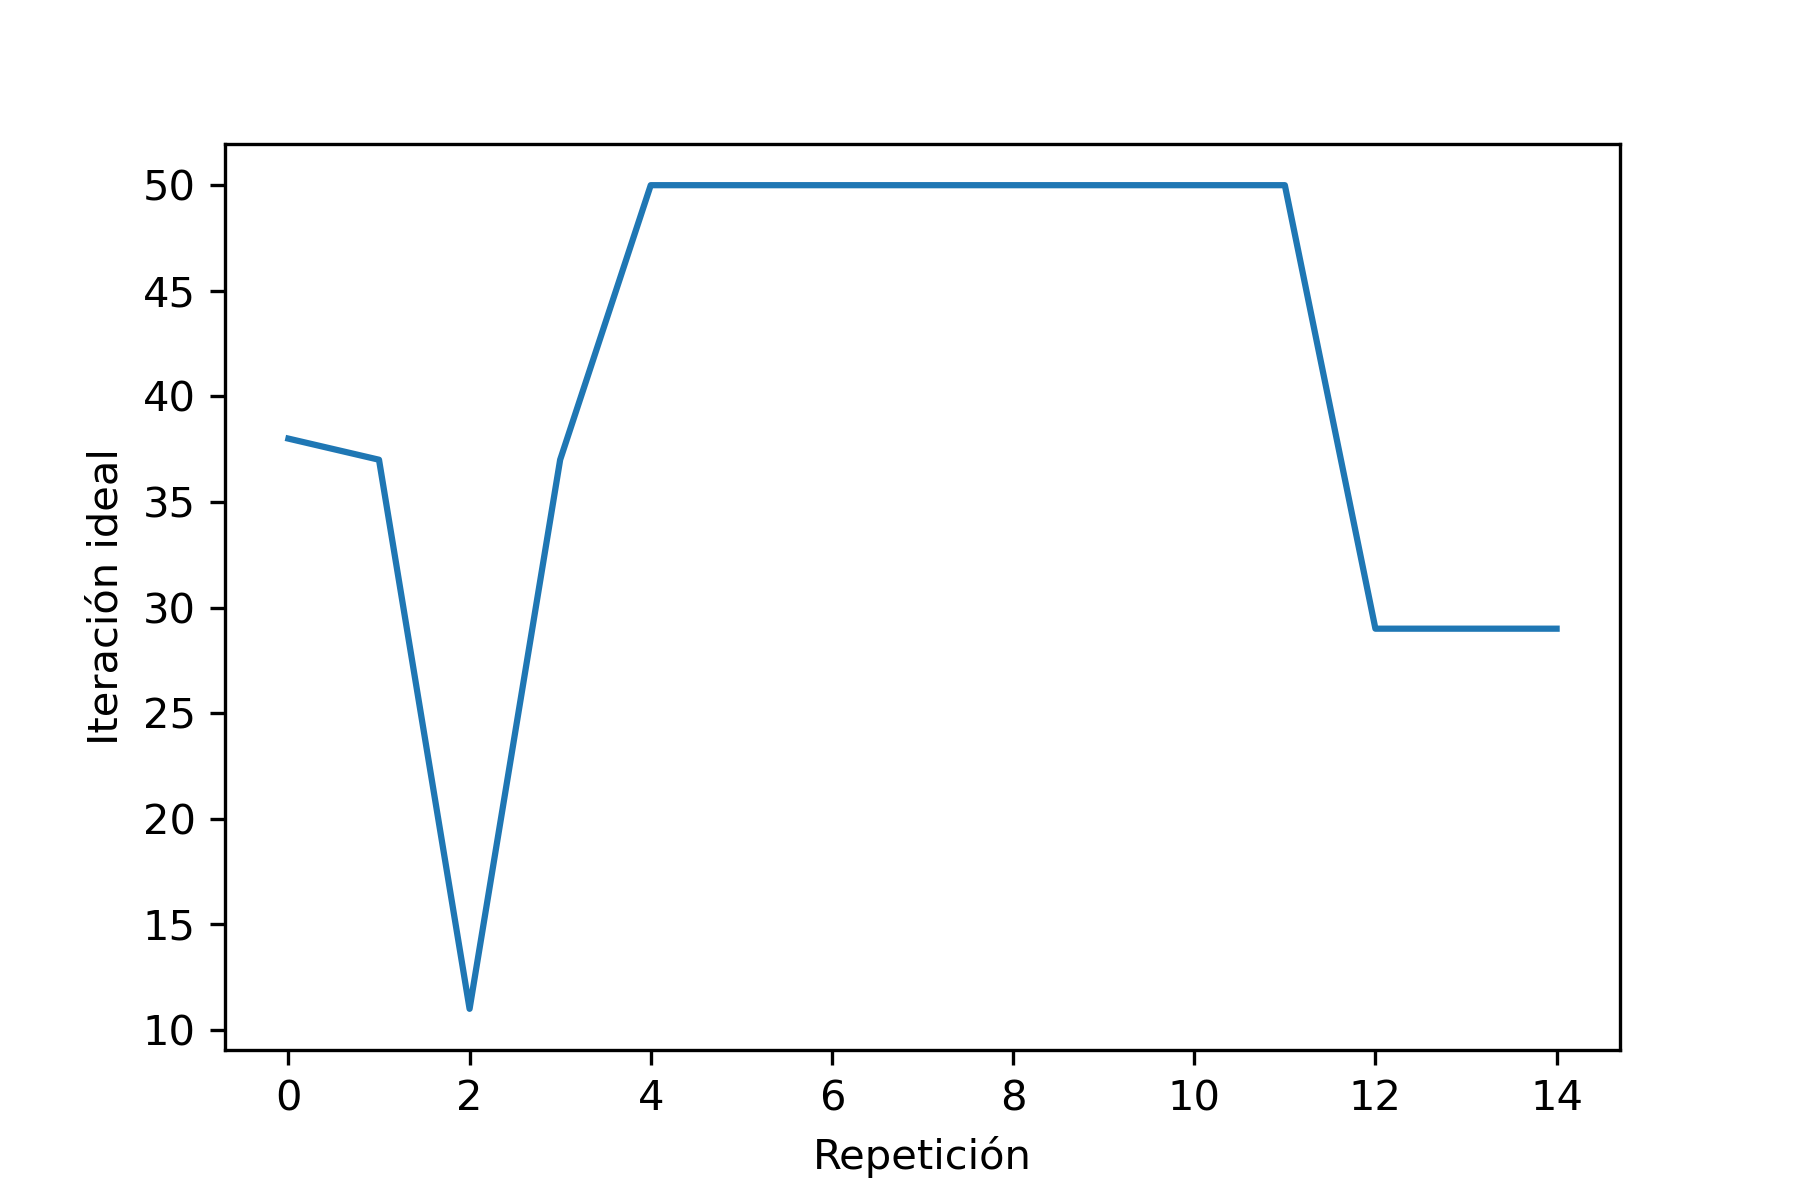
\includegraphics[width=80mm]{p8_v2_r1_c2_v2.png}
\caption{\label{fig3} Gráfica de iteración ideal por repetición 64000 partículas en c3.}
\end{figure}

\begin{figure}[H]
\centering
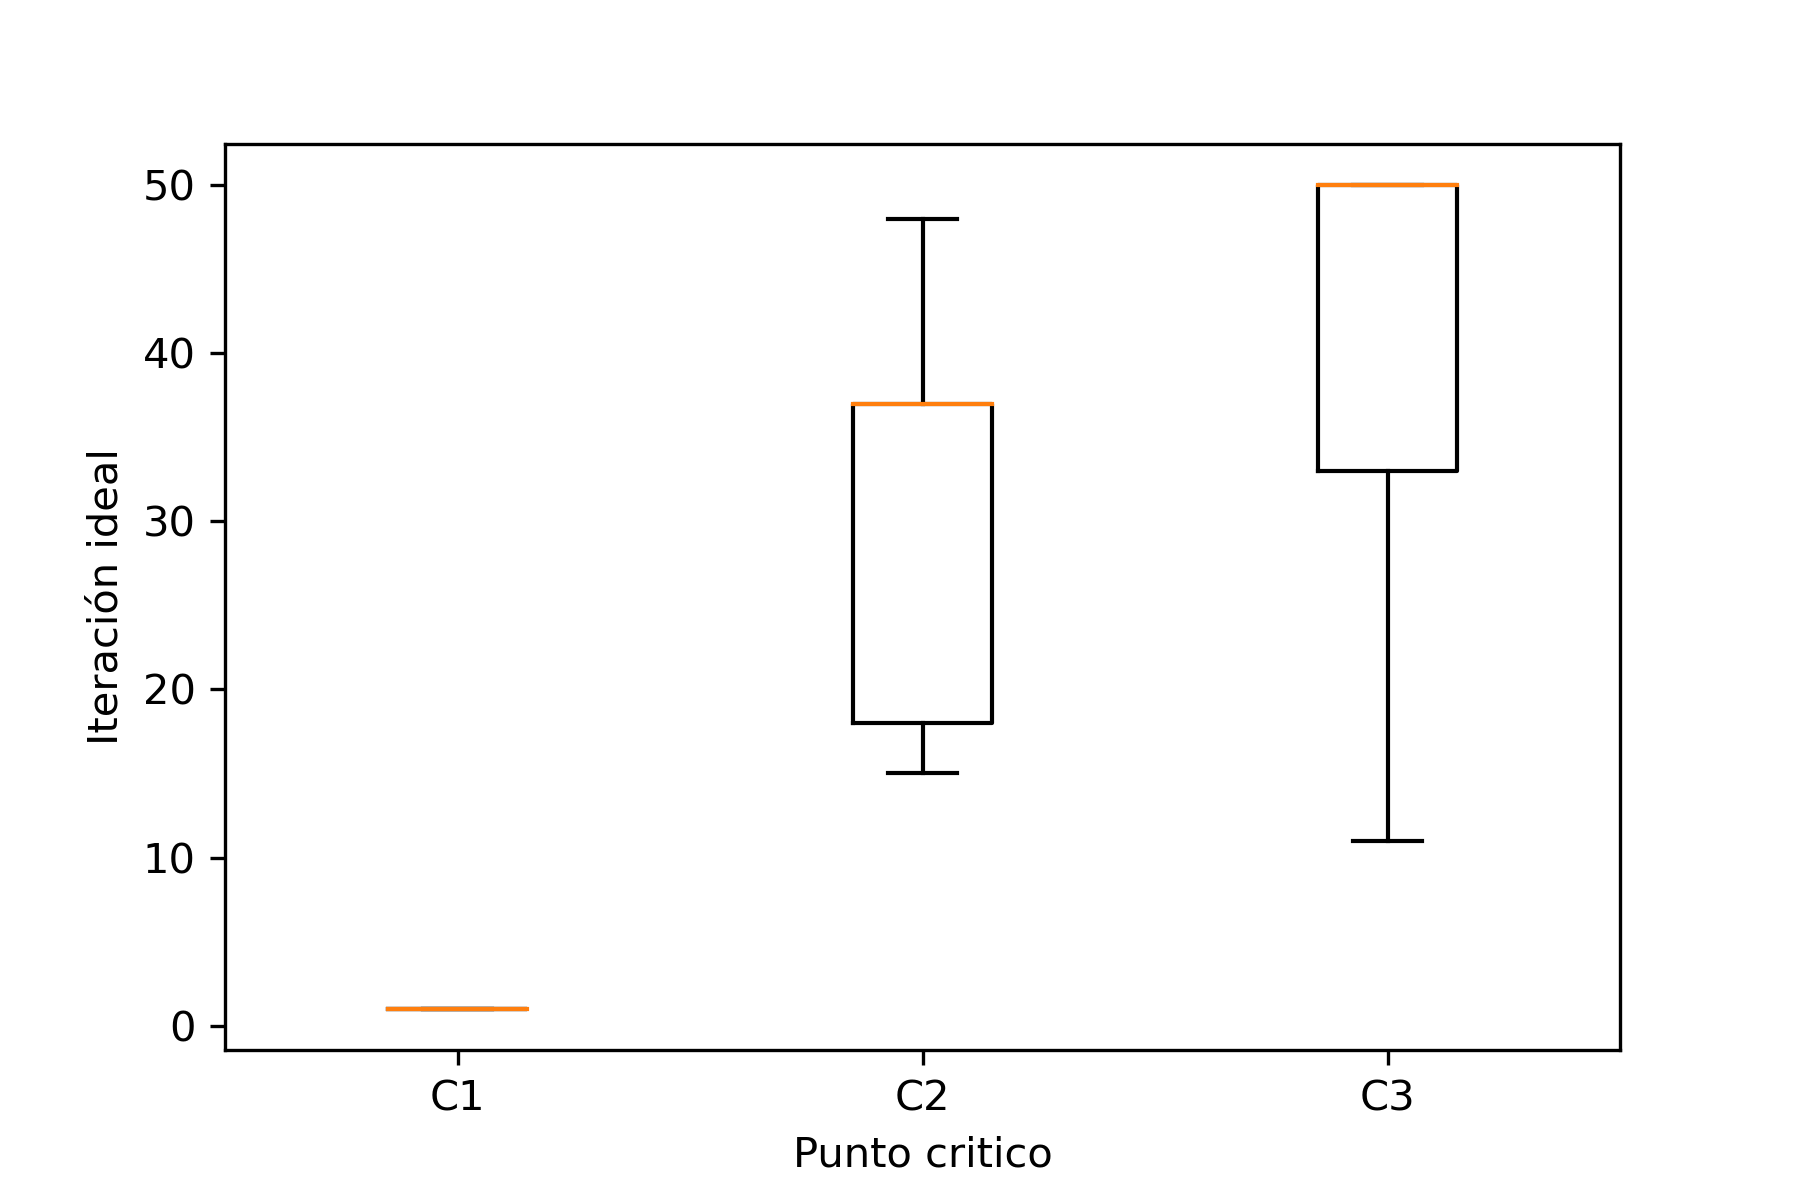
\includegraphics[width=80mm]{p8_v2_r1_c2_n2.png}
\caption{\label{fig3} Gráfica caja bigote de iteración ideal con diferentes puntos críticos.}
\end{figure}

\begin{figure}[H]
\centering
\begin{subfigure}[b]{0.40\linewidth}
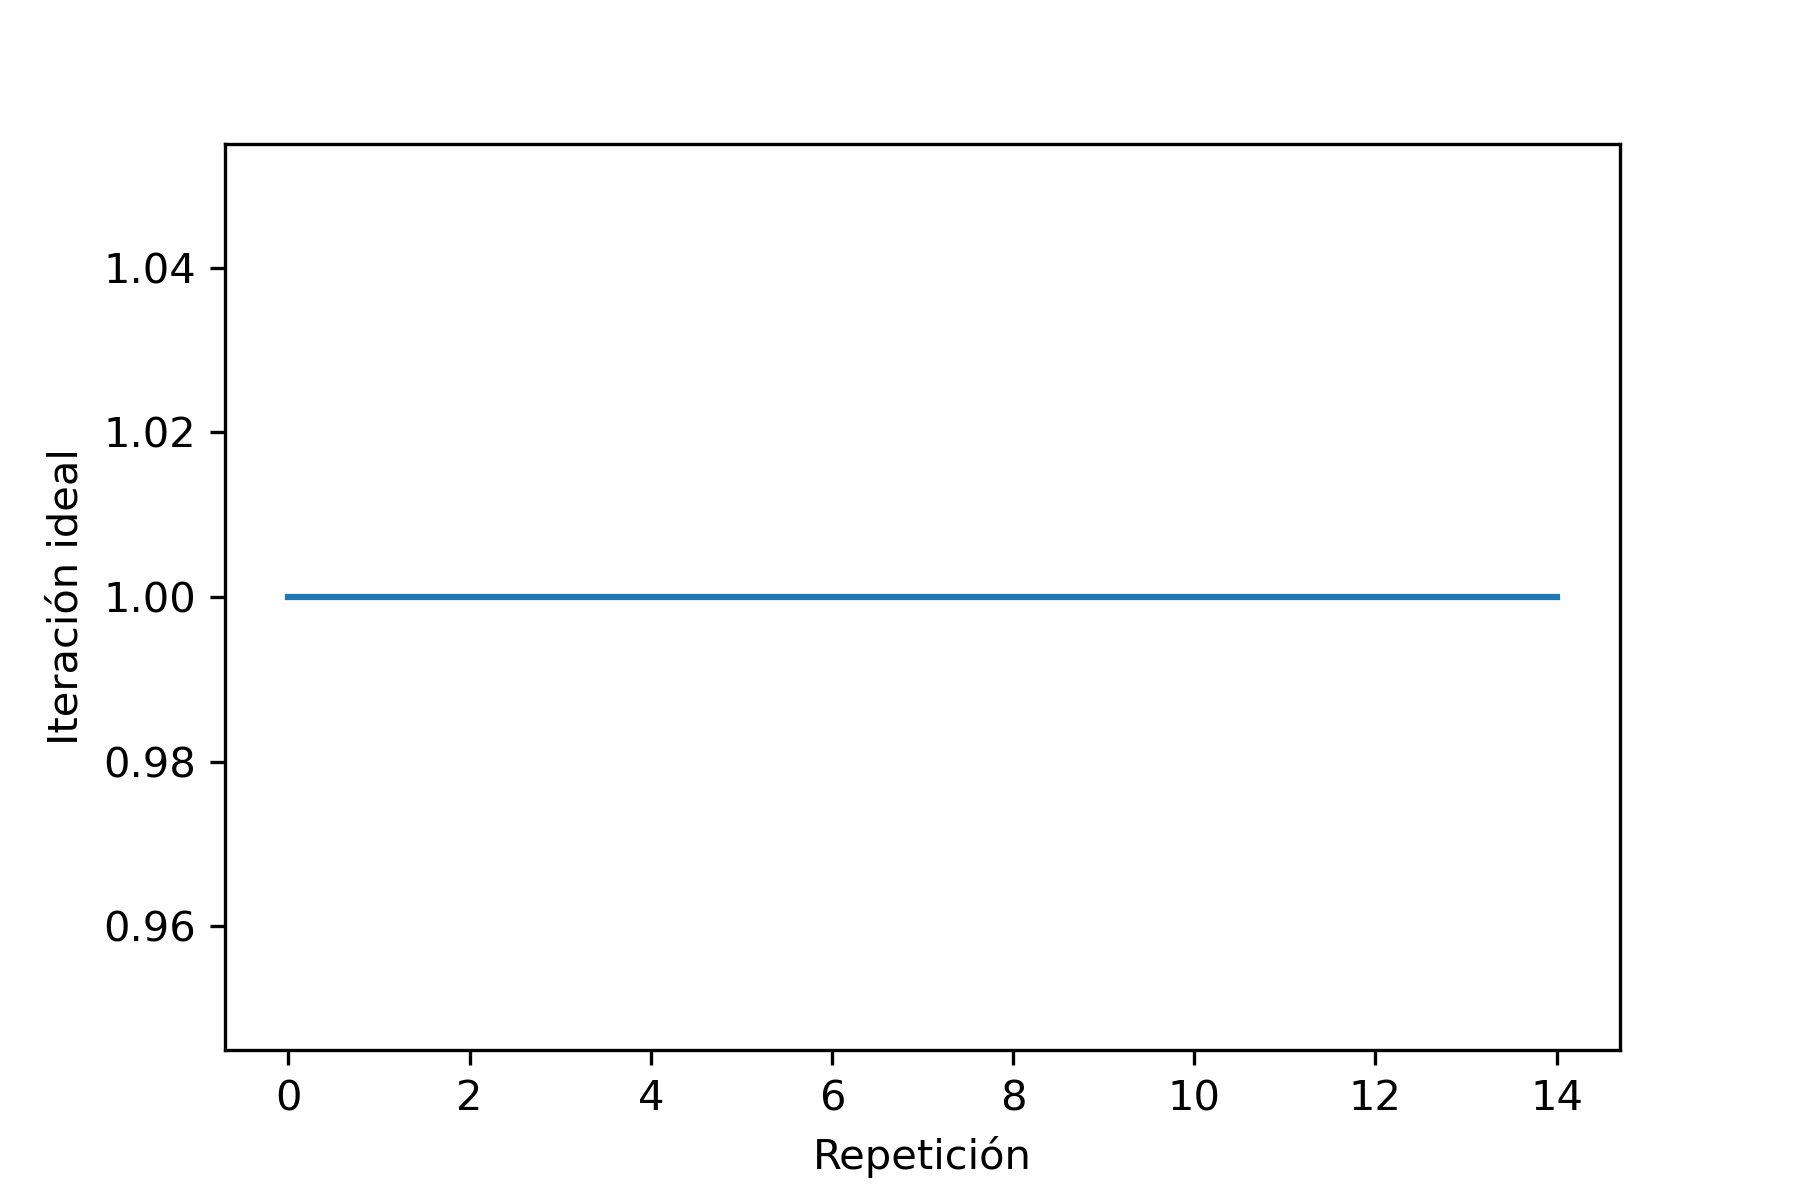
\includegraphics[width=\linewidth]{p8_v2_r1_c0_v3.png}
\caption{128000 partículas en c1.}
\end{subfigure}
\begin{subfigure}[b]{0.40\linewidth}
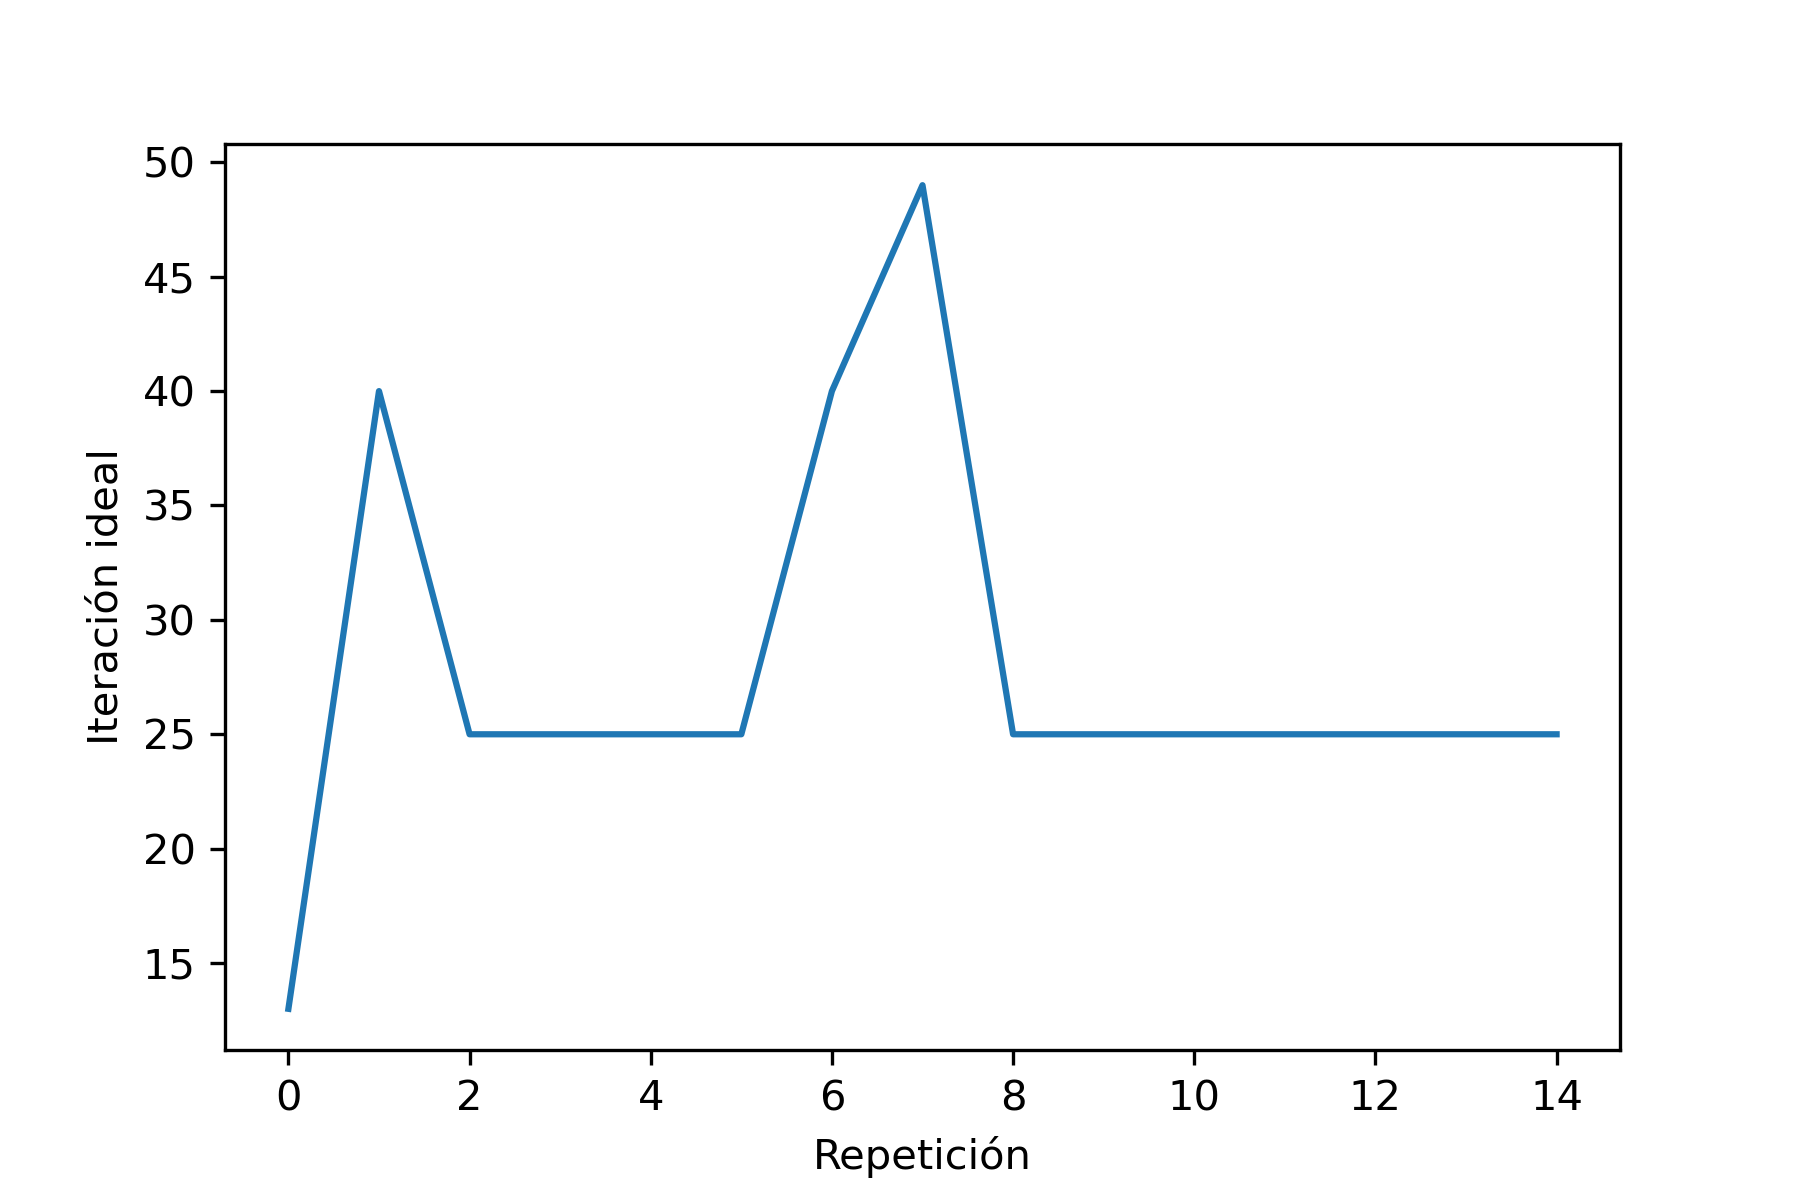
\includegraphics[width=\linewidth]{p8_v2_r1_c1_v3.png}
\caption{128000 partículas en c2.}
\end{subfigure}
\caption{Gráfica de iteración ideal por repetición en diferentes puntos críticos.}
\label{fig:westminster}
\end{figure}

\begin{figure}[H]
\centering
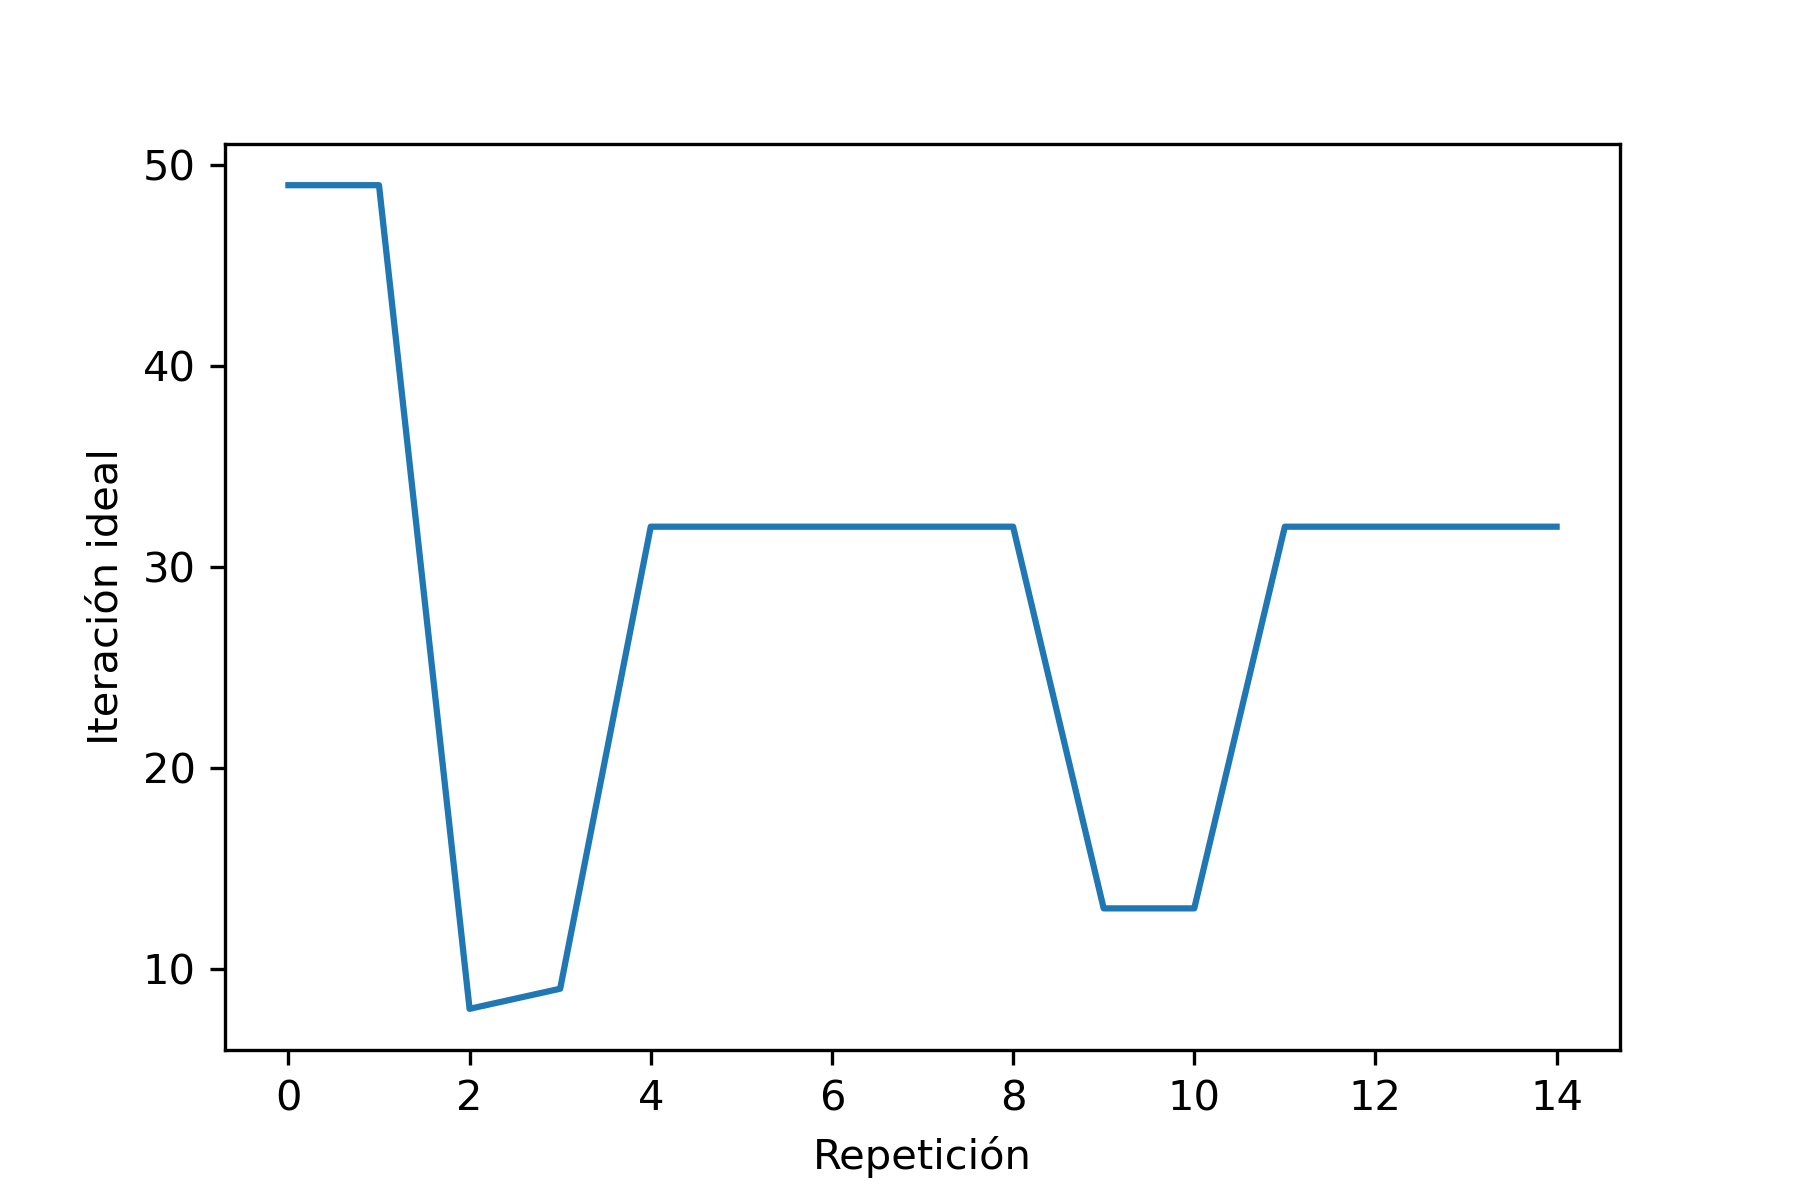
\includegraphics[width=80mm]{p8_v2_r1_c2_v3.png}
\caption{\label{fig3} Gráfica de iteración ideal por repetición en 128000 partículas en c3.}
\end{figure}

\begin{figure}[H]
\centering
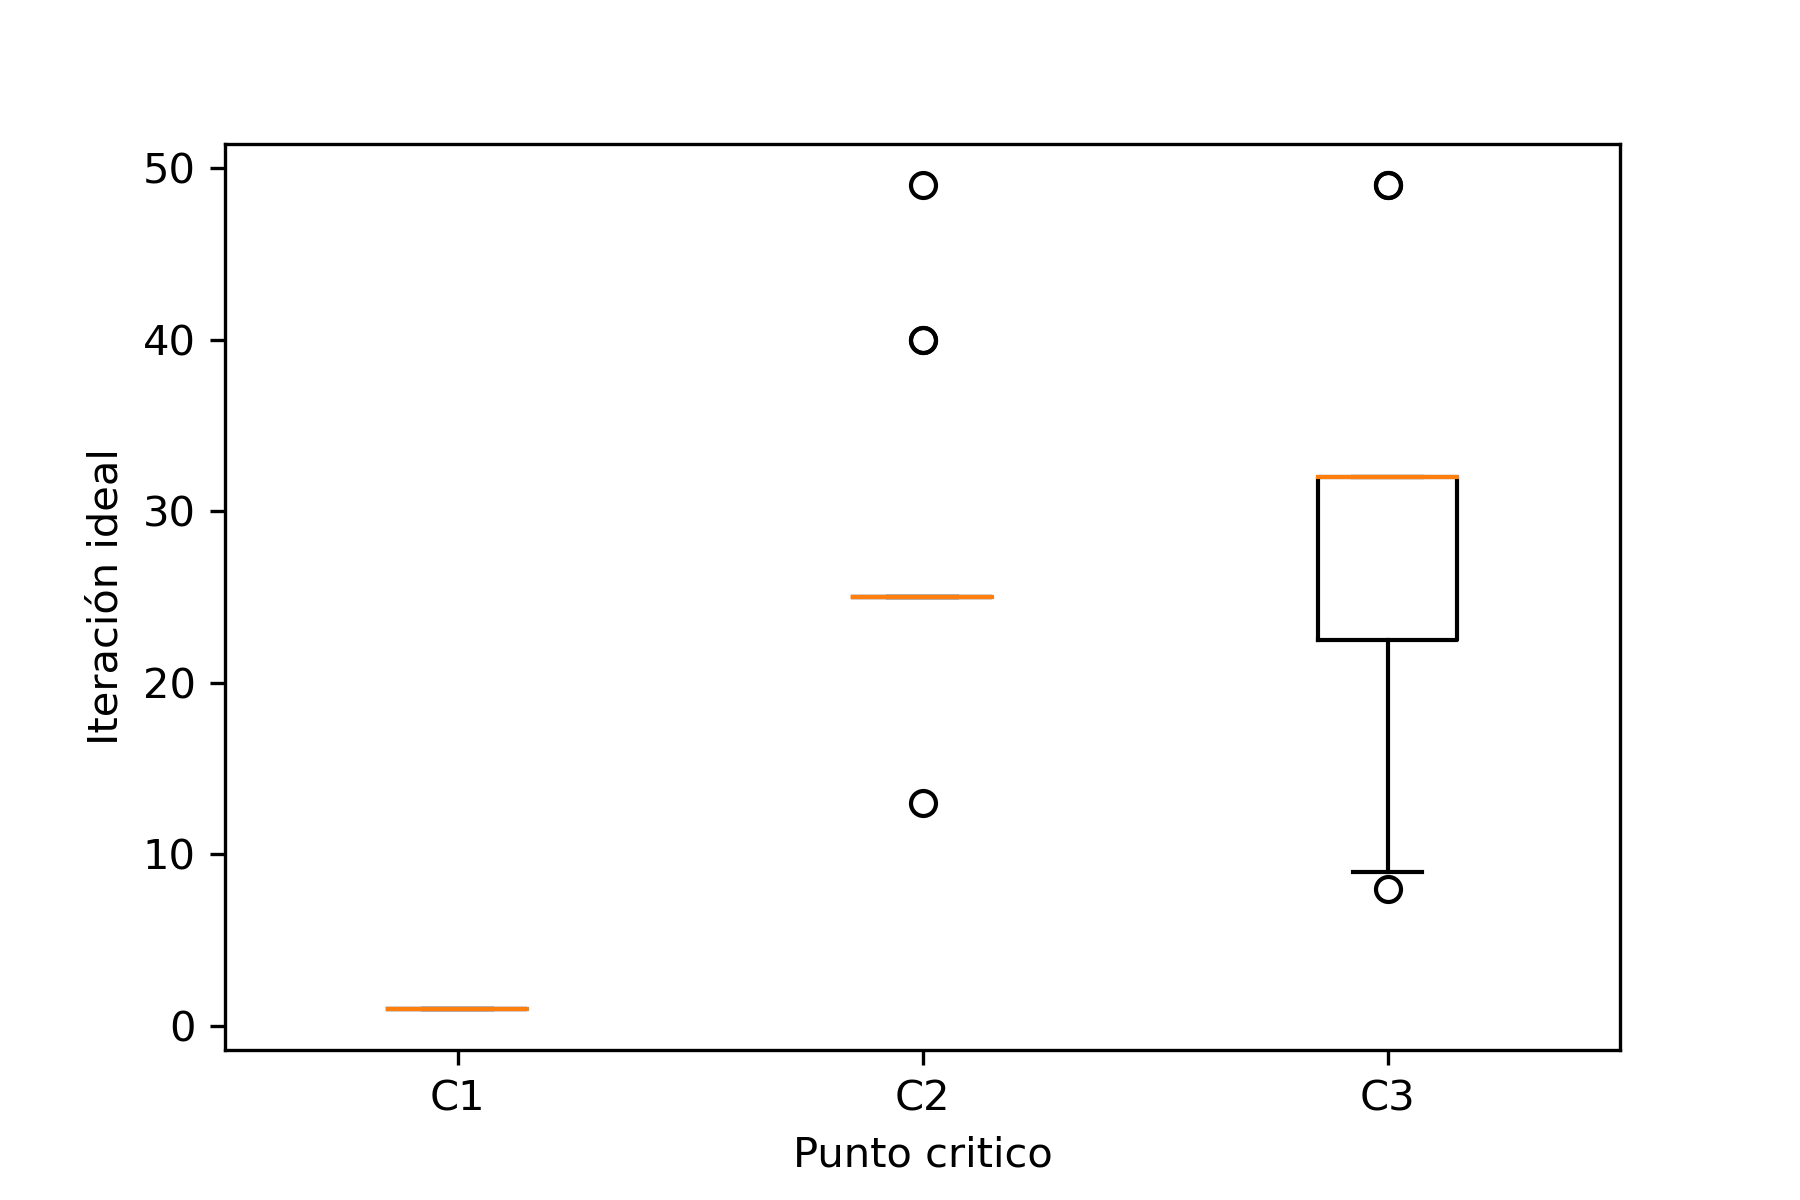
\includegraphics[width=80mm]{p8_v2_r1_c3_n3.png}
\caption{\label{fig3} Gráfica caja bigote de iteración ideal con diferentes puntos críticos.}
\end{figure}

\begin{table}[h!]
\centering
\caption{Prueba estadística Anova.}
 \begin{tabular}{||r r r||} 
 \hline
 Partículas & F & P  \\ [0.5ex] 
 \hline\hline
 16000 & 26.7 & 3.2 \\
 \hline
 32000 & 39.3 & 2.3\\ 
 \hline
 64000 & 66.41 & 9.8  \\
 \hline
 128000 & 47.34 & 1.7 \\
 \hline
\end{tabular}
\label{table:1}
\end{table}

\newpage
\printbibliography
\end{document}
